\documentclass[techmemo]{ecmwfrep}%
\usepackage{graphicx}
\usepackage{caption}
\usepackage{hyperref}
\usepackage{array}
\usepackage{natbib}
\usepackage{subscript}
\usepackage{amsmath}

%%%%%%%%%%%%%%%%%%%%%%%%%%%%%%%%%%%%%%%%%%%%%%%%%%%%%%%%%%%%%%%%%%%%%%%%%%%%
\title{Can global rainfall forecasts identify areas at flash flood risk? Proof of concept for Ecuador}
\headertitle{Can global rainfall forecasts identify areas at flash flood risk? Proof of concept for Ecuador} 
\coverauthor{Fatima M. Pillosu, Agathe Bucherie, Carolynne Hultquist, Andrew Kruczkiewicz, Calum Baugh, Humberto Vergara, Thomas Haiden,  Florian Pappenberger, Elisabeth Stephens, Christel Prudhomme, Hannah L. Cloke\\
University of Reading, ECMWF, etc.
}
\seriesnumber{909}
\date{February 2024}
%%%%%%%%%%%%%%%%%%%%%%%%%%%%%%%%%%%%%%%%%%%%%%%%%%%%%%%%%%%%%

\begin{document}
\maketitle

\begin{abstract}
Globally, flash floods are one of the costliest natural hazards for property damage and loss of life. The low accuracy of flash flood forecasts beyond a few hours limits their use in early warning systems.    The aim of this study is twofold. First, this study aims to assess the performance of probabilistic rainfall forecasts from two different systems - the ECMWF ensemble (ENS) and the ecPoint post-processing system. The forecasts from these two systems are profoundly different: the first system provides forecasts at grid-scale. The second system provides forecasts at point-scale that mirror point observations such as rain gauge. ecPoint rainfall forecasts have been shown to provide better guidance than ENS in the prediction of extreme localized rainfall up to day 10. Hence, ecPoint should enhance ENS performance in the identification of areas at risk of flash floods up to medium-range leads. A one-year objective verification analysis was conducted for flash flood events in Ecuador, whose varied climate and the presence of a comprehensive flood report database made it an attractive site for this type of verification. To carry out such verification analysis, it is imperative to know what the magnitudes of flash-flood-triggering rainfall events are. Since this information was not known by the authors and there were no suitable rainfall observations to estimate such rainfall magnitudes, this study aims to propose a methodology that uses short-term ecPoint-Rainfall forecasts as a proxy for point rainfall observations to define the magnitude of flash-flood-triggering rainfall events to be used in the objective verification analysis. Due to the probabilistic nature of the ecPoint output, this approach allowed the simulation of a very high-density observational network in a de facto data-scarce region. The verification results suggest that ecPoint outperforms ENS in areas where rainfall originates from small-scale convective systems. Where rainfall originates from large-scale convective systems, ecPoint and ENS performances are comparable, except for the better identification by ecPoint of the actual magnitude of the rainfall events. This means that, under certain weather conditions, raw global NWP rainfall forecasts could be used to predict areas at risk of flash floods around the globe up to medium-range leads.  

\end{abstract}

%%%%%%%%%%%%%%%%%%%%%%%%%%%%%%%%%%%%%%%%%%%%%%%%%%%%%%%%%%%%%
\renewcommand{\abstractname}{Plain language summary}
\begin{abstract}
Flash floods cause severe infrastructure damage and loss of life around the globe. Predicting this hazard more than one or two days in advance is very difficult, which makes it extremely difficult to warn people in time. Furthermore, many parts of the world still lack access to predictions for this hazard. This study has two objectives. The first aim addressed in this study relates to the performance analysis of two different global rainfall prediction systems that provide forecasts up to 10 days ahead: the ECMWF ensemble and ecPoint, a post-processing system that provides rainfall predictions for points. The verification analysis was carried out on historical events in Ecuador. Besides having a very diverse climate, Ecuador was chosen because a very detailed flash flood database was developed there to record historical flash flood events in the country. Results show that ecPoint rainfall forecasts accurately identify areas at risk of flash floods where the triggering rainfall event originates from small, localized storms. For more significant, widespread storms, ecPoint and the ECMWF ensemble performed similarly, though ecPoint was better at estimating the magnitude of the most extreme amounts. The second aim addressed in this paper relates to the computation of rainfall thresholds that define flash-flood-triggering rainfall events for forecast verification. This research addressed this problem by considering short-range ecPoint rainfall forecasts as proxies for rainfall observations. Results show that using this approach makes it possible to define rainfall thresholds closer to those calculated using rain gauge measurements (considered the gold standard for this type of analysis), and it would be possible to do so also for ungauged regions. These positive local results give hope that, with further research, ecPoint could be used to predict areas at risk of flash floods over a continuous global domain, with forecast lead times of up to 10 days.

\end{abstract}
%%%%%%%%%%%%%%%%%%%%%%%%%%%%%%%%%%%%%%%%%%%%%%%%%%%%%%%%%%%%%

\section{Introduction}
\label{sec:Introduction}

Flash floods cause significant societal, economic, and environmental impacts \citep{Dordevic2020, Jonkman2008a}. They can occur due to prolonged moderate-to-extreme rainfall or extreme rainfall over a short-term period, leading to a sudden rise of river water levels or the inundation of low-lying areas \citep{Speight2021, Zanchetta2020}. In Latin America, flash flood impacts are exacerbated by rapid, unregulated urbanization of floodplains, human-induced catchment degradation, high poverty levels, lack of preparedness plans, and inadequate infrastructure \citep{Pinos2022}. For example, flash floods in Ecuador are the deadliest form of flooding, and long-term impacts include infrastructure damage, agricultural losses, business and education interruptions, health service disruptions, and waterborne disease outbreaks \citep{Galarza-Villamar2018}. Approximately 60\% of all floods in Ecuador are flash floods \citep{Kruczkiewicz2021a}, and their frequency is expected to increase due to climate change \citep{Hirabayashi2021}. This study aims to enhance preparedness and mitigation strategies against this escalating threat, particularly in regions with limited resources and data, by assessing the effectiveness of global rainfall forecasts in identifying areas at risk of flash floods. It is worth noting that, in this study, the term “identification of areas at risk of flash floods” refers to the prediction of polygons – or areas – that might experience flash flooding due to the expected rainfall. 

Forecast-triggered mitigation strategies, such as early warning systems \citep{Coughlan2022, Sakic2022} and forecast-based financing protocols \citep{Bischiniotis2019, DePerez2016}, have been shown to improve resilience, decrease mortality, and lower recovery costs against riverine floods. Yet, these strategies hinge on accurate, timely predictions. In lower-income countries, accurate forecasts with even longer lead times are required to set cost-effective mitigation strategies \citep{Bazo2019, Kiptum2023}. Over the years, flash flood forecasting systems have been developed at local/regional \citep{Corral2019, Ibarreche2020, RamosFilho2021, Shuvo2021, Speight2018}, national \citep{Javelle2016, Liu2018a}, and continental scale \citep{Gourley2017, Raynaud2015}, with different degrees of model complexity and forecast accuracy. Due to large uncertainties in their forecasting chain, flash floods are more difficult to predict than riverine floods \citep{Speight2021, Zanchetta2020}. Poor historical data on flash flood occurrence and impact \citep{Lowrie2022}, inaccurate predictions of extreme localised rainfall \citep{Zeman2021}, and challenging representation of detailed hydrological processes dependent on topography, soil conditions, and terrain coverage that modulate flash flood occurrence and severity \citep{Xing2019} limit the predictability of flash floods. Thus, forecast-triggered mitigation strategies have been limited for flash floods \citep{DePerez2016}.

Several studies have found that low-complexity, index-based systems using key predictors like rainfall and soil moisture can offer more accurate flash flood predictions than more complex, physically-based models, especially in larger domain systems \citep{Alfieri2015a, Hurford2012, Luong2021, Ma2021, Raynaud2015, Zanchetta2022}. However, the prevailing belief that high-density observational networks \citep{Javelle2010} or km-scale rainfall forecasts \citep{Davolio2017, Song2019} are needed to represent the features of flash-flood-triggering rainfall events has limited the development of a flash flood forecasting system that provides medium-range forecasts over a continuous global domain. Radar-derived rainfall predictions extend only a few hours ahead \citep{Imhoff2022} and the skill of km-scale rainfall forecasts decreases significantly after day 2 lead time \cite{Barrett2019}. Furthermore, their spatial coverage is patchy. Due to the limitations outlined above, the Flash Flood Guidance System with Global Coverage is not developed over a continuous global domain but is built instead on a patchwork of systems over multiple locations \citep{Georgakakos2021}. Consequently, many areas of the world still remain without access to flash flood guidance, highlighting the need for alternative approaches to address the challenge of providing medium-range flash flood predictions over a continuous global domain.

Global Numerical Weather Prediction (NWP) models, such as the ECMWF's Integrated Forecasting System, are increasingly seen as a viable solution to this challenge. These models provide daily global rainfall predictions up to medium-range leads but have historically struggled to accurately predict extreme localized rainfall events due to their coarse resolution and parametrization schemes \citep{Emerton2016, Wen2021}. Owing to recent improvements in global NWP forecast accuracy \citep{Haiden2023, Lavers2021}, the interest in using them to provide flash flood guidance in data-scarce regions and extend predictions' lead times has recently increased \citep{Bucherie2022b}. In addition, the development of state-of-the-art post-processing techniques can improve the quality of the raw forecasts and make them more suitable for flash flood prediction \citep{Vannitsem2021}. For example, the ecPoint statistical post-processing technique transforms global grid-based forecasts into probabilistic point-scale predictions and improves the reliability and discrimination ability of rainfall forecasts up to day 10, especially for extremes \citep{Hewson2021}.

Since there remains a significant gap in leveraging global rainfall NWP forecasts for flash flood forecasting, this study aims to bridge this gap by evaluating and comparing the performance of ENS and ecPoint rainfall forecasts in identifying areas at risk of flash floods. Ecuador, with its extensive flash flood database and high susceptibility to flash flooding, serves as an ideal test bed for this research \citep{Kruczkiewicz2021a}. Two research questions are posed in this study. Can short-range ecPoint rainfall forecasts be used as proxies for in-situ rainfall observations in data-scarce regions to establish rainfall thresholds for an objective flash flood verification analysis? How well do ENS and ecPoint rainfall forecasts identify areas at risk of flash floods? The innovation of this research is threefold. First, it provides a complete objective verification analysis of forecasting systems, including estimates of forecast reliability and discrimination ability, to provide a nuanced assessment of the systems' performance. Second, rainfall forecasts are assessed against rainfall observations, and their suitability for flash flood prediction is simply assumed \citep{Gascon2023, Hewson2021}. The objective verification in this study is conducted using historical flash flood reports in recognition of the non-linear relationship between flash floods and triggering rainfall events. Third, it proposes using short-range ecPoint rainfall forecasts as proxies for in-situ observations in data-scarce regions to calculate the flash-flood-triggering rainfall thresholds to be used in objective verification. 

This paper is organized as follows. Section \ref{sec:Background} provides background information on Ecuador's geography and rainfall/flood climatology. Sections \ref{sec:Data} and \ref{sec:Methods} describe the data and methods used in the verification analysis. Section \ref{sec:Results} presents the results of the objective verification analysis, while section \ref{sec:Case_Study} presents results from a case-study-based subjective verification analysis. Section \ref{sec:Discussion} discusses the verification results, and section \ref{sec:Conclusions} draws concluding remarks for the study.


%%%%%%%%%%%%%%%%%%%%%%%%%%%%%%%%%%%%%%%%%%%%%%%%%%%%%%%%%%%%%

\section{Background: geography, rainfall climatology and flooding in Ecuador}
\label{sec:Background}

\begin{figure}
\centering
\includegraphics[width=0.9\textwidth]{Figures/01_BACKGROUND_Ecuador_Orography_RegionsENS_PopulationDensity.png}
\caption{Panel (a) displays Ecuador's topography, outlines its political regions in white, and indicates the location of the country's three main geographical regions: the coast ("La Costa"), the Andean highlands ("La Sierra"), and the Amazon forest ("El Oriente"). The insert highlights Ecuador's location (in red) in South America. Panel (b) shows Ecuador's domain within the ENS and ecPoint grid, with grid boxes indicated with black dots. The regions are colour-coded in yellow for “La Costa”, brown for “La Sierra”, and green for “El Oriente”. Panel (c) shows the population density from the 2020 census (people/km2) in each political region.}
\label{fig:Background}
\end{figure}

Located in north-western South America, Ecuador includes continental Ecuador and the Galápagos Islands in the Pacific Ocean, 1000 km from the mainland (insert in Figure \ref{fig:Background}\hyperref[fig:Background]{a}). The Andes run north to south through Ecuador (Figure \ref{fig:Background}\hyperref[fig:Background]{a}) and split it into three main regions \citep{Vuille2000}: “La Costa”, which comprises the Andes’ western slopes and the coastal plains along the Pacific Ocean; “El Oriente”, which covers a plateau containing 2\% of the Amazon basin and the eastern slopes; and “La Sierra”, which contains the inter-Andean region between the western and eastern slopes of the Andes. This study considers only the continental landmass, hereafter referred to as “Ecuador”. The domain of interest, including the borders with Colombia, Peru, and the Pacific Ocean, contains a total of 1090 grid boxes. This general domain is then split into the three main regions mentioned above using Ecuador’s topography in the ENS grid (Figure \ref{fig:Background}\hyperref[fig:Background]{b}). Grid boxes below 600 m above sea level and to the west and the east of the longitude 78.2 °W belong to “La Costa” (i.e., 321 grid boxes) and “El Oriente” (299 grid boxes). Grid boxes above 600 m were assigned to “La Sierra” region (470 grid boxes).

The rainy season in “La Costa” spans from December to May \citep{Ilbay2021}. Broad-scale atmospheric and oceanic phenomena modulate the intensity and spatial variability of rainfall. The extreme phases of El Niño Southern Oscillation, known as El Niño (i.e., above-average sea surface temperature in the Pacific Ocean) and La Niña (i.e., below-average), enhanced and decreased the average rainfall during the rainy season, respectively \citep{Recalde-Coronel2014, Tobar2018}. In addition, certain phases of the Madden-Julian Oscillation, 1 and 8 (i.e., when a convection centre is over the Western Hemisphere and Africa) and 4 and 5 (i.e., when a convection centre is over the Maritime continent), are associated with an enhancement and decrease in precipitation, respectively \citep{Recalde-Coronel2020}. “La Sierra” has two main rainy seasons (i.e., February-May and October-November). Precipitation spatial patterns in the inter-Andean valleys are more complex than in “La Costa” because rainfall is typically generated by smaller-scale convective systems \citep{Vuille2000}. Additionally, as air masses lose much of their humidity on both flanks of the Andes, precipitation amounts in “la Sierra” are relatively lower than those in the other two regions, varying between 800 and 1500 mm/year \citep{Buytaert2006, Vuille2000}. Several studies \citep{Bendix2006, Buytaert2006, Junquas2022} have shown that in the Andean region, most of the rainfall occurs during the daytime, particularly in the afternoon hours, between 2 pm and 7 pm local time (LT). It rains throughout the year in “El Oriente”, with the wettest (driest) months being April-July (September-October). Rainfall climatology in “El Oriente” is primarily influenced by strong convective activity across the Amazon Forest and water vapor variations from the sea surface temperature of the tropical Atlantic Ocean \citep{Vuille2000}.

Floods cause considerable material loss and deaths in “La Costa” and “La Sierra” because they are heavily populated and contain Ecuador’s two most important industrial areas, Guayaquil in Guayas and Quito in Pichincha 
(Figure \ref{fig:Background}\hyperref[fig:Background]{c}). Prolonged rainfall events in “La Costa” can generate extensive, severe surface runoff far from rivers and cause rivers to flood vast plain areas \citep{Galarza-Villamar2018}. Intense shorter-lived rainfall events (i.e., less than one day) can also cause severe, sudden surface runoff \citep{Galarza-Villamar2018}. Rivers in “La Sierra” are susceptible to extreme localised rainfall events and, consequently, are prone to flash flooding \citep{Laraque2009, Pinos2020}. The river flows in “El Oriente” show a much stronger response to seasonal rainfall than a single rainfall event because of the size and length of Amazonian rivers, floodplain storage, and shallow riverbeds \citep{Trigg2009}.

%%%%%%%%%%%%%%%%%%%%%%%%%%%%%%%%%%%%%%%%%%%%%%%%%%%%%%%%%%%%%

\section{Data}
\label{sec:Data}

This section introduces and provides statistical summaries for the datasets used in this verification analysis. This summary will be useful to interpret the verification results.  

\subsection{Flash flood reports}
\label{sec:Data_ReportsFF}

\begin{figure}
\centering
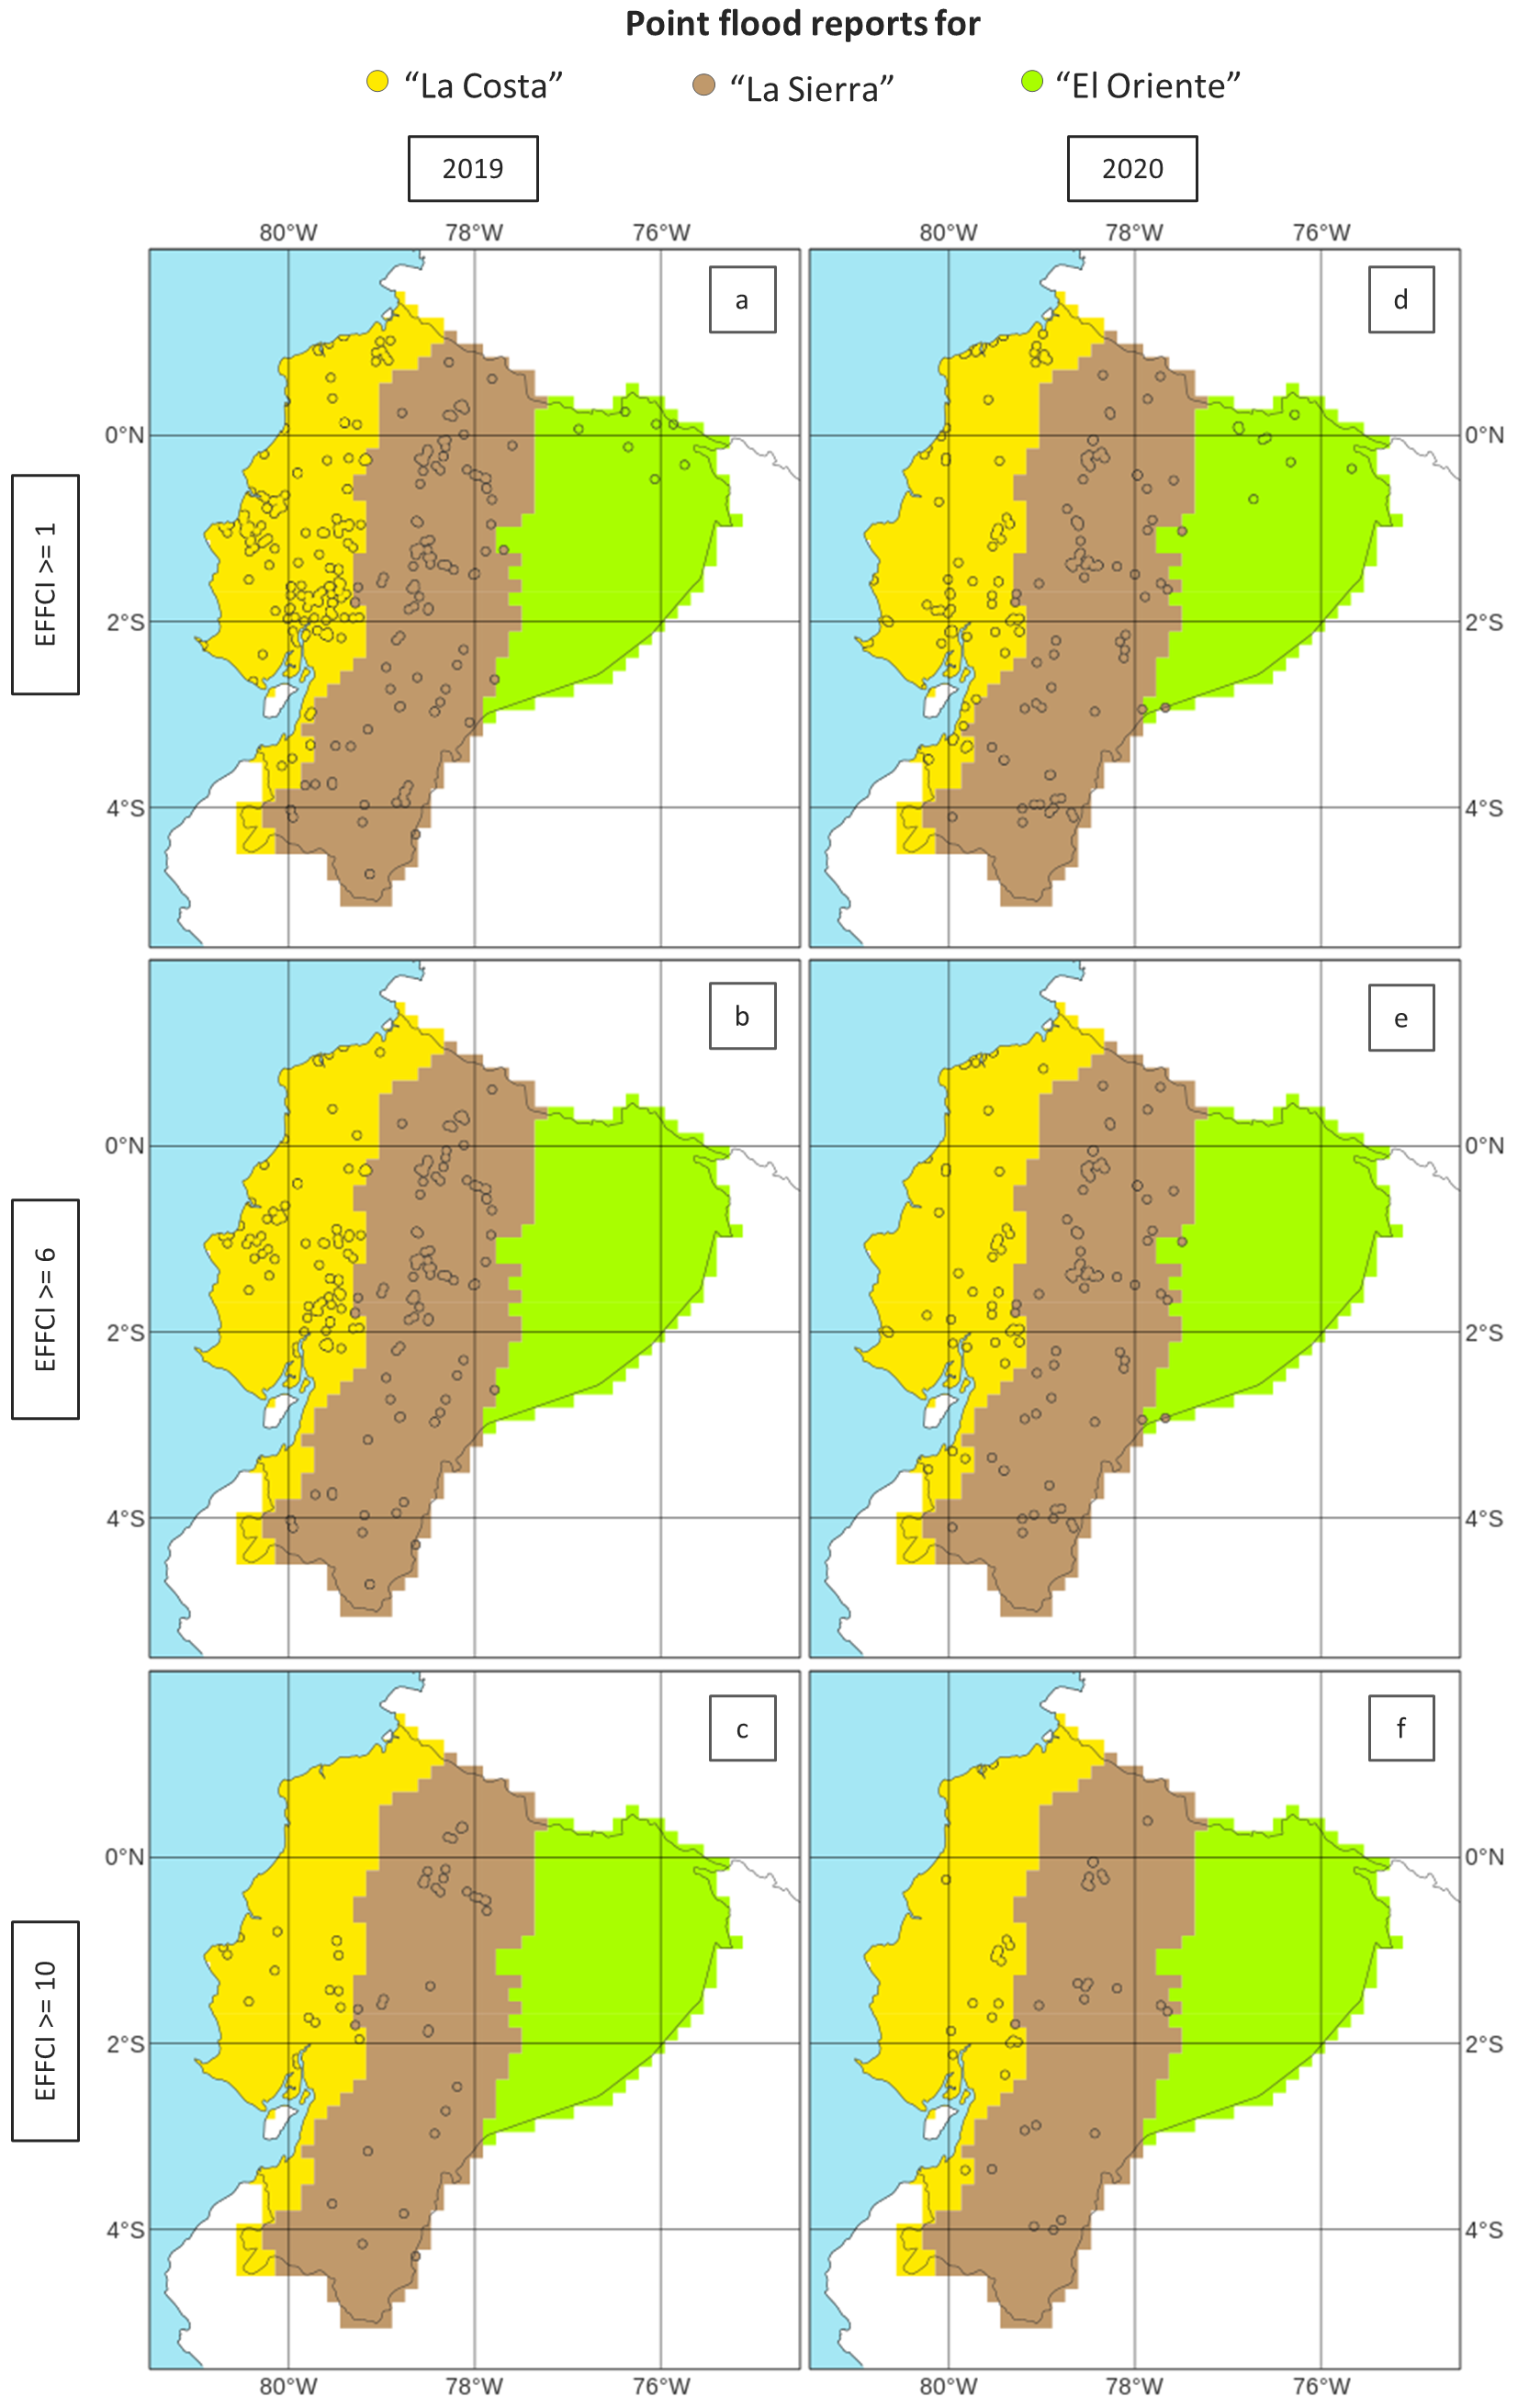
\includegraphics[width=0.85\textwidth]{Figures/02_DATA_PointFR_2019_2020.png}
\caption{Panels (a), (b), and (c) show the spatial distribution of point flood reports in 2019 with EFFCIs, respectively, $\geq$1, 6, and 10. Panels (d), (e), and (f) are the same but for flood reports in 2020.}
\label{fig:PointFR_Maps}
\end{figure}

\begin{figure}
\centering
\captionof{table}{The first column indicates the years considered in this analysis. The second column shows the total number of flood reports in the database in each year. The third column shows the number of excluded reports from the study because they did not contain any reporting location (in lat/lon coordinates) and/or reporting time (with date and time). The fourth column shows the number of remaining flood reports. The remaining columns show the distribution of flood reports per region (C: Costa, S: Sierra, O: Oriente) and EFFCI threshold.}
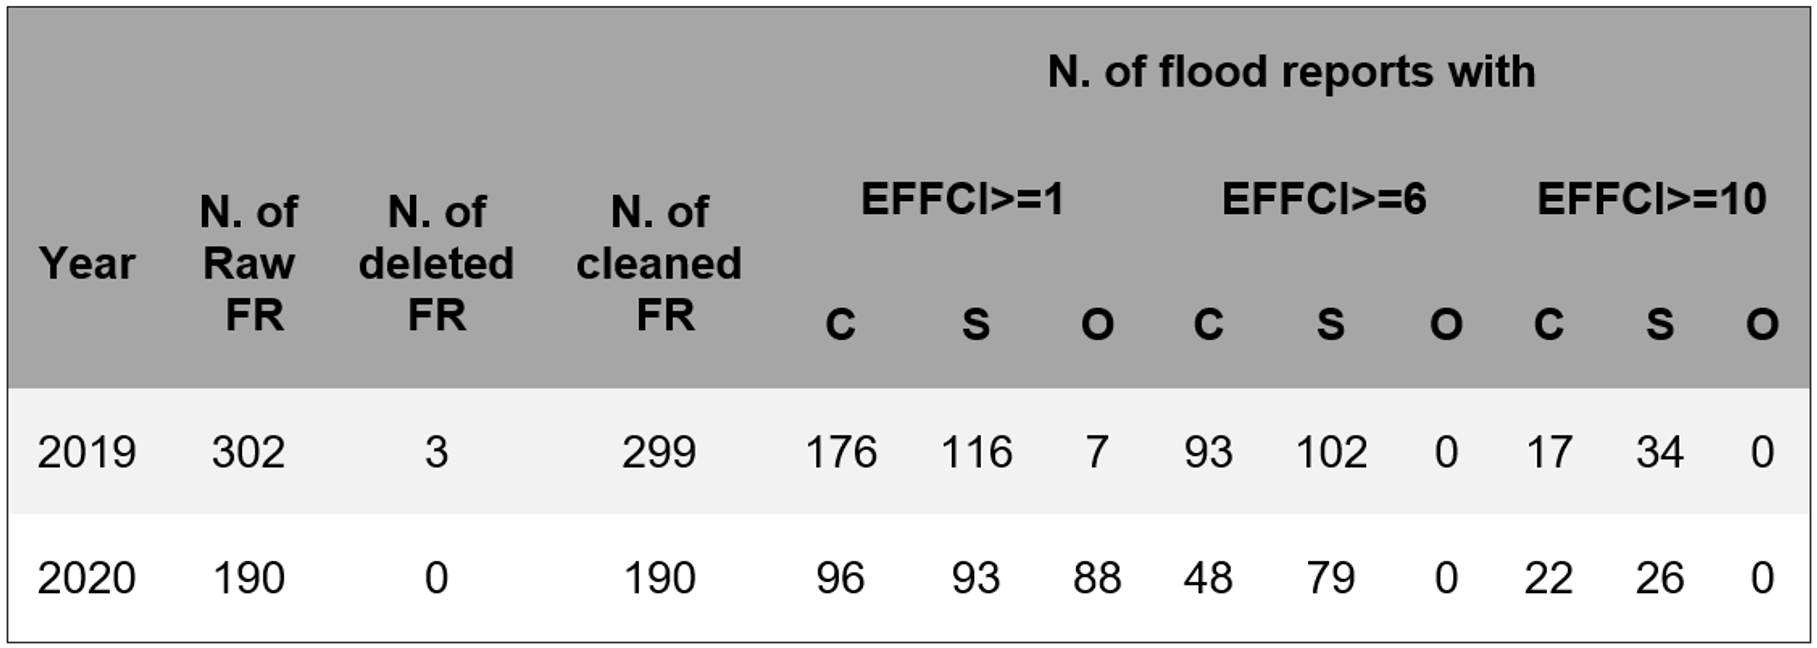
\includegraphics[width=0.6\textwidth]{Tables/01_CountFR_EFFCI.png}
\label{table:CountFR_EFFCI}
\end{figure}

\begin{figure}
\centering
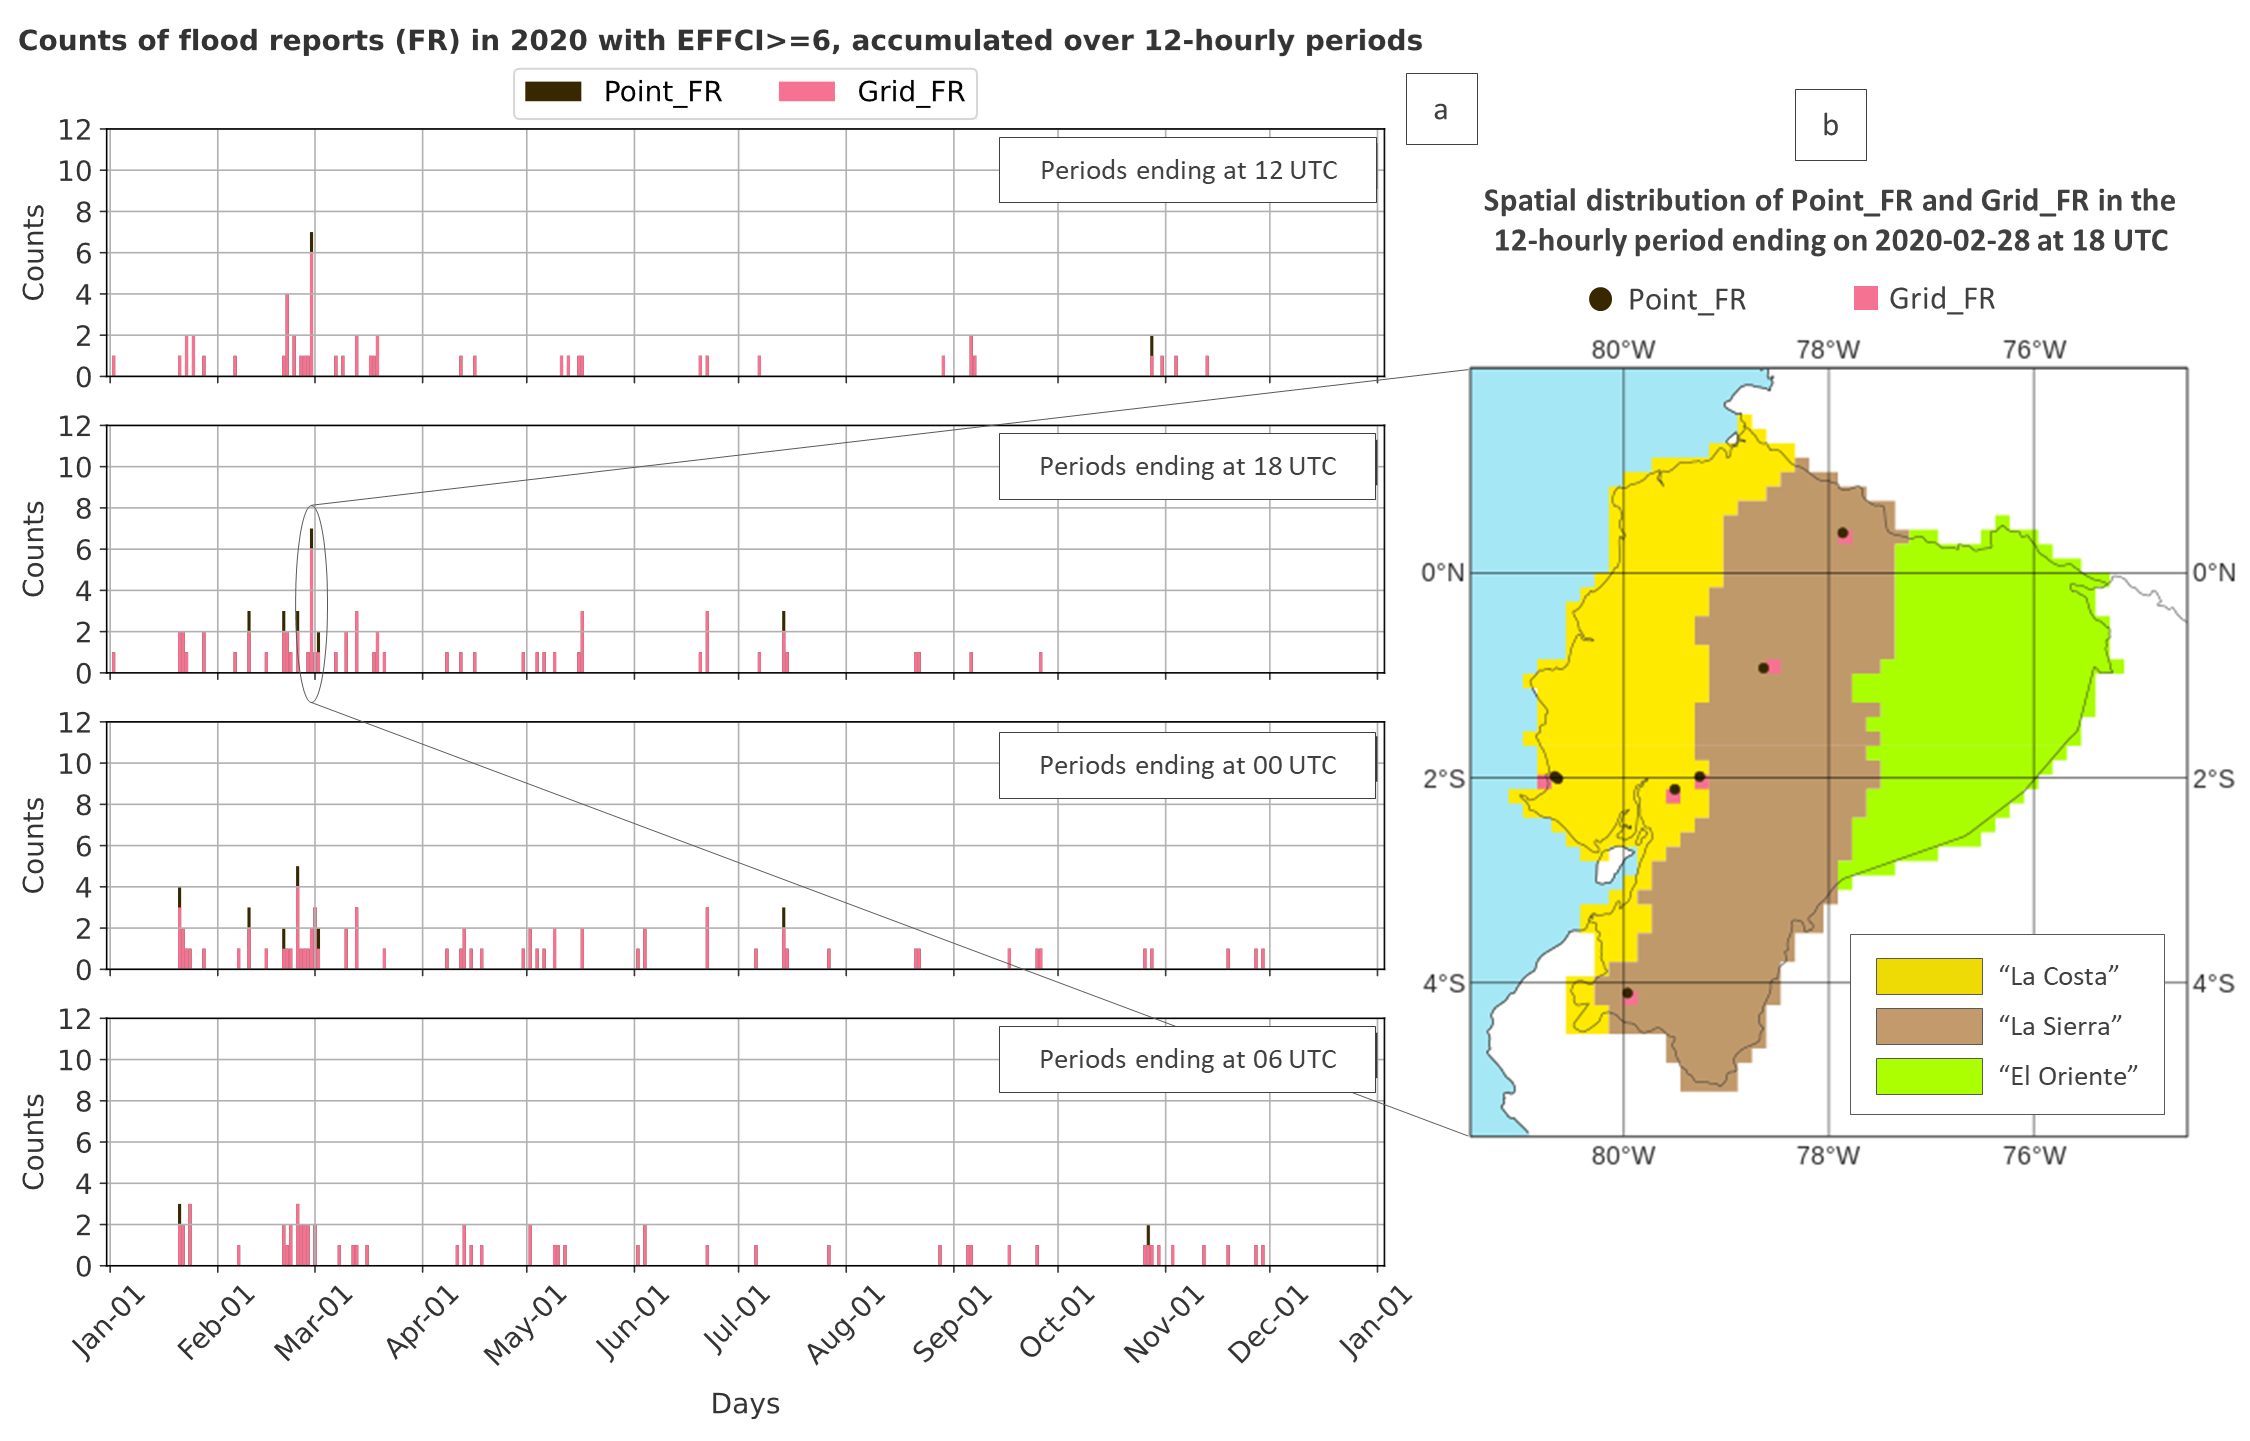
\includegraphics[width=0.95\textwidth]{Figures/03_DATA_Distribution_PointFR_GridFR.png}
\caption{Panel (a) displays the timeseries of the counts of 2020’s flood reports with EFFCI$\geq$6, over four overlapping 12-hourly accumulation periods, ending at 12 (first row), 18 (second row), 00 (third row), and 06 UTC (fourth row). Figure \ref{fig:PointFR_Maps}\hyperref[fig:PointFR_Maps]{e} shows their collective spatial distribution. The overlapped black and pink bars represent point and grid flood reports, respectively. Where the black bars are visible, more than one point flood report was assigned to the grid box. Panel (b) shows the spatial distribution of the point and grid flood reports for the accumulation period that contains the largest number of flood reports, namely the one ending at 18 UTC on 2020-02-28.}
\label{fig:Distr_PointFF}
\end{figure}

Disaggregation by flood type and specific documentation about historical flash flood events and their impacts are rare in many regions of the world, primarily due to a lack of commonly accepted flash flood definitions \citep{Bucherie2022a, Kruczkiewicz2021b}. \cite{Kruczkiewicz2021a} developed a method to assign an “Enhanced Flash Flood Confidence Index (EFFCI)” for flood events in historical flood datasets, based on text mining of disaster reports and a flash flood susceptibility index extracted from the geophysical properties of the location of the events. The EFFCI is an estimate of the likelihood of a flood event being a flash flood, ranging from 1 (not very likely) to 10 (extremely likely). The flash flood database in Ecuador was mainly compiled from two datasets, DesInventar \citep{UNDRR2021} and the Ecuadorian Secretariat for Disaster Management (SNGRE), and it contains 4967 flood events from 2007 to 2020. In addition to the EFFCI index, most entries in the flash flood database contain information about the location (with latitude and longitude coordinates) and the day and time (in local time) of flood occurrence. As a result of applying this method to Ecuador, a historical dataset of flood occurrences and impacts is available, with specific information on the likelihood of events being flash floods \citep{Bucherie2021}. Although this dataset is the best attempt to address historical flash floods in Ecuador, it is essential to note that it is based on disaster reporting processes carried out on the ground and not systematically collected over time. Consequently, it can present gaps, inconsistent descriptions of flood processes over time, and uncertainty in geolocation. 

This study considered flood reports from 2019 to define the climatology of rainfall events associated with flash floods. Events from 2020 were used to perform an objective verification analysis. Three EFFCI thresholds were considered to evaluate the impact of uncertainty around a flood report as a flash flood event: EFFCI$\geq$1 (all flood reports), EFFCI$\geq$6 (flood reports that are likely to be flash floods), and EFFCI$\geq$10 (flood reports that are highly likely to be flash floods). Table \ref{table:CountFR_EFFCI} shows the total number of flood reports in 2019 and 2020, as well as their distribution between the three considered regions and EFFCIs. Figure \ref{fig:PointFR_Maps} shows the spatial distribution of such flood reports, while Figure \ref{fig:Distr_PointFF} shows the time distribution of flash flood reports with EFFCI$\geq$6.

\subsection{Rainfall observations}
\label{sec:Data_RainOBS}

\begin{figure}
\centering
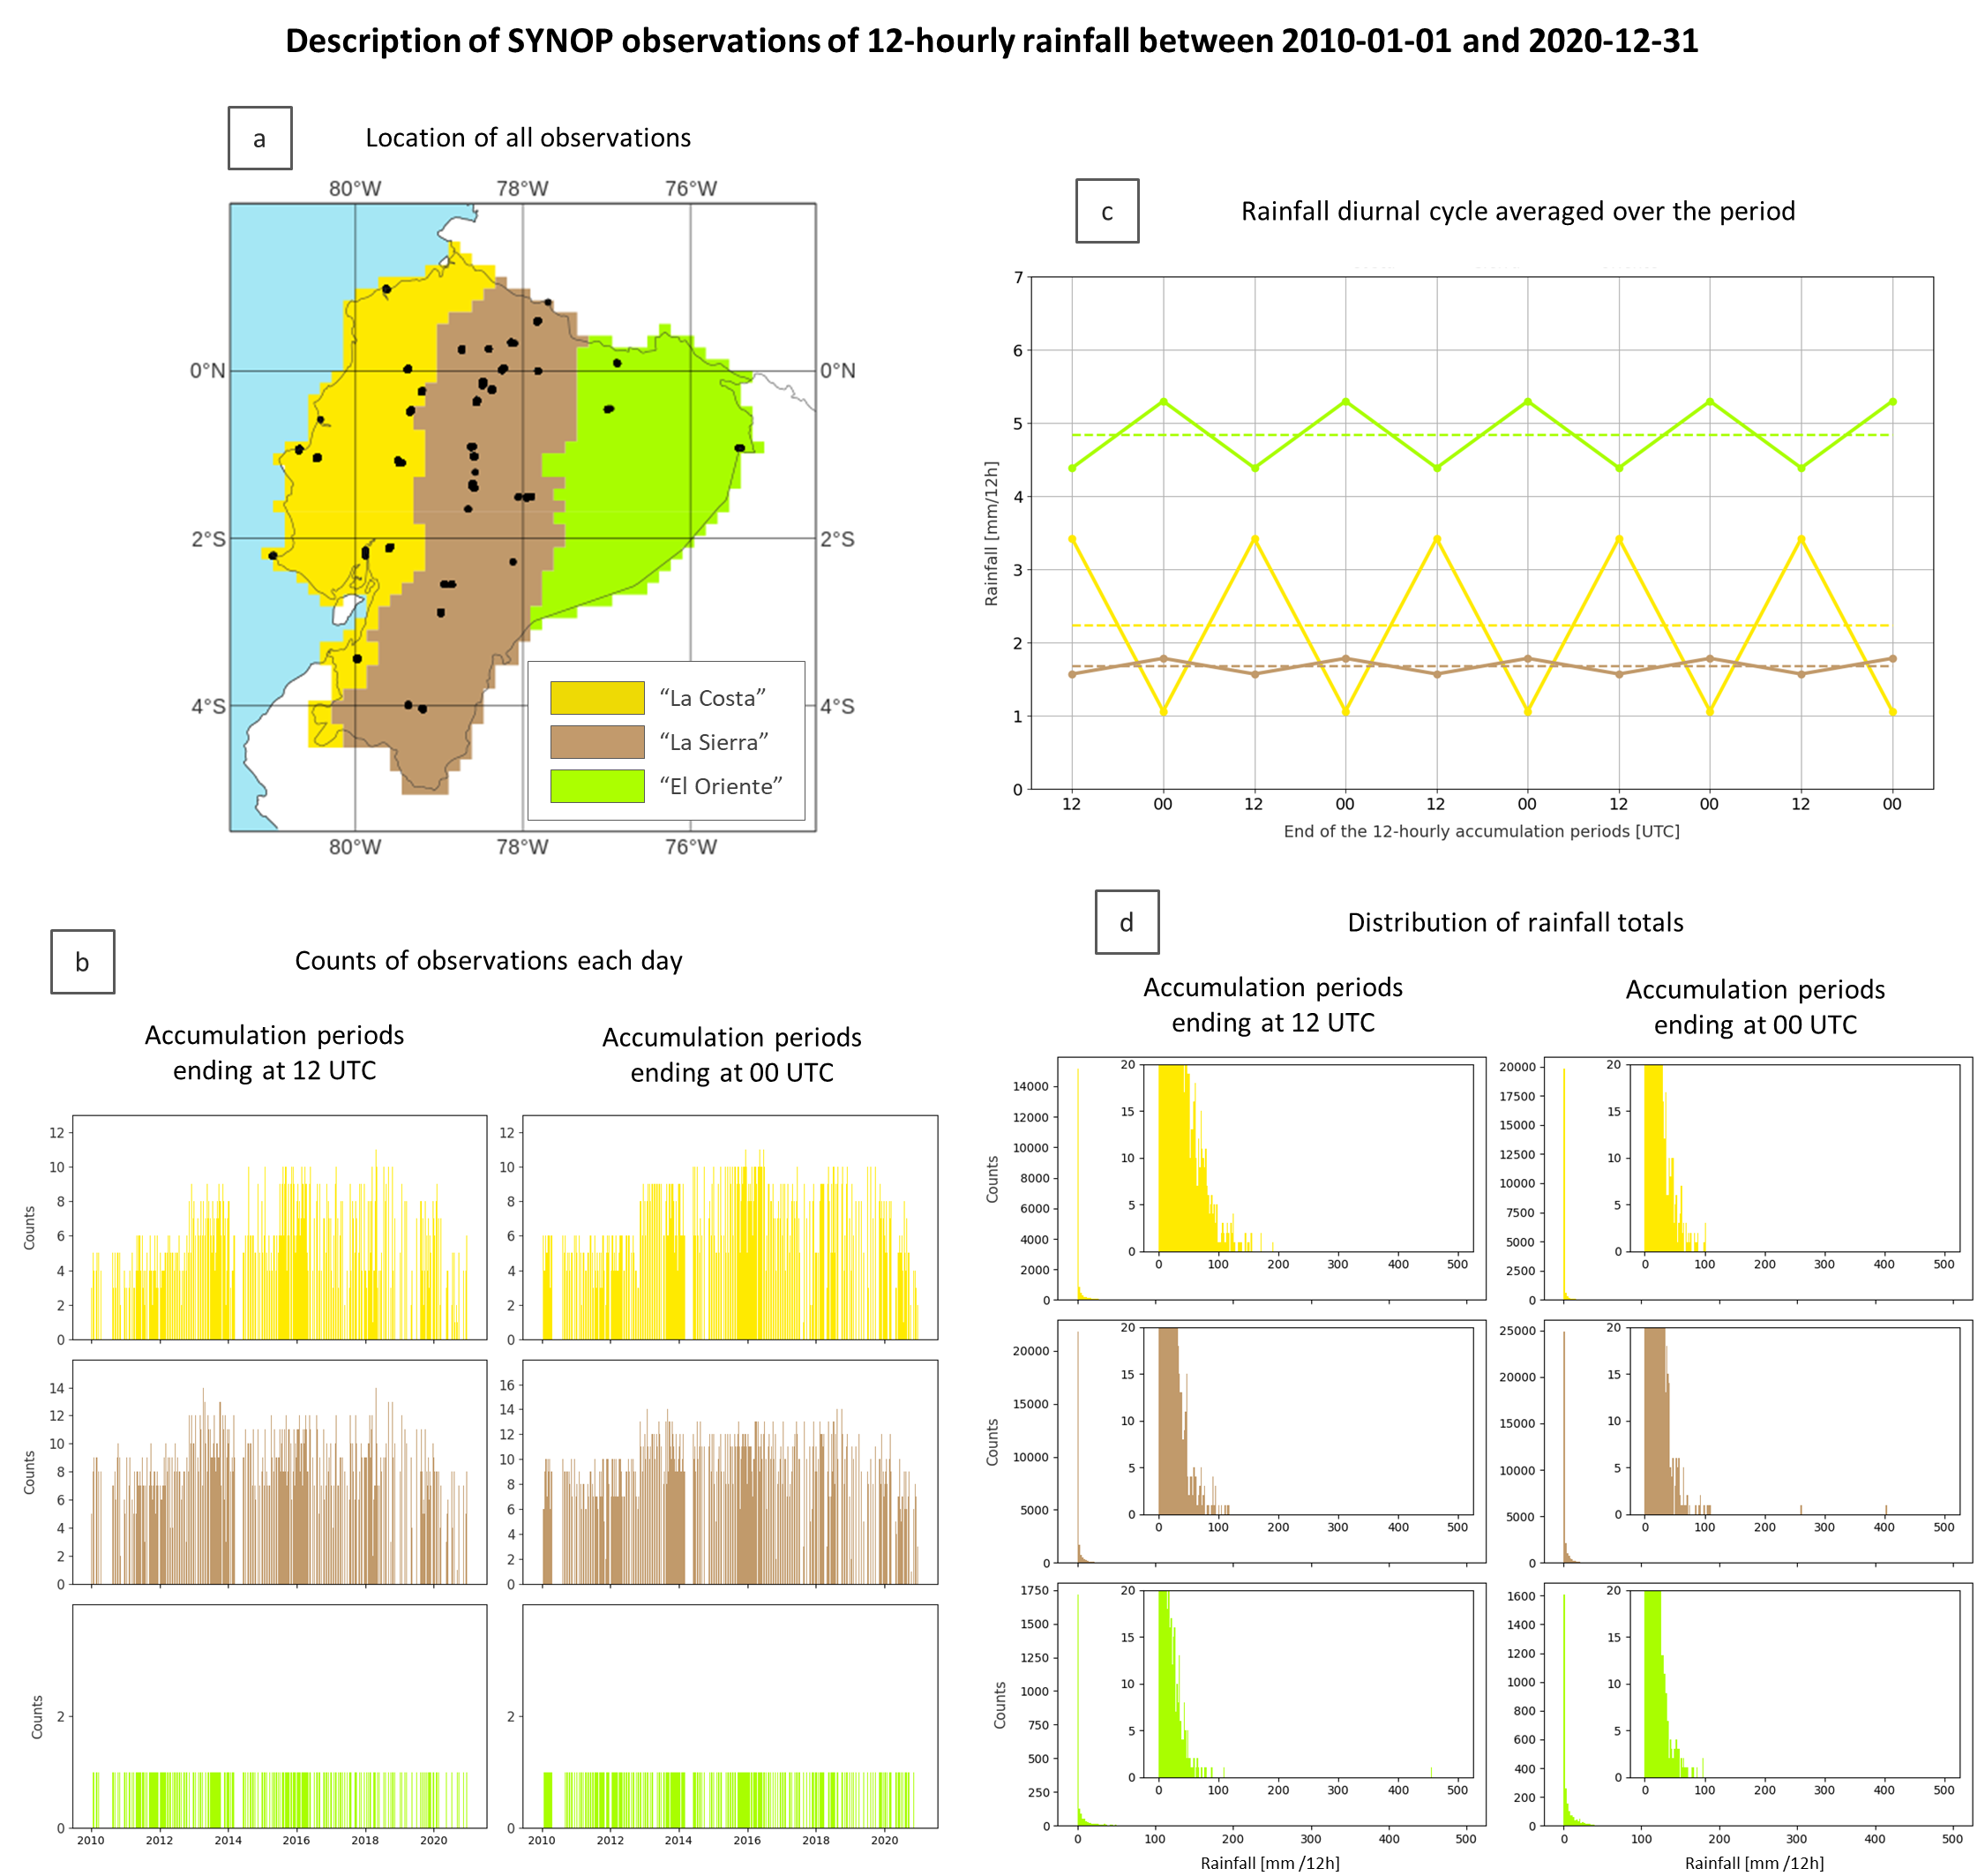
\includegraphics[width=\textwidth]{Figures/04_DATA_Description_SYNOP_rainfall.png}
\caption{Description of 12-hourly SYNOP rainfall observations in Ecuador from 2010-01-01 to 2020-12-31. Only accumulation periods ending at 12 and 00 UTC were available. Each plot is colour-coded according to the region they refer to: yellow for “La Costa”, brown for “La Sierra”, and green for “El Oriente”. Panel (a) displays a map plot with the location of all SYNOP observations (some might have moved locations over time). Panel (b) shows the daily counts of observations available for the accumulation period ending at 12 UTC (first column) and at 00 UTC (second column). Panel (c) shows the average rainfall for all considered years, for the accumulation period ending at 12 and at 00 UTC (the two values are repeated five times in the plot), and the corresponding trend lines. In panel (d), the distributions of 12-hourly rainfall totals are shown for the accumulation period ending at 12 UTC (first column) and at 00 UTC (second column). Each distribution includes zoomed-in inserts to remove the focus over the very small rainfall totals.}
\label{fig:Descriptio_SYNOP}
\end{figure}

Rainfall observations from the SYNOP network transmitted by the Global Telecommunication System (GTS) were used in this study to represent Ecuador’s rainfall climatology and provide a context for both the estimated rainfall totals associated with flash flood events and the objective verification results. In the ECMWF’s internal database, only 12-hourly rainfall observations with accumulation periods ending at 00 and 12 UTC, between the 1st of January 2010 and the 31st of December 2020, are available for Ecuador. Figure \ref{fig:Descriptio_SYNOP}\hyperref[fig:Descriptio_SYNOP]{a} and Figure \ref{fig:Descriptio_SYNOP}\hyperref[fig:Descriptio_SYNOP]{b} show their spatial and temporal distribution, respectively. Not all days have observations. “El Oriente” has only one observation in a given day, while most of the days in “La Costa” and “La Sierra” have 4 to 8 observations in a given day, with peaks of 10 observations in “La Costa” and 14 in “La Sierra”. Figure \ref{fig:Descriptio_SYNOP}\hyperref[fig:Descriptio_SYNOP]{c} shows the average rainfall over the entire study period for each accumulation period. The sinusoidal pattern in all three regions confirms what was reported in Section \ref{sec:Background} regarding the marked rainfall diurnal cycle in Ecuador. From the available observations, “La Costa” is the region with the most marked rainfall diurnal cycle with peak at night-time (i.e., accumulation period ending at 12 UTC) of $\sim$3.5 mm/12h and troughs at daytime (i.e., accumulation period ending at 00 UTC) of $\sim$1 mm/12h, and an average rainfall overall of $\sim$2.2 mm/12h. “La Sierra” shows instead a very small diurnal cycle with an amplitude of just $\sim$0.1 mm/12h between night-time and daytime rain, and an average of $\sim$1.6 mm/12h. It also appears that the times at which peaks and troughs occur are inverted to those in “La Costa”.  Although the spatial coverage of the rainfall observations in “El Oriente” is very poor, it is possible to observe that the average rainfall in the rain forest is substantially bigger than in the other two regions (i.e., $\sim${}4.8 mm/12h) and that the amplitude of the rainfall’s diurnal cycle is $\sim$1 mm/12h. Figure \ref{fig:Descriptio_SYNOP}\hyperref[fig:Descriptio_SYNOP]{d} shows the distribution of the rainfall totals on a given day for each accumulation period. More than 50\% of the observations were less than 1 mm. “La Costa” is the region that has more frequent observations above 100 mm/12h in the accumulation period ending at 12 UTC, which corresponds to the local night-time. During daytime rain (i.e., accumulation period ending at 00 UTC) in “La Costa”, and in both accumulation periods in “La Sierra” is rare to observe any rainfall $\geq$ 100 mm/12h. However, it is possible to observe two extreme rainfall observations in the  accumulation period ending at 00 UTC in “La Sierra” of up to $\sim$260 and $\sim$400 mm/12h. 

\subsection{Rainfall forecasts: ECMWF ENS and ecPoint}
\label{sec:Data_RainFC}

\begin{figure}
\centering
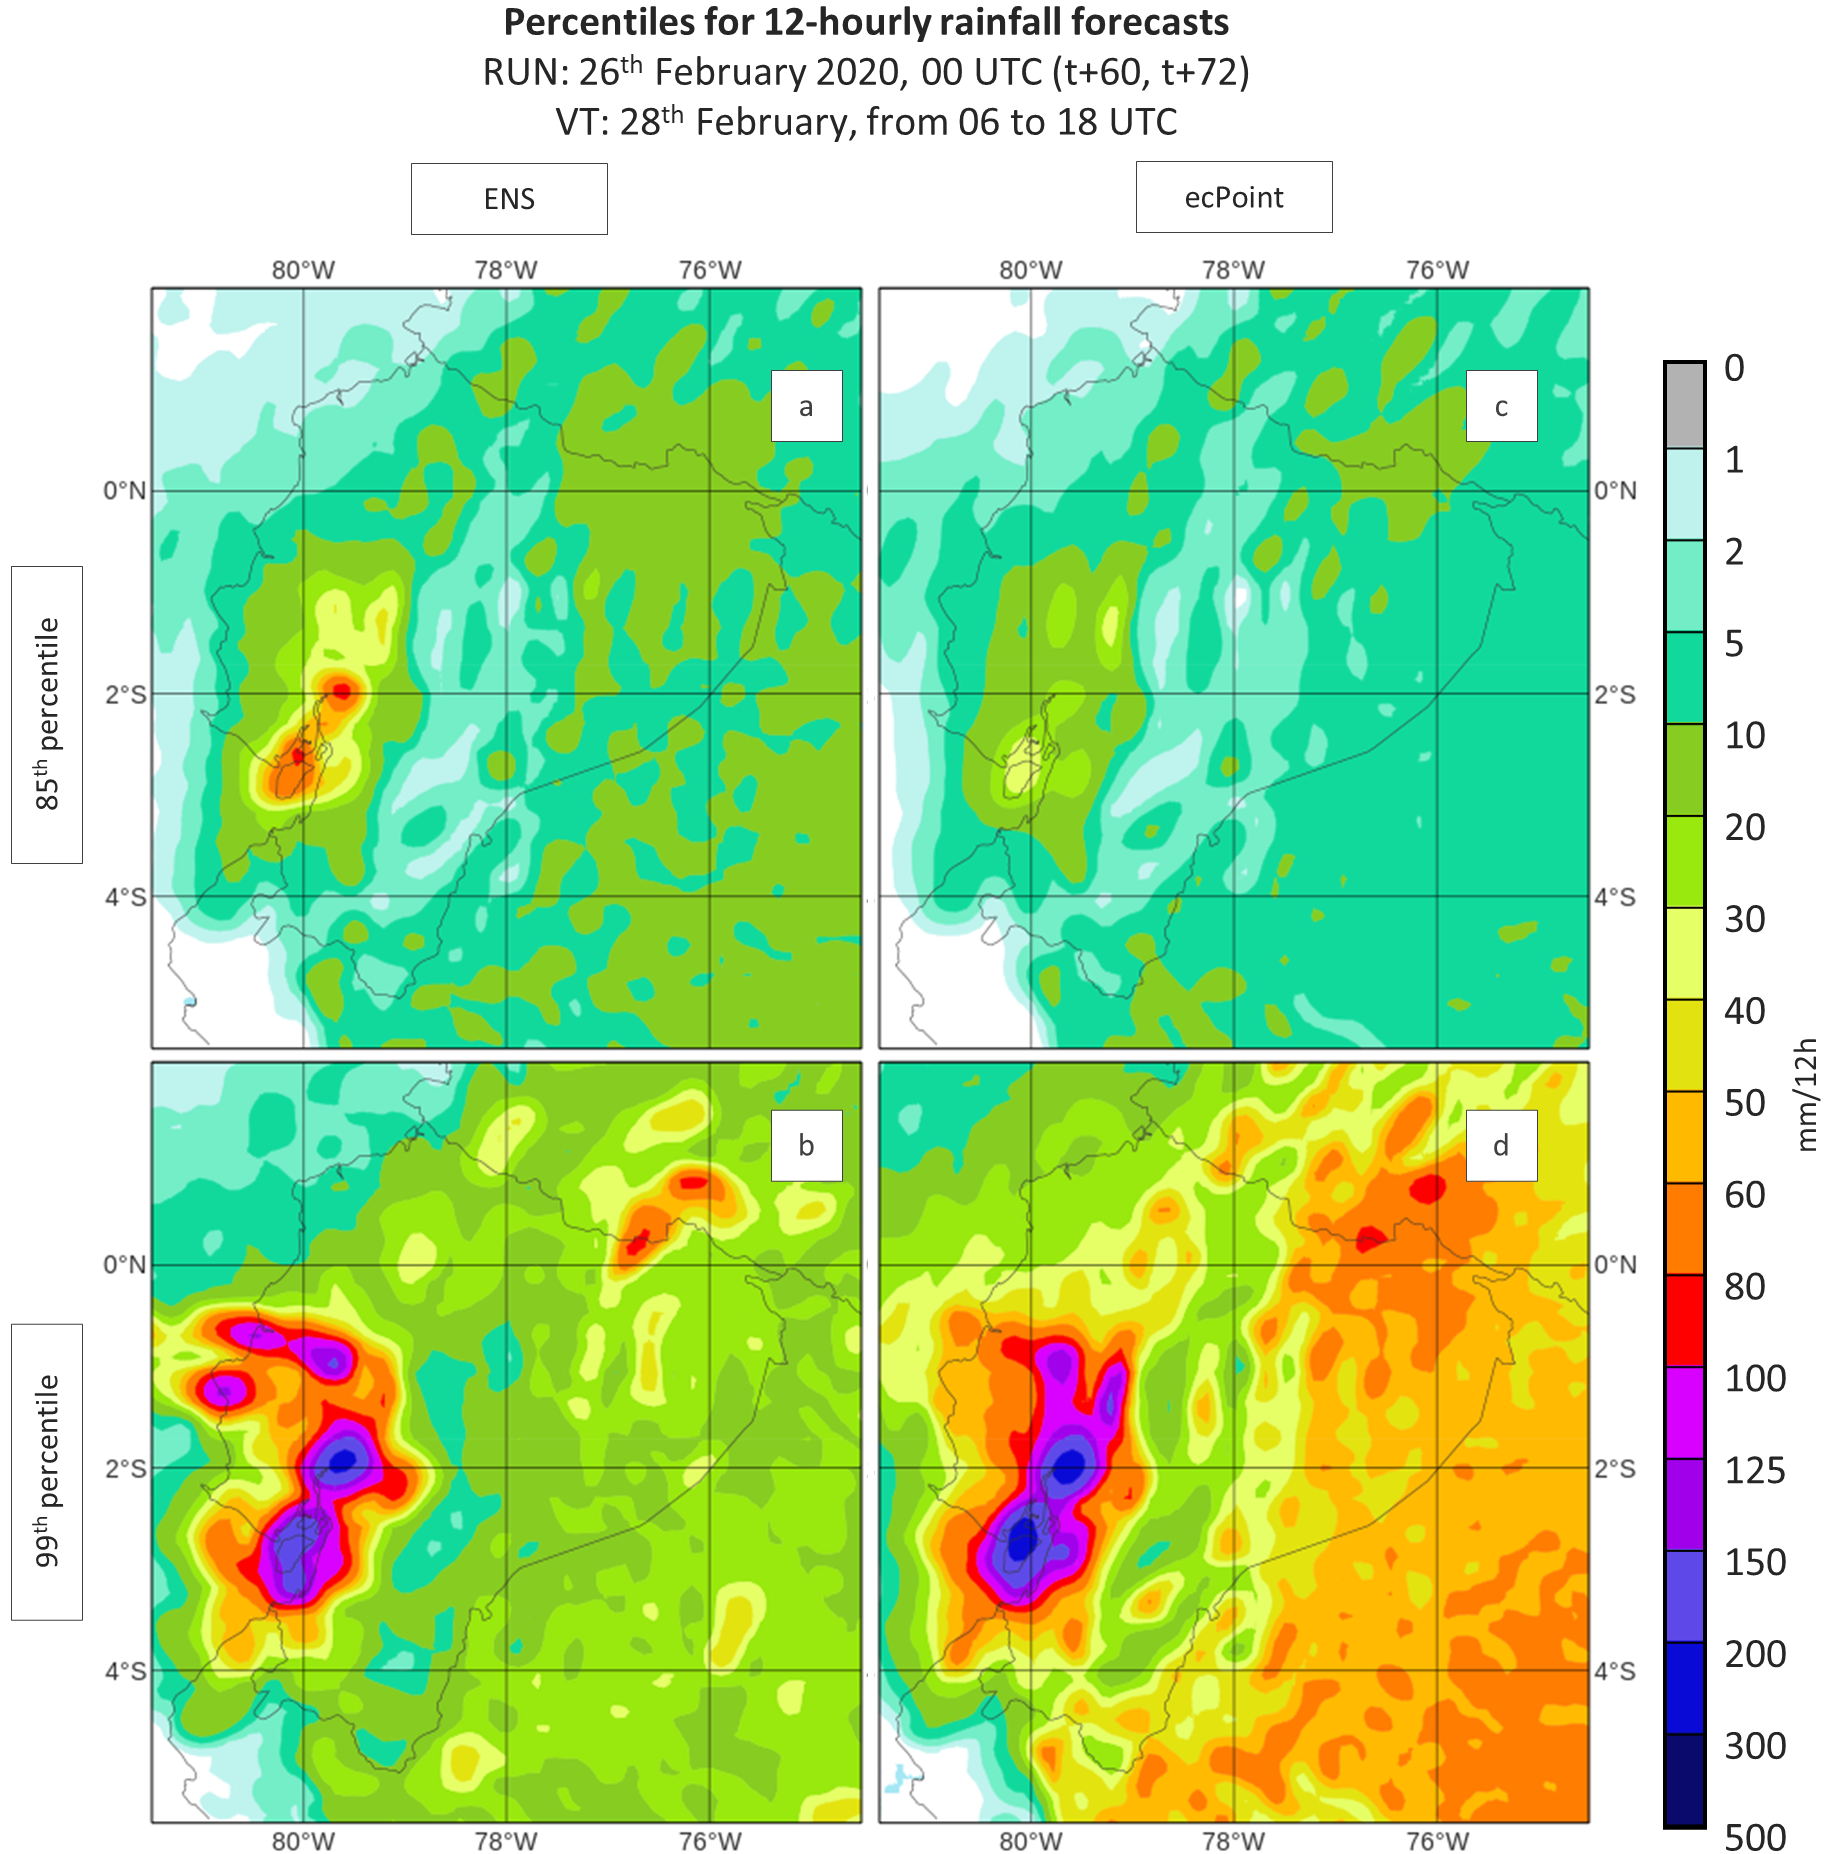
\includegraphics[width=0.7\textwidth]{Figures/05_DATA_Percentiles.png}
\caption{Example of a probabilistic ENS (first column) and ecPoint (second column) medium-range rainfall forecast (in mm/12h). The forecast is from the midnight run (00 UTC) on the 26th of February 2020, for the accumulation period ending at t+72, and valid for the 28th of February 2020 between 06 and 18 UTC (i.e., 00 and 12 LT). Panels (a) and (c) show examples of the 85th percentile for ENS and ecPoint, respectively, while panels (b) and (d) show examples of the 99th percentile.}
\label{fig:Percentiles}
\end{figure}

\begin{figure}
\centering
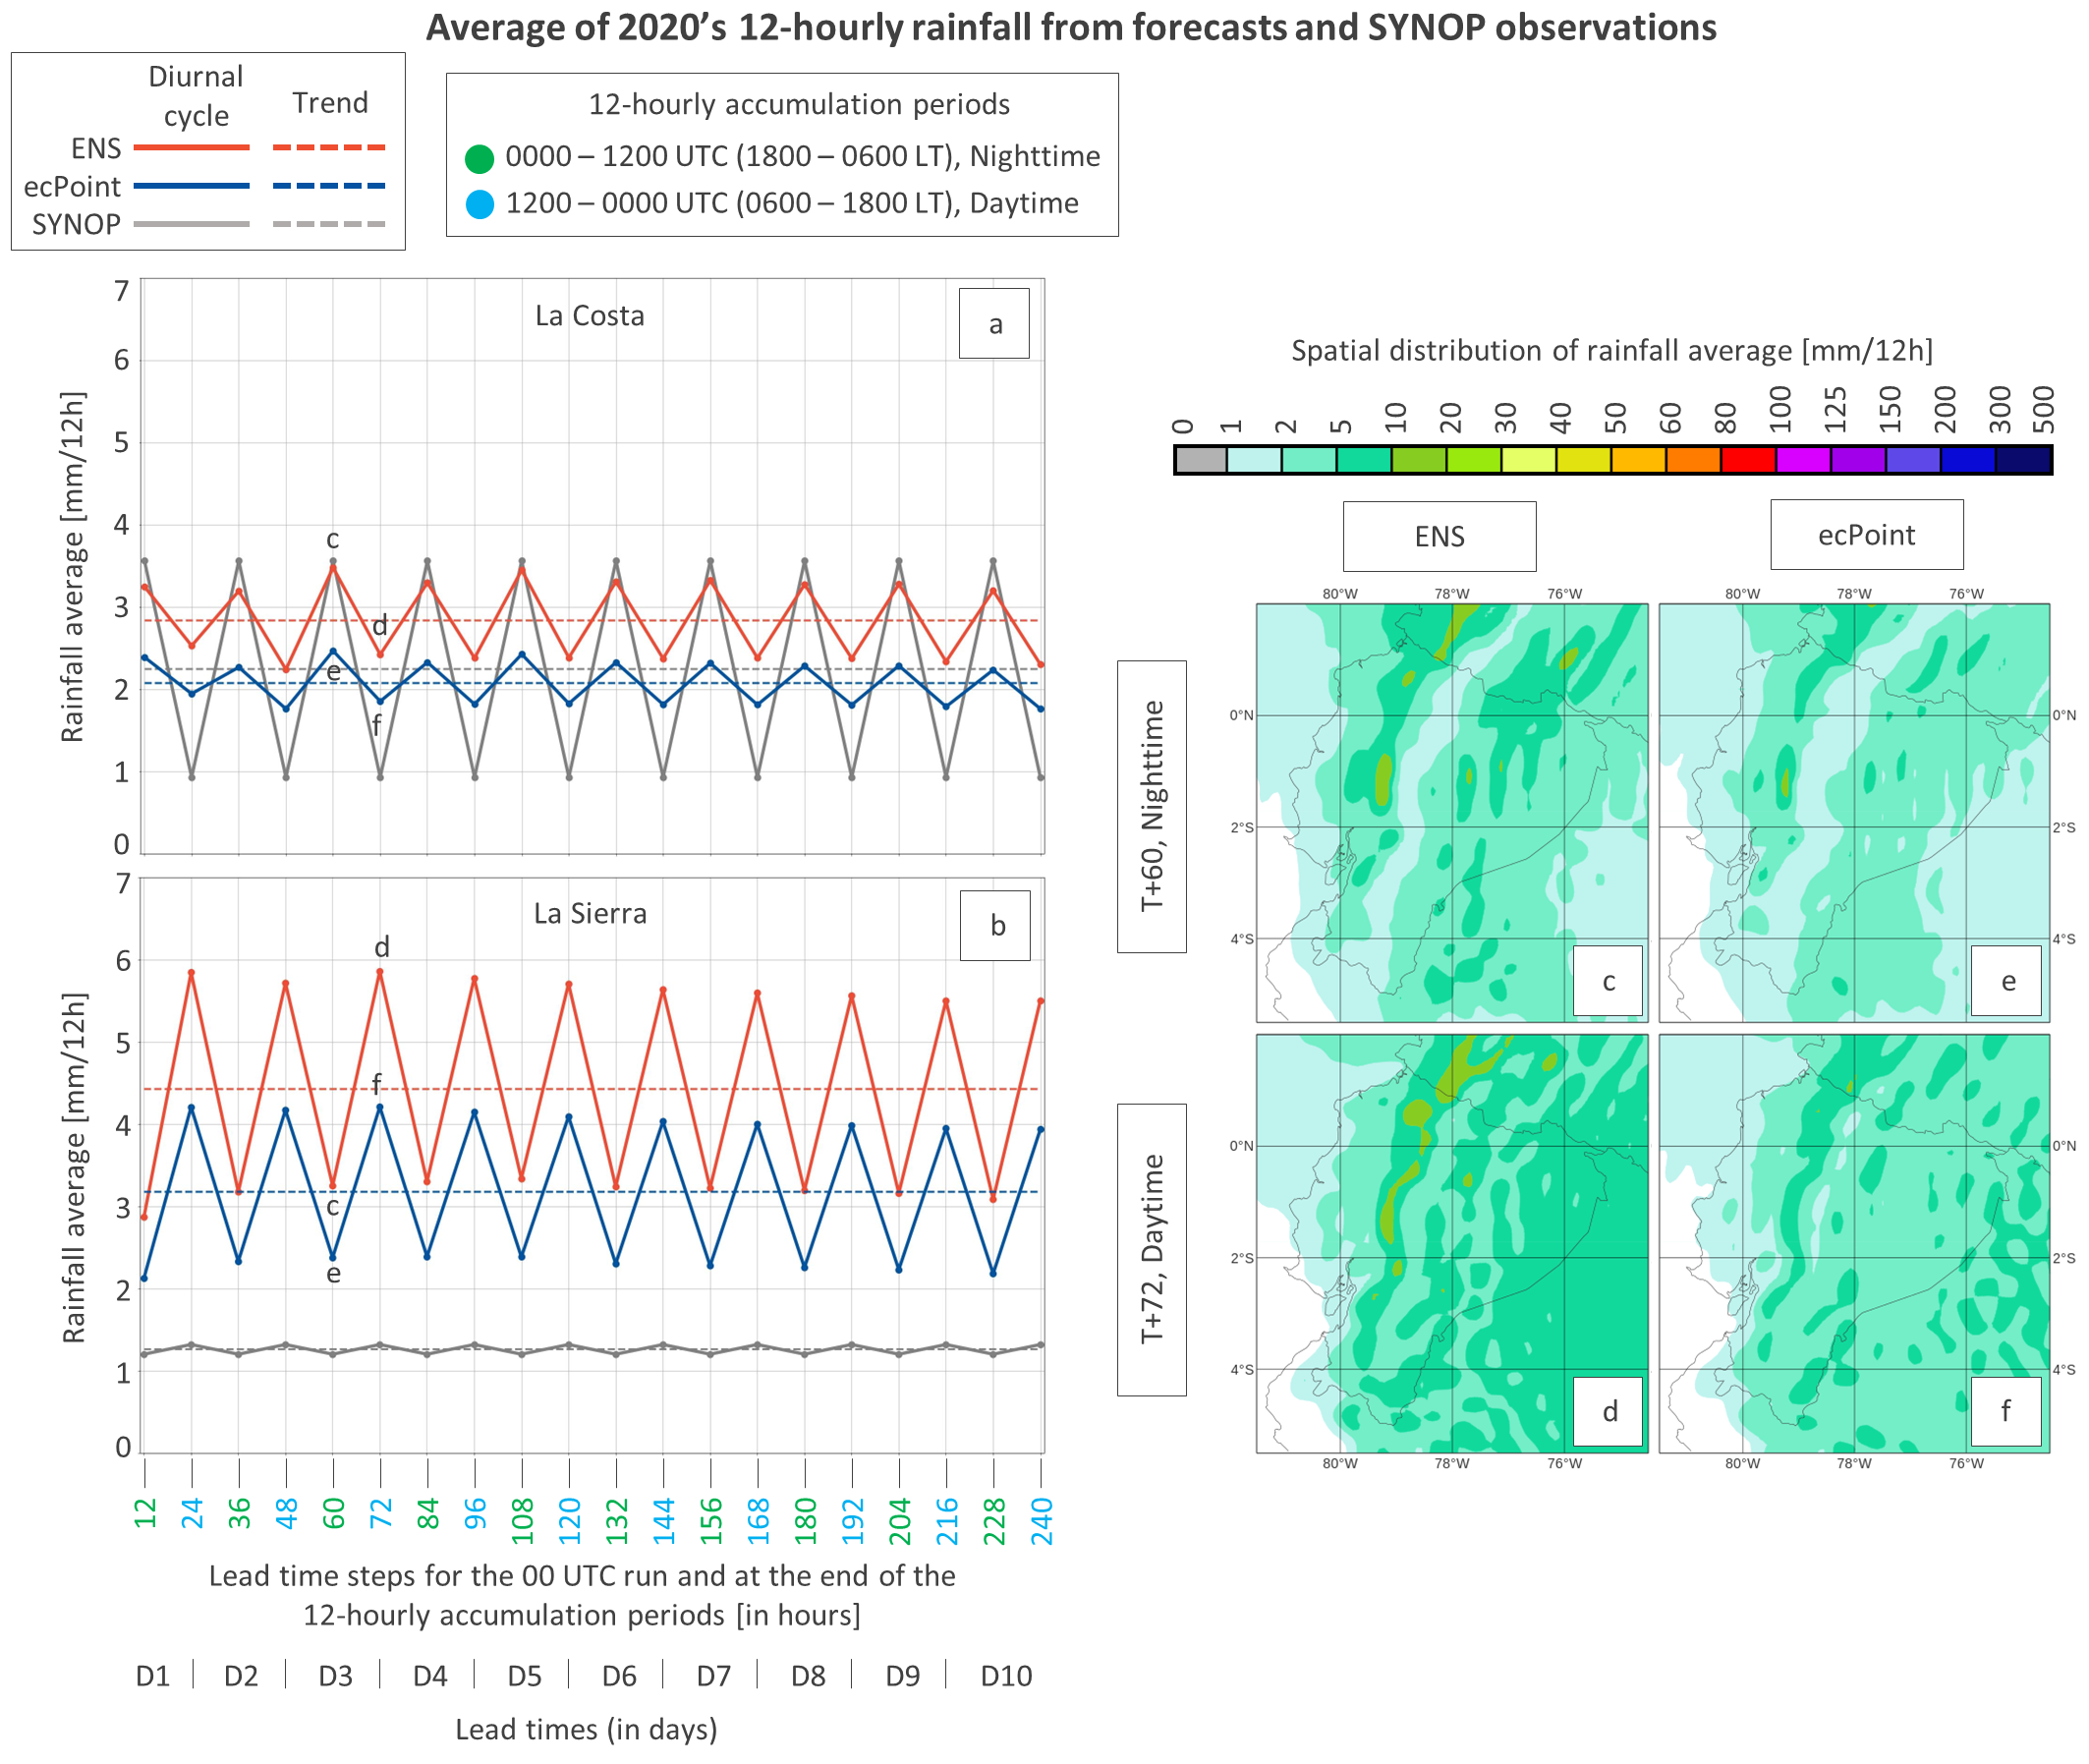
\includegraphics[width=\textwidth]{Figures/06_DATA_Annual_Average_Rainfall.png}
\caption{Panels (a) and (b) show, for “La Costa” and “La Sierra”, respectively, the 12-hourly rainfall average (continuous line) and their trend (dashed line)  as a function of forecast lead time up to day 10. SYNOP, ENS, and ecPoint are shown in grey, red, and blue, respectively. The x-axis indicates the lead time steps (in hours) at the end of the 12-hourly accumulation period. Each step is colour-coded according to the valid accumulation period (in UTC and LT) based on the 00 UTC run: the steps representing the accumulation period between 0000-1200 UTC (or 1800-0600 LT, night-time) are shown in green, while the steps representing the accumulation period between 1200-0000 UTC (or 0600-1800 LT, daytime) are shown in cyan. Panels (c) and (d) illustrate examples of a typical spatial distribution of rainfall averages, respectively, at night-time and daytime for a day 3 forecast in ENS (accumulation periods ending at steps t+60 and t+72, respectively). Panels (e) and (f) show the same but for ecPoint.}
\label{fig:Annual_Average_Rain}
\end{figure}

The ECMWF ENS consists of one control run starting from the best possible representation of unperturbed initial conditions, and 50 perturbed members starting from perturbed initial conditions (using singular vectors and a data assimilation ensemble) and stochastic model uncertainties \citep{Buizza2019}. Up to day 15, ENS forecasts are saved in the native octahedral reduced-Gaussian with a resolution of ~18 km at the equator \citep{Owens2018}. Over the period used to compute the climatology of rainfall events associated with flash flood events (1st January to 31st December 2019) and the verification period (1st January to 31st December 2020), three different model versions were run operationally at ECMWF: 45r1\footnote{www.ecmwf.int/en/forecasts/documentation-and-support/evolution-ifs/cycles/summary-cycle-45r1}  (for forecasts from 1st January to 10th June 2019), 46r1\footnote{www.ecmwf.int/en/forecasts/about-our-forecasts/evolution-ifs/cycles/summary-cycle-46r1}  (from 11th June 2019 to 12th July 2020), and 47r1\footnote{www.ecmwf.int/en/forecasts/about-our-forecasts/evolution-ifs/cycles/summary-cycle-47r1}  (from 13th July to 31st December 2020). This mismatch of model versions is unlikely to adversely affect the verification results because no significant changes were made in the physics of the rain generation mechanisms in the considered model versions.

ecPoint is a decision-tree-based statistical post-processing technique that transforms global grid-based forecasts into probabilistic point-scale forecasts \citep{Hewson2021}. The post-processing technique aims to provide forecasts that mirror observations from rain gauges by addressing the two main factors affecting the performance of the global NWP model output against point verification: systematic biases \citep{Lavers2021} and lack of information on forecast sub-grid variability \citep{Gober2008}. For each raw ENS member, ecPoint generates an ensemble of 100 point-rainfall values based on the error distributions between forecasts and observations that vary according to different weather scenarios at the grid-box level. For example, when on a grid box, the model mainly predicts large-scale rainfall with light winds, the raw model output tends to be representative of point rainfall totals within that grid box, and ecPoint generates an ensemble with a smaller spread compared to the case of mainly convective rainfall with light winds. In the latter case, many points within the grid-box are expected to show zero rainfall while very large rainfall amounts might be observed at a few points. From the current operational configuration of ENS forecasts (i.e., 51 ensemble members), the 5100 point-scale rainfall values were distilled in percentiles from the 1\textsuperscript{st} to the 99\textsuperscript{th}. ecPoint forecasts are provided in the same native grid of ENS forecasts up to day 10 lead times and in four overlapping 12-hourly accumulation periods with valid times starting at 0, 6, 12, and 18 UTC.

Figure \ref{fig:Percentiles} shows examples of the ENS and ecPoint rainfall forecasts from the 85\textsuperscript{th} and 99\textsuperscript{th} percentiles. Typically, percentiles from ecPoint lower than or equal to the 85\textsuperscript{th} percentile (Figure \ref{fig:Percentiles}\hyperref[fig:Percentiles]{c}) have lower rainfall forecast values than the ENS (Figure \ref{fig:Percentiles}\hyperref[fig:Percentiles]{a}). This is because, generally, the number of zero rainfall totals is larger in ecPoint than in ENS. This is a bias correction applied to the rainfall forecasts by ecPoint, as ENS tends to overpredict small rainfall totals \citep{Haiden2023}. On the contrary, big percentiles (typically above the 90\textsuperscript{th} percentile) tend to show larger rainfall totals on ecPoint than in ENS. This can be noticed in Figure \ref{fig:Percentiles}\hyperref[fig:Percentiles]{d} by the overall domination of the orange colour (i.e., rainfall totals between 50 and 80 mm/12h) compared to Figure \ref{fig:Percentiles}\hyperref[fig:Percentiles]{b} where the dominant colour is green (i.e., rainfall totals between 10 and 30 mm/12h).  It is noteworthy that ecPoint does not always increase the amounts of the rainfall forecasts.  In certain parts of “La Costa”, the rainfall totals in ecPoint are lower than those in ENS because the post-processing considered that the raw rainfall forecasts might be overpredicted under the predicted grid-box weather type. While \cite{Hewson2021} showed with a global objective verification analysis over a one-year period that, up to medium-range lead times (i.e., day 10 forecasts), ecPoint provides forecasts for point-scale rainfall with better reliability and discrimination ability than ENS, especially for extremes, it is interesting to compare how ENS and ecPoint perform in the prediction of rainfall in Ecuador. Figure \ref{fig:Annual_Average_Rain}\hyperref[fig:Annual_Average_Rain]{a} and \ref{fig:Annual_Average_Rain}\hyperref[fig:Annual_Average_Rain]{b} shows 2020’s 12-hourly rainfall average from SYNOP observations (in grey) and forecasts (ENS in red and ecPoint in blue), respectively, for la Costa“ and “La Sierra”. There is no degradation in performance with lead times up to day 10, and both forecasting systems reproduce the fact that Ecuador’s rainfall is affected by a diurnal cycle. However, neither ENS nor ecPoint can correctly represent the peaks and troughs of the diurnal cycle of rainfall. While in “La Costa” ENS represents the rainfall peaks during night-time exceptionally well, it significantly overestimates the rainfall over daytime (Figure \ref{fig:Annual_Average_Rain}\hyperref[fig:Annual_Average_Rain]{a}). With the aim of reducing the daytime bias, ecPoint unnecessarily reduces the night-time rainfall and reduces the overall amplitude of the rainfall’s diurnal cycle. This is because for 12-hourly rainfall, ecPoint makes no distinction between rainfall at different times of the day. Figure \ref{fig:Annual_Average_Rain}\hyperref[fig:Annual_Average_Rain]{c} shows how ENS predicts most of the rainfall during night-time on the western slopes of the Andes, while ecPoint tends to remove most of the rainfall, leaving the rainfall in the Pacific coast mostly unchanged (Figure \ref{fig:Annual_Average_Rain}\hyperref[fig:Annual_Average_Rain]{e}). During the daytime, the ENS still produces high amounts of rainfall, primarily on the western slopes of the Andes (Figure \ref{fig:Annual_Average_Rain}\hyperref[fig:Annual_Average_Rain]{d}). ecPoint applies a general reduction in rainfall in “La Costa” (Figure \ref{fig:Annual_Average_Rain}\hyperref[fig:Annual_Average_Rain]{f}). It can be observed that ecPoint’s overall rainfall average (blue dashed line in Figure \ref{fig:Annual_Average_Rain}\hyperref[fig:Annual_Average_Rain]{a}) is closer than that of ENS (red dashed line) to the observed average (grey dashed line). In “La Sierra” (Figure \ref{fig:Annual_Average_Rain}\hyperref[fig:Annual_Average_Rain]{b}) although again ecPoint’s overall rainfall average is closer than ENS to the observed average, both forecasts significantly overestimate the absolute values of daytime and night-time rainfall and the amplitude of the observed rainfall diurnal cycle. In Figure \ref{fig:Annual_Average_Rain}\hyperref[fig:Annual_Average_Rain]{c} to Figure \ref{fig:Annual_Average_Rain}\hyperref[fig:Annual_Average_Rain]{f}, it can be observed that ecPoint applies a reduction in the rainfall forecasts generalized over the entire region. 


%%%%%%%%%%%%%%%%%%%%%%%%%%%%%%%%%%%%%%%%%%%%%%%%%%%%%%%%%%%%%

\section{Methods}
\label{sec:Methods}

\begin{figure}
\centering
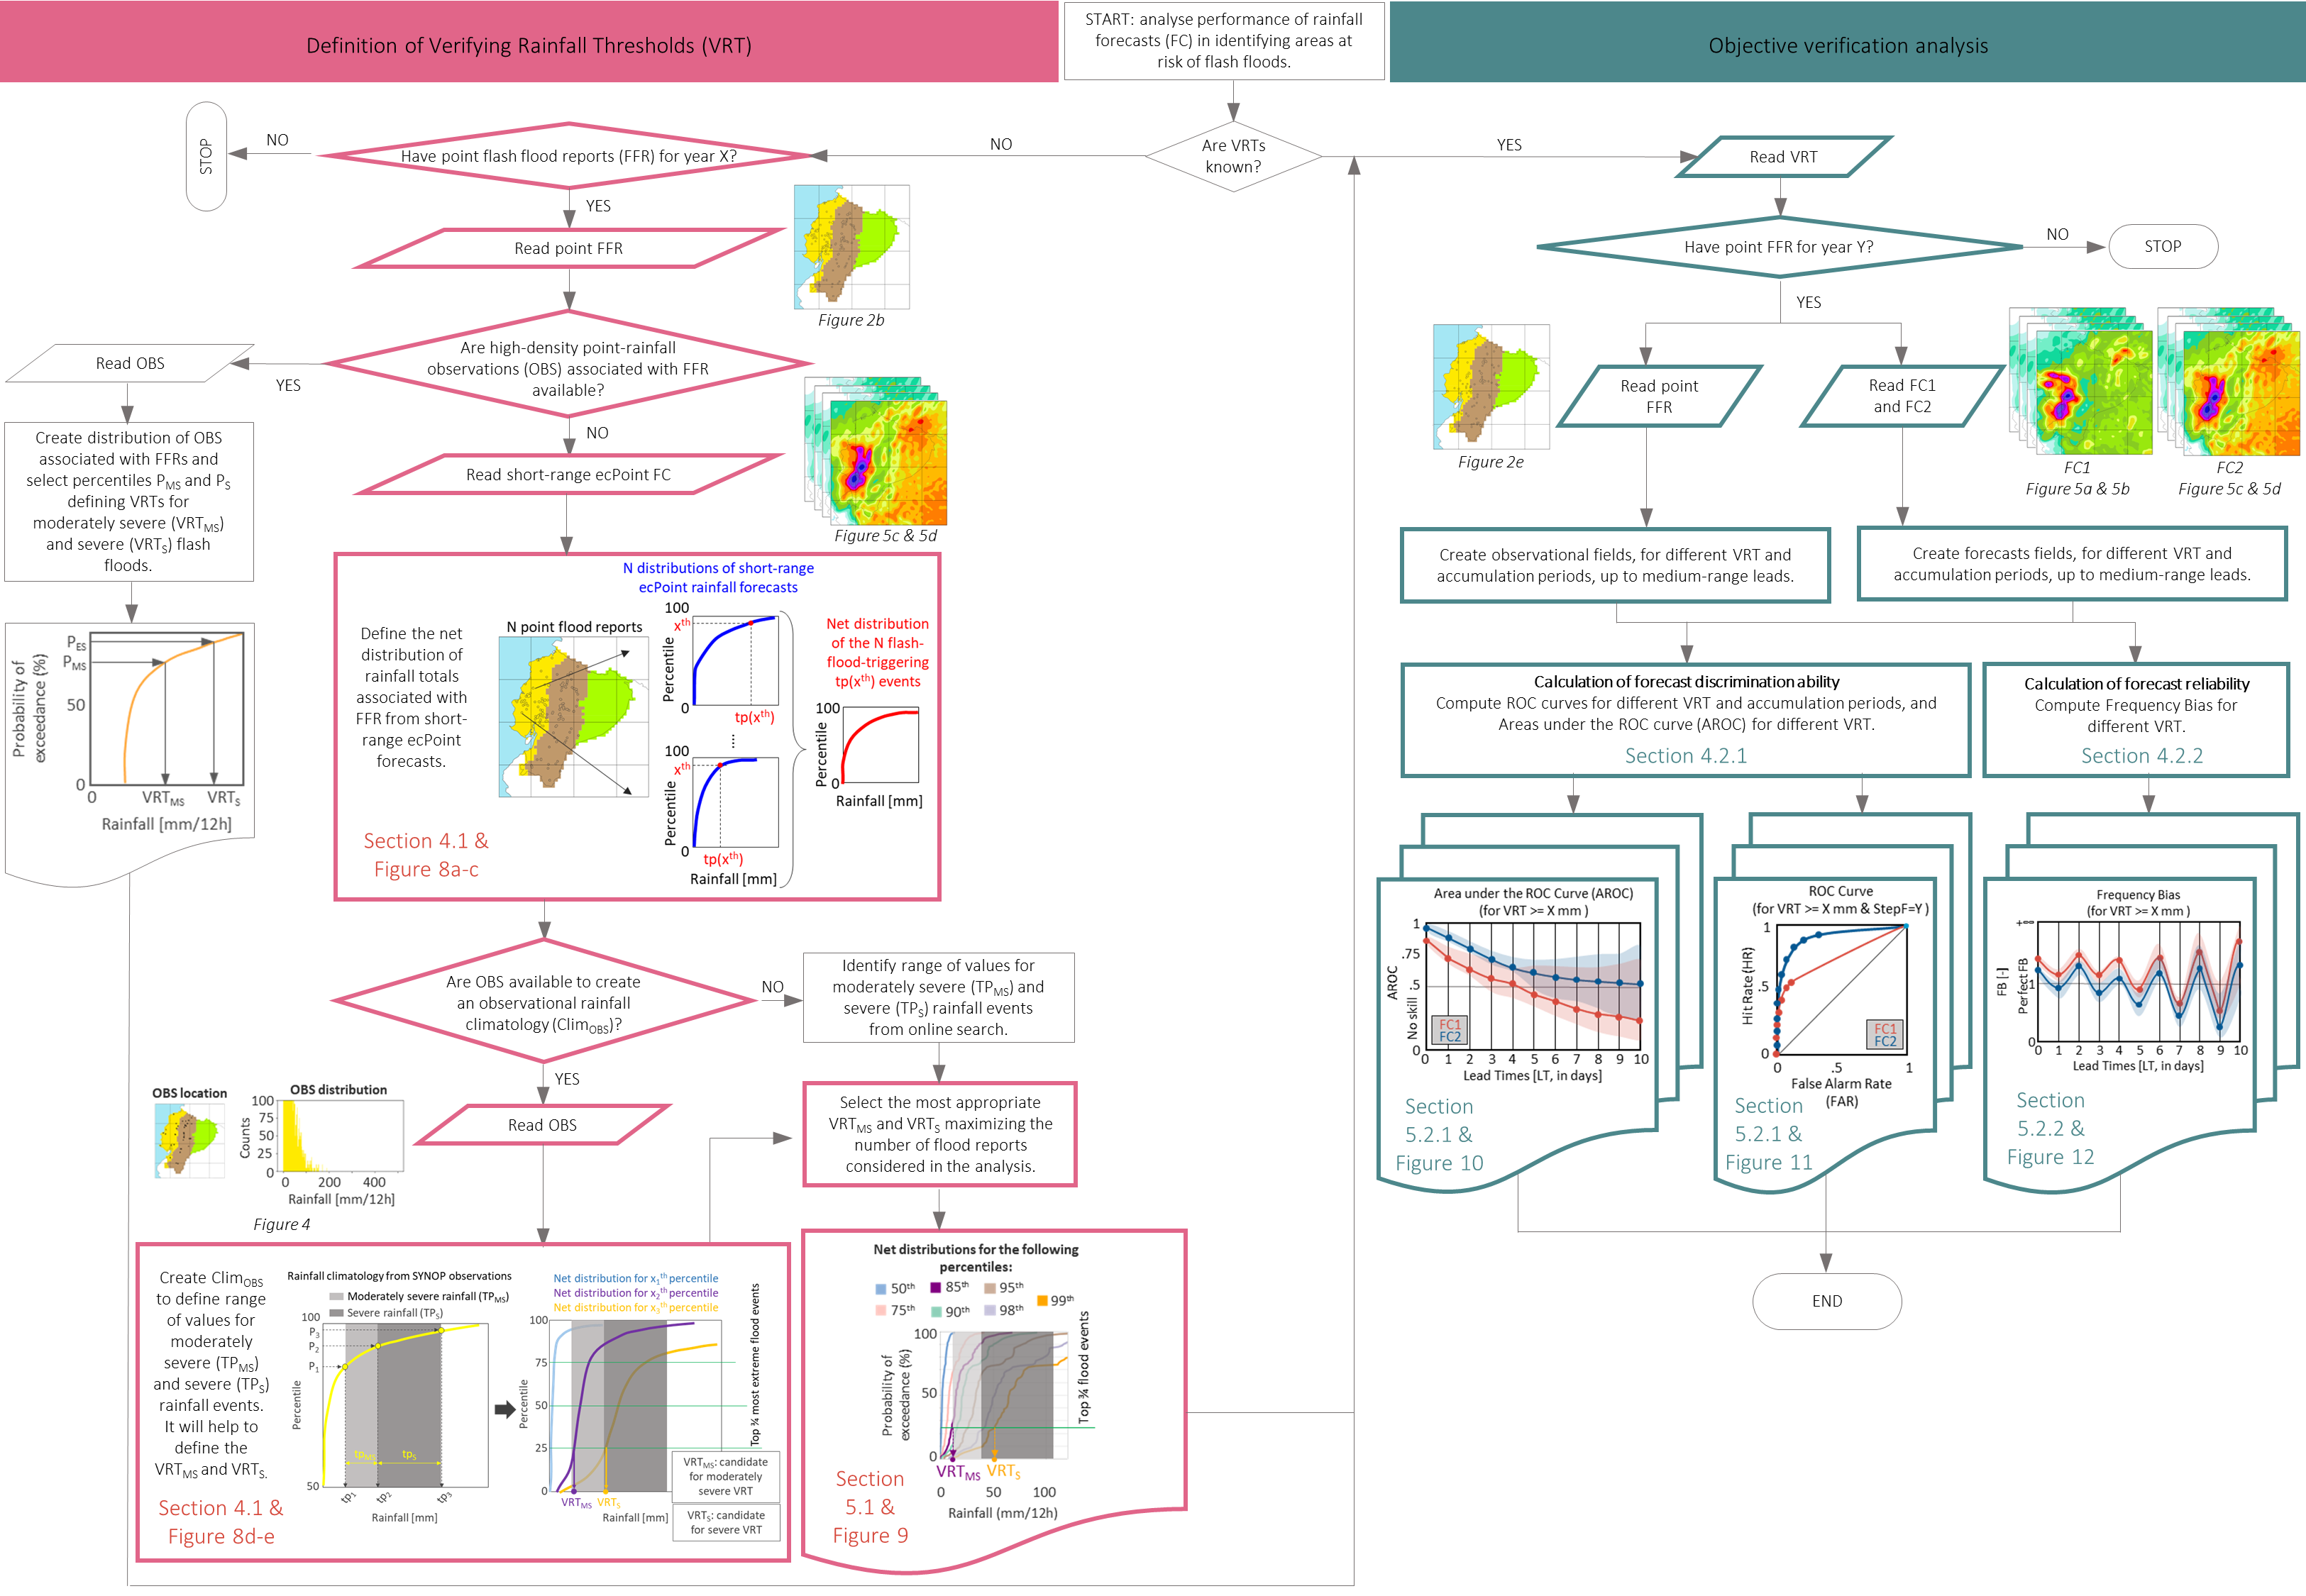
\includegraphics[width=1.3\textwidth, angle=90]{Figures/07_METHODS_Flow_Chart.png}
\caption{Flowchart of the general methodological steps to determine the verifying rainfall thresholds (pink area) and to assess the forecasts’ performance in identifying areas at risk of flash floods (green area). The coloured boxes highlight the actual steps taken in this study.}
\label{fig:Flow_Chart}
\end{figure}

The two main attributes of any probabilistic forecasting system are reliability and discrimination ability, which together determine the performance of the system \citep{Jolliffe2011}. Reliability and discrimination ability are defined for events exceeding a certain rainfall threshold (e.g., 50 mm/12h). Hereafter, this rainfall threshold will be referred to as verifying rainfall threshold (VRT). Reliability measures whether the chosen VRT is predicted with a probability that equals the average frequency at which such an event is observed. Discrimination measures the ability of the forecasting system to distinguish situations that lead to events exceeding the VRT or not. This study faced two main challenges. Since they were not known a priori, the first challenge was to define the magnitude (in mm) of flash-flood-triggering rainfall events to be used as the VRT values in the objective verification analysis. The pink area in the flowchart in Figure \ref{fig:Flow_Chart} provides a graphical representation of the steps described in section \ref{sec:Methods_VRT} to define the VRT values. The second challenge relates to the objective verification analysis. First, due to the intrinsic characteristics of the observational dataset, it was not possible to define univocally observational yes- and no-events. Second, since the probabilistic rainfall forecasts were converted into binary predictions (yes- or no-event), reliability in the usual probabilistic sense cannot be computed. The frequency bias was then calculated to determine the overall reliability of the system, indicating whether the system is, on average, under- or over-forecasting the occurrence of flash flood events. The green area in the flowchart in 
Figure \ref{fig:Flow_Chart} provides the graphical representation of the steps taken in this study to conduct the objective verification, whose details are described in section \ref{sec:Methods_OV}.

\subsection{Definition of the verifying rainfall thresholds (VRT)}
\label{sec:Methods_VRT}

\begin{figure}
\centering
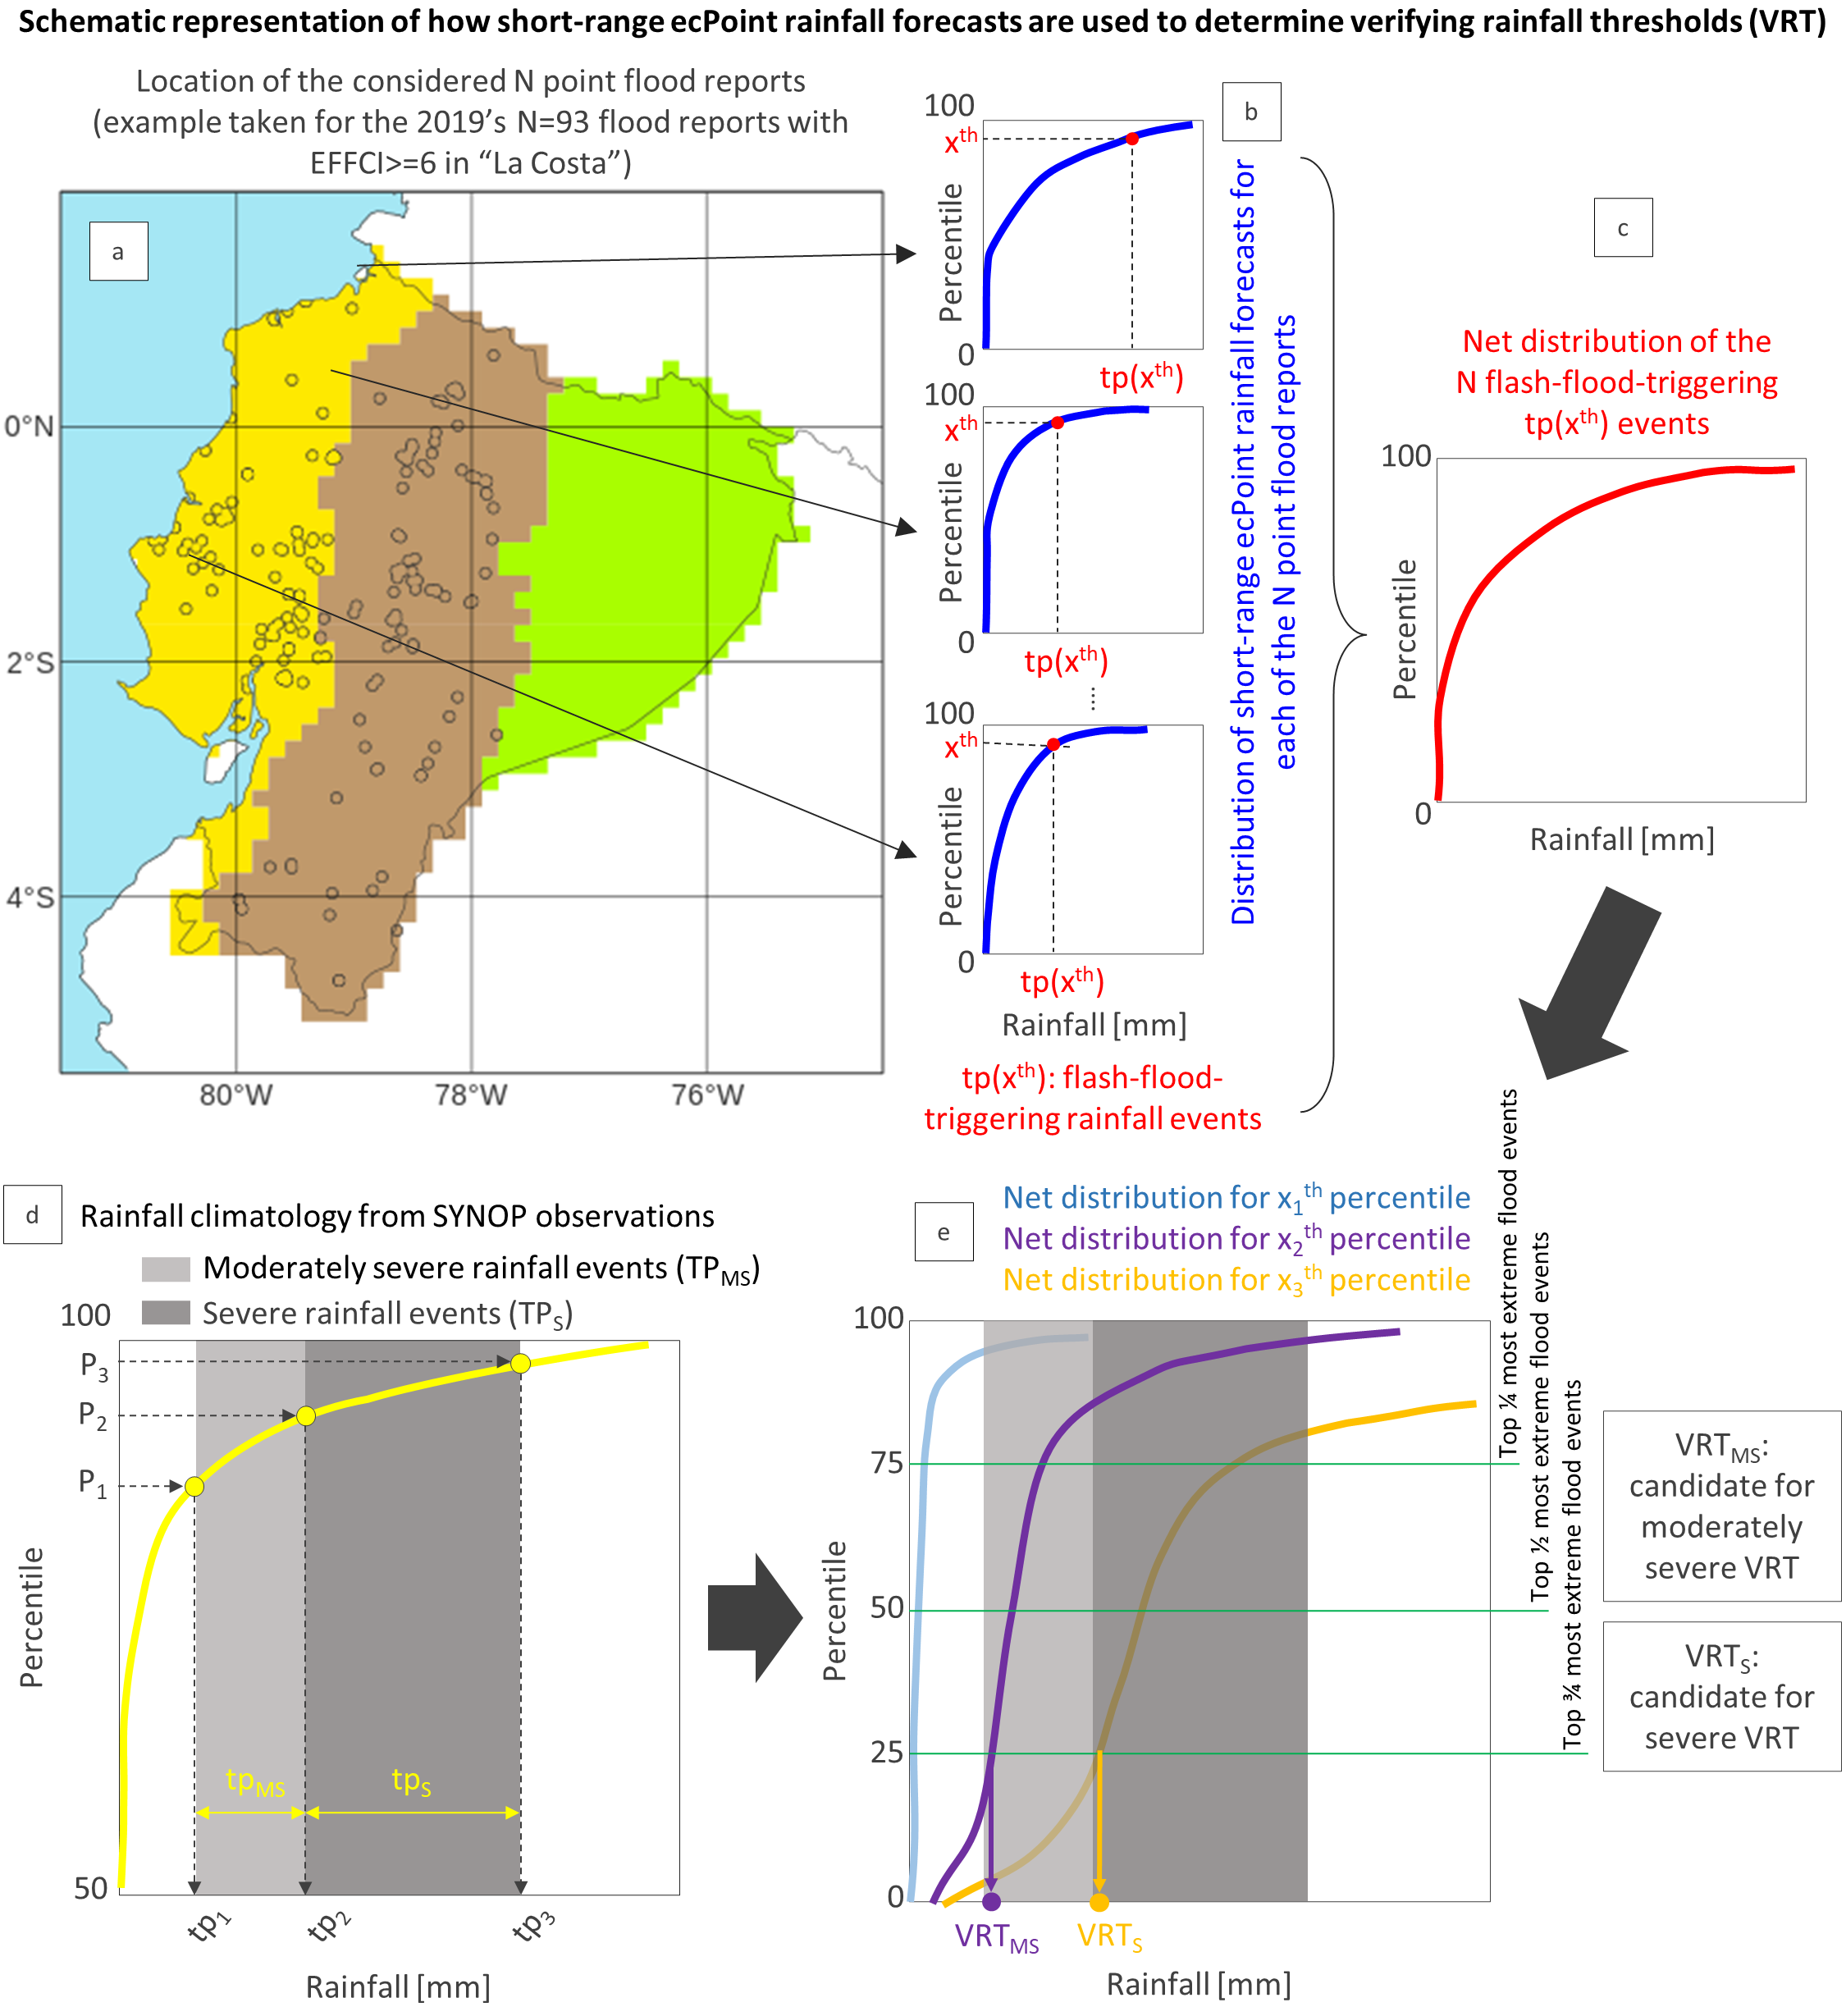
\includegraphics[width=0.8\textwidth]{Figures/08_METHODS_VRTs.png}
\caption{Schematic representation of how short-range ecPoint rainfall forecasts are used to determine verifying rainfall thresholds (VRT) using 2019's N=93 point flood reports with EFFCI$\geq$6 in “La Costa” as an example (see Figure \ref{fig:PointFR_Maps}\hyperref[fig:PointFR_Maps]{b} and Table \ref{table:CountFR_EFFCI}). Panel (a) shows the location of the N point flood reports. Panel (b) shows examples of possible distributions of short-range ecPoint rainfall forecasts associated with each of the N point flood reports (in blue). If a sufficiently large x\textsuperscript{th} percentile is considered in each distribution, the corresponding tp(x\textsuperscript{th}) values can be regarded as flash-flood-triggering rainfall events (in red). Panel (c) displays the net distribution (in red) of the N flash-flood-triggering rainfall events. In the example, only one distribution is shown. However, as many distributions as desired can be created by considering different percentiles. Panel (d) shows the rainfall climatology (in yellow, as this example refers to “La Costa”) built from SYNOP observations. The percentiles P\textsubscript{1} and P\textsubscript{2}, and the corresponding rainfall values tp\textsubscript{1} and tp\textsubscript{2}, define the range of moderately severe rainfall values (tp\textsubscript{MS}), whose width is visually highlighted by the light grey rectangle. The percentiles P\textsubscript{2} and P\textsubscript{3}, and the corresponding rainfall values tp\textsubscript{2} and tp\textsubscript{3}, define the range of severe rainfall values (tp\textsubscript{S}), whose width is visually highlighted by the dark grey rectangle. Using the two rainfall ranges and a pre-established top fraction of the most extreme N flood reports, panel (e) illustrates how candidates for moderately severe VRT\textsubscript{MS} and severe VRT\textsubscript{S} are determined when a series of net distributions of flash-flood-triggering rainfall events are available.}
\label{fig:Methods_VRT}
\end{figure}

\begin{figure}
\centering
\captionof{table}{Day 1 ecPoint-Rainfall forecasts used to define the verifying rainfall thresholds (VRT).  }
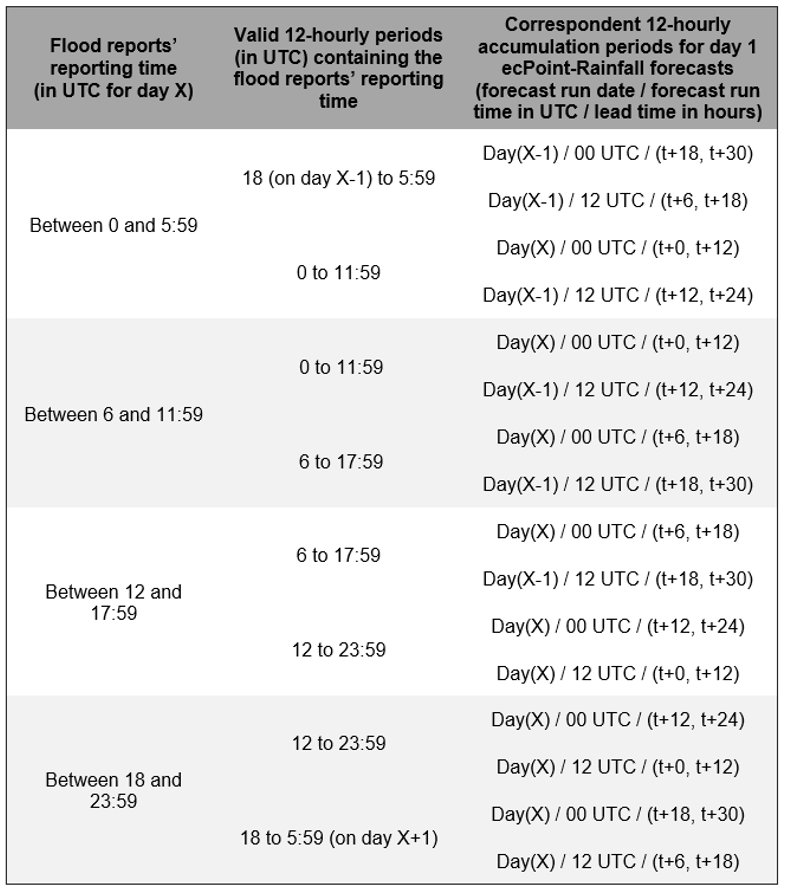
\includegraphics[width=0.5\textwidth]{Tables/02_FC_ProxyOBS.png}
\label{table:FC_ProxyOBS}
\end{figure}

If not known a priori, VRT magnitudes can be defined in several ways (see Figure \ref{fig:Flow_Chart}, pink area “Definition of VRT”). If point rainfall observations are available (e.g., rain gauges or radars), one can create the distribution of the observed flash-flood-triggering rainfall totals. VRT values would then correspond to the specific percentiles of the distribution. The higher the percentile, the higher the magnitude of the VRT, and the higher the severity level of flash flood events considered in the objective verification analysis would be. This approach requires high-density rainfall observations, in both space and time, to capture the extreme (localised) rainfall totals that trigger flash floods \citep{Haiden2016, RamosFilho2021}. In the absence of a suitable observational network (for example, in Ecuador, no high-density in-situ 12-hourly rainfall observations were available as shown in Figure \ref{fig:Descriptio_SYNOP}\hyperref[fig:Descriptio_SYNOP]{a} and Figure \ref{fig:Descriptio_SYNOP}\hyperref[fig:Descriptio_SYNOP]{b}), the VRT values can be defined only from gridded rainfall products such as reanalysis e.g., ERA5 \citep{Hersbach2020}, reforecasts \citep{Hamill2006}, or blended rainfall observations provided on a grid such as MSWEP \citep{Beck2019} or GPCP \citep{Adler2018}. These datasets tend to, however, underestimate rainfall extremes because of their coarse resolution \citep{Tapiador2019a}.

In the absence of more suitable point-scale datasets, this study proposes a methodology for creating a synthetic distribution of flash-flood-triggering rainfall events using short-range ecPoint rainfall forecasts (Figure \ref{fig:Flow_Chart}, pink area). The synthetic distribution will also be compared with the distribution obtained from the low-resolution point-rainfall observations available in Ecuador. At short-range leads, the ecPoint rainfall realisations can be considered proxies for point rainfall observations within the grid boxes \citep{Hewson2021}. Each of the N flood reports is associated with ecPoint rainfall forecasts from the nearest grid box (Figure \ref{fig:Methods_VRT}\hyperref[fig:Methods_VRT]{a}). At each forecast run, two 12-hourly accumulation periods span each flood report’s reporting time (see the first and second columns of \ref{table:FC_ProxyOBS}, so a distribution of 396 ecPoint rainfall realisations (that is, 99 ecPoin rainfall values × 2 accumulation periods × 2 runs) can be built for each flood report (blue lines in Figure \ref{fig:Methods_VRT}\hyperref[fig:Methods_VRT]{b}). Owing to the high number of forecast realizations per flood report, only one year of short-range forecasts is sufficient to define the VRT values. The rainfall value (tp) associated with the X\textsuperscript{th} percentile of the distribution (red dots in Figure \ref{fig:Methods_VRT}\hyperref[fig:Methods_VRT]{b}) characterizes a certain level of severity for a flash-flood-triggering rainfall event. The net distribution of the N tp(x\textsuperscript{th}) values (red distribution in Figure \ref{fig:Methods_VRT}\hyperref[fig:Methods_VRT]{c}) represents the distribution of flash-flood-triggering rainfall events. Several reasonably high X\textsuperscript{th} percentiles, eg., the 50\textsuperscript{th}, 75\textsuperscript{th}, 85\textsuperscript{th}, 90\textsuperscript{th}, 95\textsuperscript{th}, 98\textsuperscript{th}, and 99\textsuperscript{th}, were tested to exclude low rainfall totals from the analysis as they would have unlikely been the drivers of any flash flood event. To choose which X\textsuperscript{th} percentiles retain in the analysis, two severity categories were defined from the distribution of flash-flood-triggering rainfall events computed from a time series of 10 years SYNOP observations (Figure \ref{fig:Methods_VRT}\hyperref[fig:Methods_VRT]{d}): moderately severe (MS) between P\textsubscript{1} = 95\textsuperscript{th} and P\textsubscript{2} = 99\textsuperscript{th} percentiles, and severe (S) between P\textsubscript{2} = 99\textsuperscript{th} and P\textsubscript{3} = 99.99\textsuperscript{th} percentiles. The values of the percentiles P\textsubscript{1}, P\textsubscript{2}, and P\textsubscript{3} were chosen considering best practices for the definition of thresholds found in the literature \citep{Zsoter2020, Mitheu2023} and \cite{Hewson2021} recommendations for defining extremes in ecPoint rainfall forecasts. Finally, the corresponding VRT\textsubscript{MS} and VRT\textsubscript{S} were defined by deciding how many flood reports would like to be retained in the analysis, for example, the top 1/4, 1/2, or 3/4 (Figure \ref{fig:Methods_VRT}\hyperref[fig:Methods_VRT]{d}). While such decision can be seen as arbitrary, it depends on the number of reports available at the beginning of the analysis, so that a reasonable number of events are maintained to produce robust statistics. In this study, the top 3/4 flood events were maintained due to the initial small number of events in the database (Table \ref{table:CountFR_EFFCI}). Separate VRT values were calculated for “La Costa” and “La Sierra” to capture their hydro-climatological regimes. 

\subsection{Objective verification to assess the rainfall forecasts’ performance in the identification of areas at flash flood risk}
\label{sec:Methods_OV}

\subsubsection{Assessment of forecasts’ discrimination ability: Receiver Operating Characteristic (ROC) curves and Area Under the ROC curve (AROC)}

\begin{figure}
\centering
\captionof{table}{Definition of the four quadrants in a contingency table.}
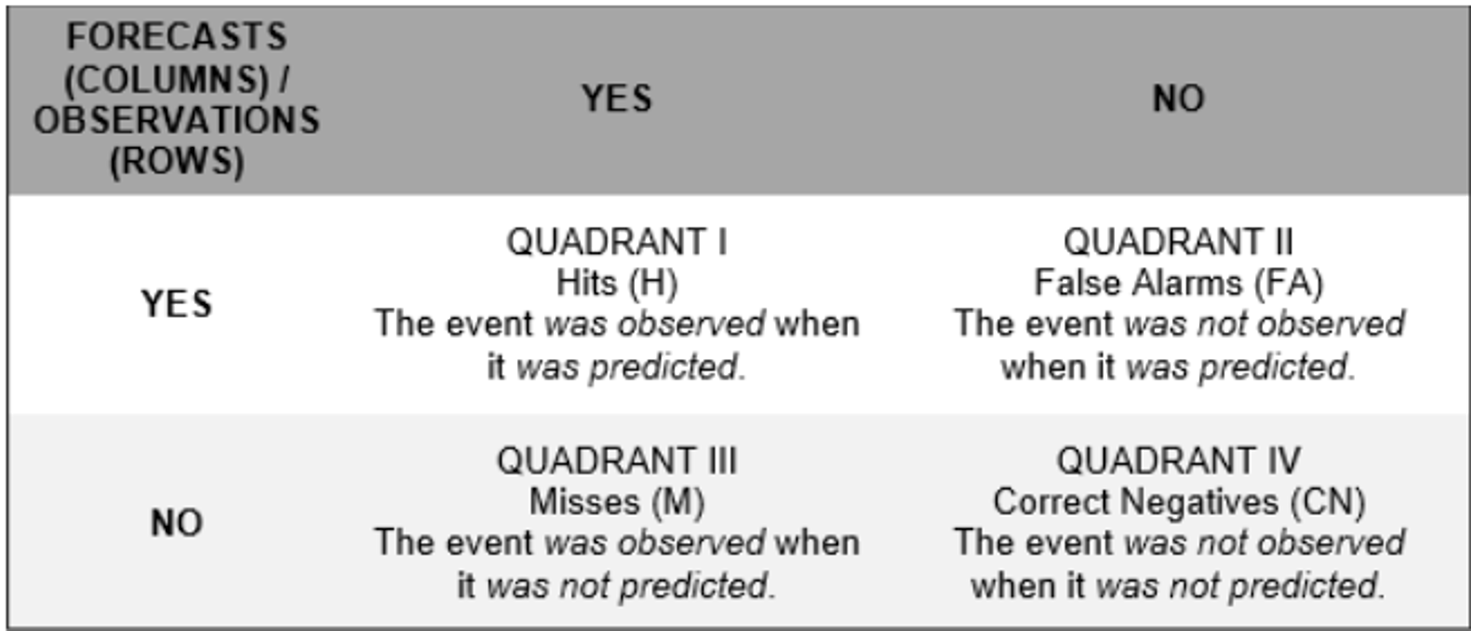
\includegraphics[width=0.5\textwidth]{Tables/03_CT.png}
\label{table:CT}
\end{figure}

This study used the Receiver Operating Characteristic (ROC) curve and the area under the ROC curve (AROC) to estimate and compare the discrimination ability of ENS and ecPoint rainfall forecasts in the prediction of areas at risk of flash floods \citep{Jolliffe2011}. ROC curves were constructed using a 2 × 2 contingency table that quantifies the hits (H), misses (M), false alarms (FA), and correct negatives (CN) that occur when action is advised based on the VRT exceeding each sampled probability threshold (see Table \ref{table:CT} for the definition of the constituting elements of the contingency table). Correspondent hit rates (HR) and false alarm rates (FAR) can be then computed, respectively, from equations (\ref{eq:HR}) and (\ref{eq:FAR}):

\begin{equation}
HR = \frac{H}{H+M} \quad \text{[values between 0 and 1]}
\label{eq:HR}
\end{equation}

\begin{equation}
FAR = \frac{FA}{FA+CN} \quad \text{[values between 0 and 1]}
\label{eq:FAR}
\end{equation}

For each sampled probability threshold, the ROC curves map HRs on the Y-axis against FARs on the X-axis. The location of the ROC curve in the graph and the geometrical area under the ROC curve (AROC) determine the discrimination ability of the forecasting system. Perfect discrimination is obtained when only HRs grow, whereas the FARs always remain equal to zero. This is represented by an ROC curve that rises from the bottom left corner (0,0) along the Y-axis to the top-left corner (0,1) and moves straight to the top-right corner (1,1). In this case, the AROC was equal to 1.  When the forecasting system has no discriminatory ability (i.e., it does not provide any additional information beyond climatological predictions), the HRs and FARs grow at the same rate. Therefore, the ROC curve lies along the diagonal of the graph, and the AROC is equal to 0.5.
How ROC curves are built and AROCs are computed has a significant impact on the interpretation of the results. To ensure that the ROC curves are as complete as possible, probability thresholds are determined using the full discretization available in the ensemble, rather than using fixed percentage bins \citep{Bouallegue2022}. Hence, ROC curves for ENS and ecPoint were constructed with 51 and 99 points, respectively. No curve fitting was used to build or complete the ROC curves, and straight lines were drawn between consecutive points in the graph, as well as the last meaningful point of the ROC curve and the top-right corner \citep{Bouallegue2022}. Moreover, AROCs are computed using the trapezoidal approximation, which simply sums the areas of single trapeziums formed by the straight lines between the ROC’s consecutive points. As a result, ROC curves for high VRT values might cluster on the bottom left corner of the graph, and if built with fewer points, they might look incomplete, and AROCs might result smaller. However, this approach focuses on the analysis of “real” and not on the “potential” discrimination ability of rainfall forecasts. The percentile bootstrapping technique was applied to evaluate whether the differences between the AROC for ENS and ecPoint were significant \citep{DiCiccio1996}. Sampling with replacement with 10,000 replicates and 95\% confidence intervals were considered.

Populating the contingency tables (Table \ref{table:CT}) is one of the challenges of this objective verification analysis. Stationary observations (i.e., provided by instruments installed at a specific location, e.g., rain gauges) provide time series that record both yes- and non-events at the location where the instrument was installed. Thus, all four elements in the contingency table can be quantified. Non-stationary observations record only yes-events at the location where the events occurred. As a result, it is impossible to answer the question “if there are no reports in an area, is it because an event happened, but nobody reported it, or because there was no event to report?”. Some studies verify only yes-events with the caveat that only quadrants I (i.e., hits) and III (i.e., misses) of the contingency table can be populated \citep{Robbins2018}. Instead, this study followed the method proposed by \cite{Tsonevsky2018}, which allows to populate all quadrants of the contingency table. This method assumes that a non-report corresponds to a non-event. Because of the high-impact nature of the event and the care used to create the observational flood database, this assumption was also considered valid for this study. Observational fields are built by assigning 1 to grid-boxes containing at least one flood report (i.e., observational yes-event); otherwise, a value of 0 is assigned (i.e., observational non-event). Forecast fields are built by assigning a value of 1 to those grid-boxes where the considered VRT is exceeded with a considered probability threshold (i.e., forecast yes-event); otherwise, the grid boxes are assigned a value of 0 (i.e., forecast non-event). The 2X2 contingency tables are built by examining overlapping grid boxes in correspondent observational and forecast fields; when both grid boxes are assigned a value of 1 or 0, they count as H and CN, respectively. When a grid box in the observational field is assigned a value of 1, and the corresponding grid box in the forecast field is assigned a value of 0, it counts as M. It counts as a false alarm (FA) if the opposite occurs.

\subsubsection{Assessment of forecasts’ calibration: Frequency Bias (FB)}
The frequency bias was used to evaluate the overall reliability of ENS and ecPoint rainfall forecasts in the prediction of areas at risk of flash floods. For each lead time, the frequency bias was determined by dividing the total number of ensemble members exceeding the considered VRT by the product of the number of ensemble members and the total number of instances when a flash flood was observed. Equation (\ref{eq:FB}) was used to compute the FB:

\begin{equation}
FB = \frac{\sum_{i=1}^{M} \sum_{j=1}^{N} \text{n. ensemble members exceeding VRT}}{\left(\text{n. ensemble members}\right) \times \left(\sum_{i=1}^{M} \sum_{j=1}^{N} \text{n. instances when a flash flood was observed}\right)} 
\label{eq:FB}
\end{equation}

FB values range from 0 to $+\infty$. FB=1 indicates perfect calibration. Scores greater and smaller than 1 indicate, respectively, that the forecasting system over- and under-predicts the observed events. It is worth noting that FB measures the overall ratio of forecast events to observed events and is not a measure of forecast skill. As such, it can provide a score of 1 when there are compensating errors. It can also be observed that a forecasting system appears to overestimate the observed number of events if the observed events are heavily underreported.

%%%%%%%%%%%%%%%%%%%%%%%%%%%%%%%%%%%%%%%%%%%%%%%%%%%%%%%%%%%%%

\section{Results}
\label{sec:Results}

\subsection{Verifying rainfall thresholds}

\begin{figure}
\centering
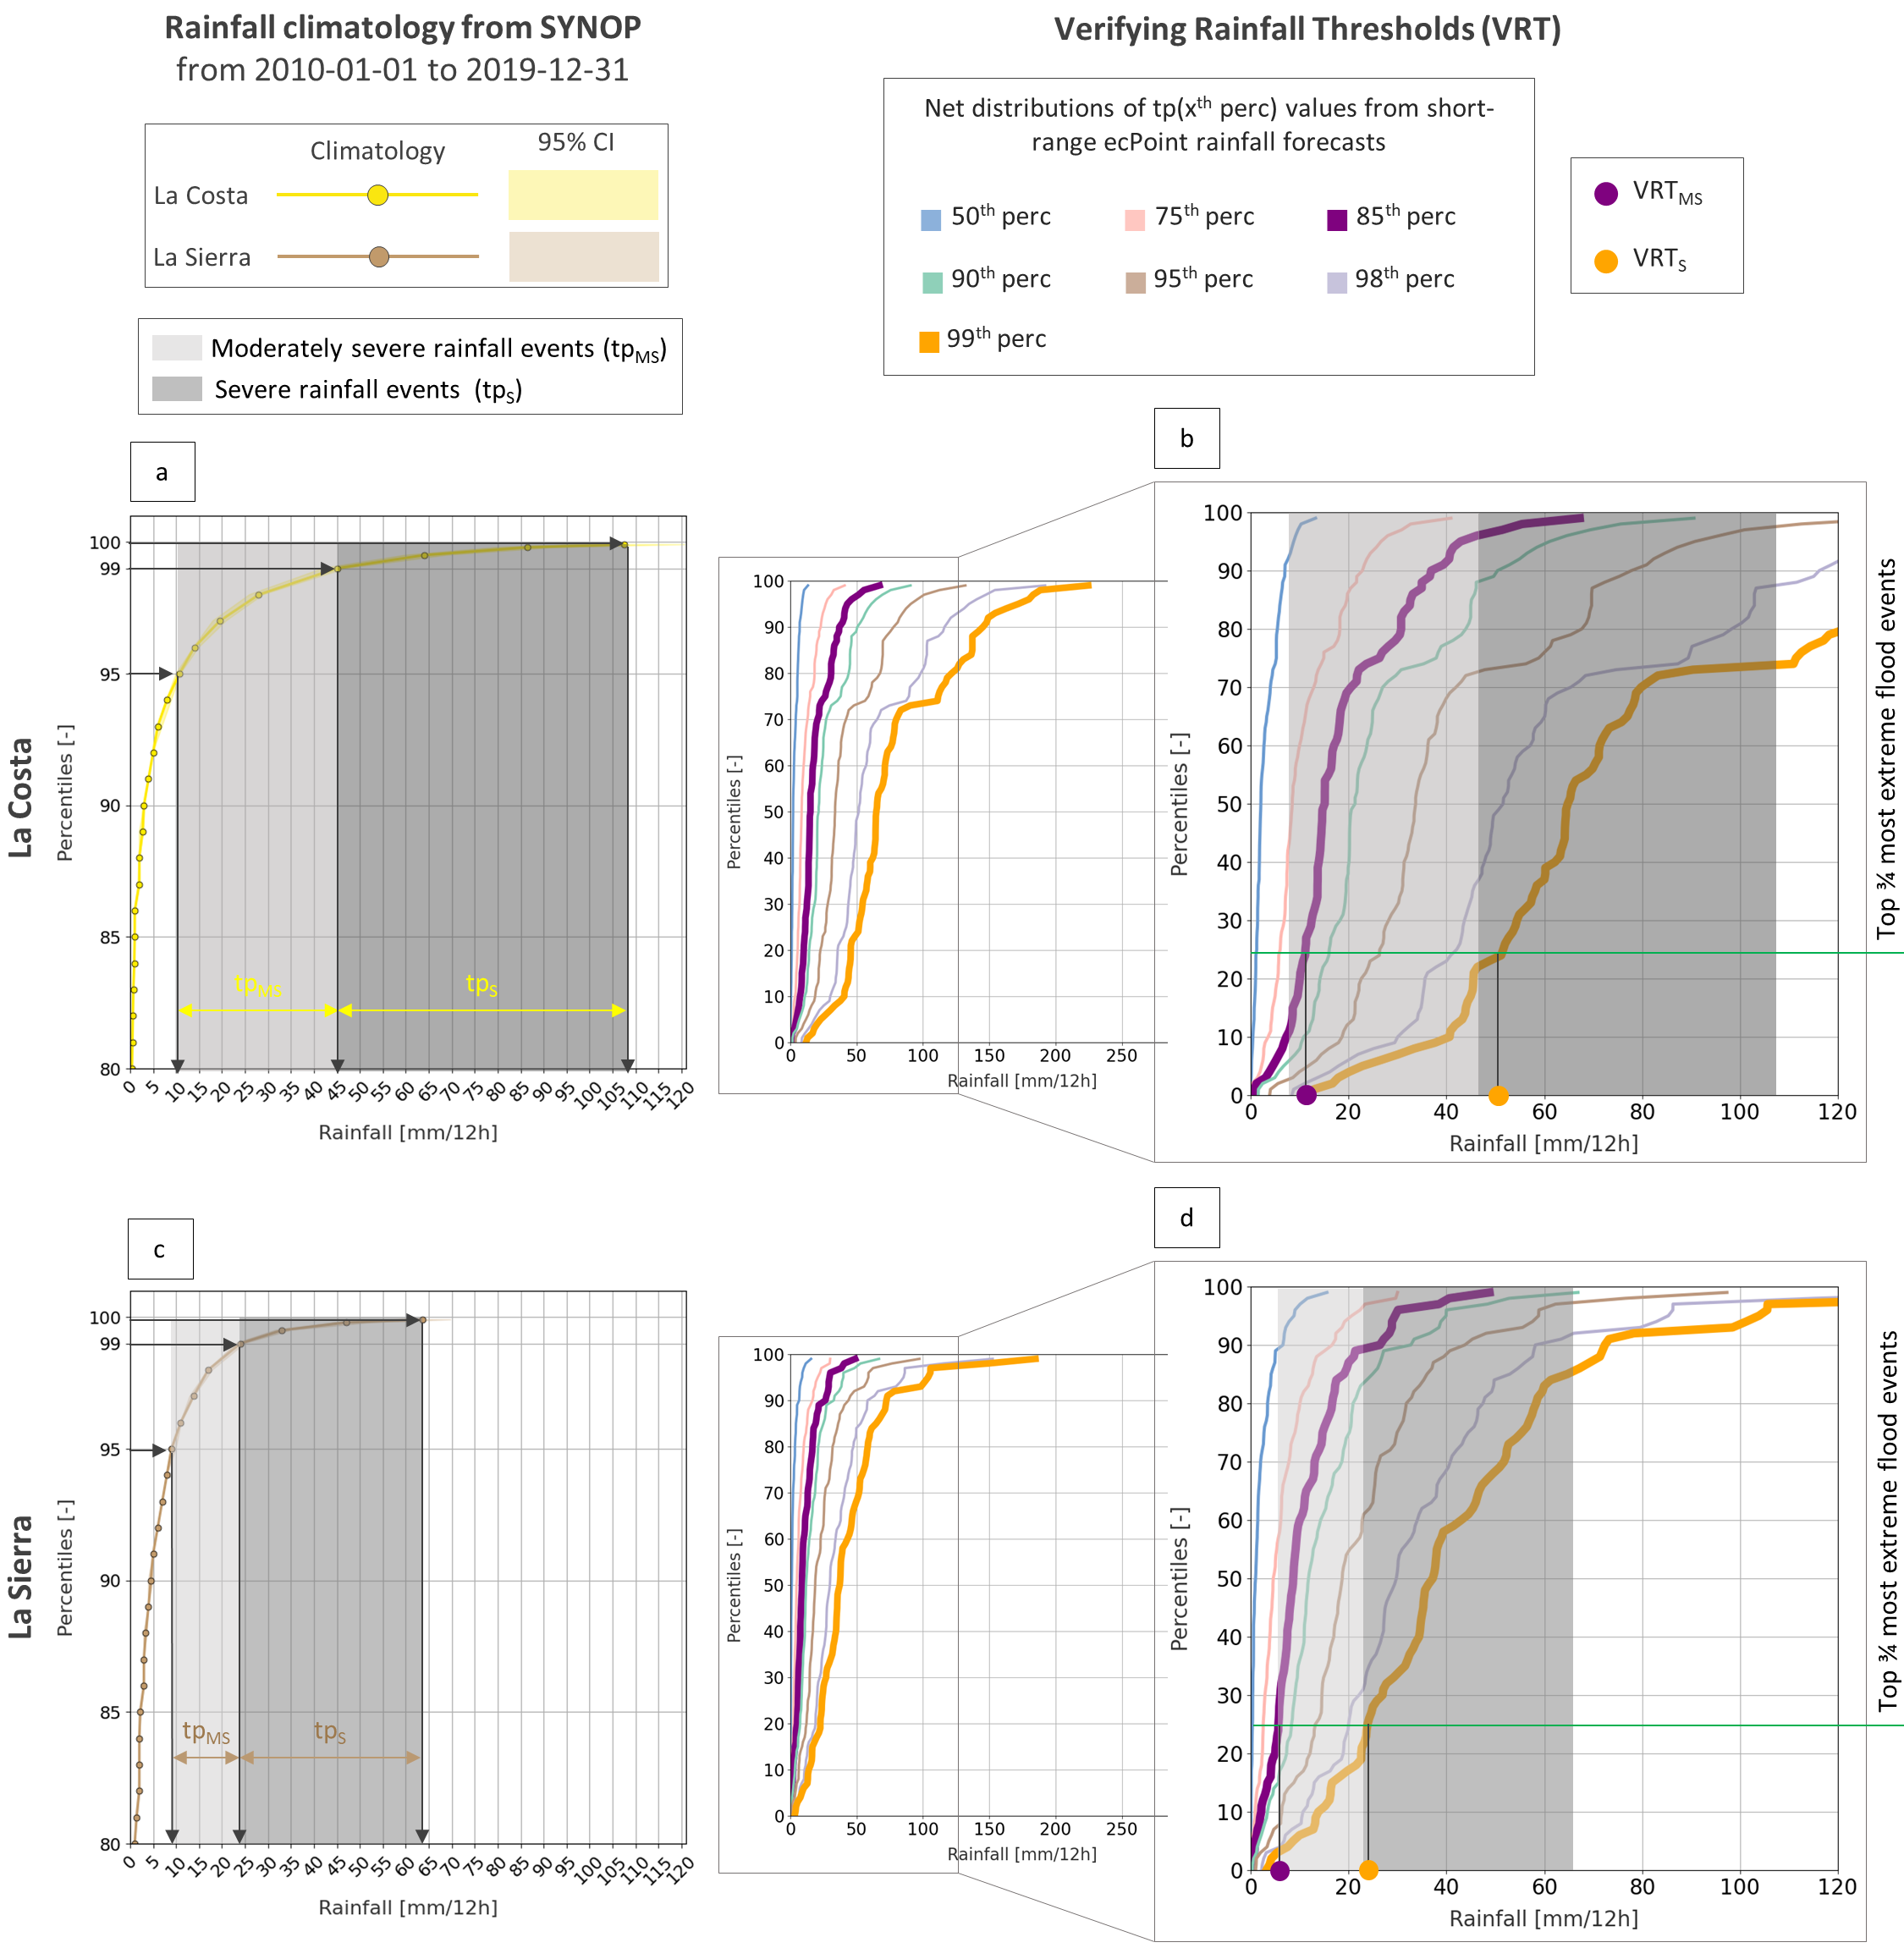
\includegraphics[width=\textwidth]{Figures/09_RESULTS_VRTs.png}
\caption{Panels (a) and (c) show the rainfall climatologies from SYNOP observations, respectively, for “La Costa” and “La Sierra”, with 95\% confidence intervals. The range of moderately severe (tp\textsubscript{MS}) and severe rainfall totals (tp\textsubscript{S}) are indicated, respectively, with a light and dark grey rectangle. Panels (b) and (d) show, respectively, the net distributions of flash-flood-triggering rainfall events (i.e., distribution in red in Figure \ref{fig:Methods_VRT}\hyperref[fig:Methods_VRT]{c}) for “La Costa” and “La Sierra”, built from the rainfall totals corresponding to the 50\textsuperscript{th} (in pale blue), 75\textsuperscript{th} (in pale pink), 85\textsuperscript{th} (in purple), 90\textsuperscript{th} (in pale green), 95\textsuperscript{th} (in pale brown), 98\textsuperscript{th} (in grey), and 99\textsuperscript{th} percentiles (in orange) in the distributions of short-range ecPoint rainfall forecasts (i.e., the xth percentile indicated in red in Figure \ref{fig:Methods_VRT}\hyperref[fig:Methods_VRT]{b}). The VRT\textsubscript{MS} (purple circle) and VRT\textsubscript{S} (orange circle) are defined using the net distribution that contains the cross point between the top 3/4 most extreme flood events and the lower threshold of, respectively, the range of moderately severe and severe rainfall events.}
\label{fig:Results_VRT}
\end{figure}

\begin{figure}
\centering
\captionof{table}{Verifying rainfall thresholds (in mm/12h).}
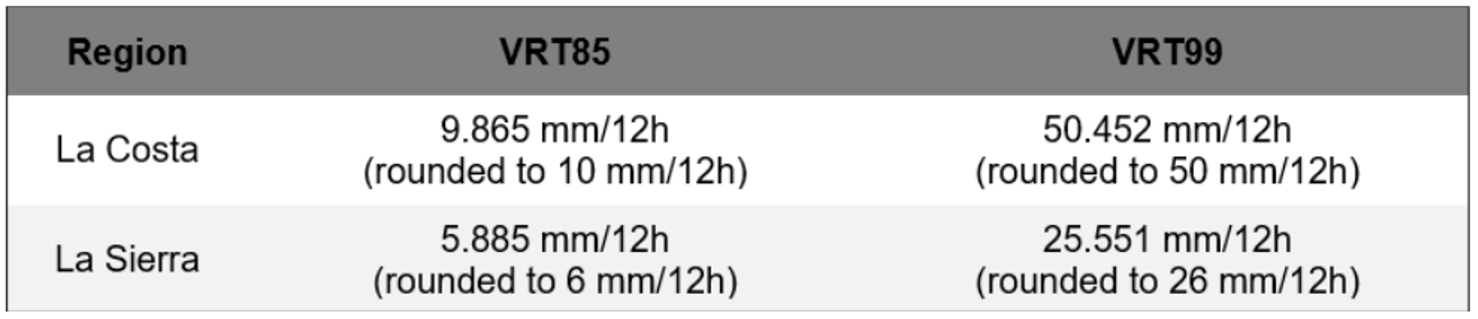
\includegraphics[width=0.5\textwidth]{Tables/04_VRTs.png}
\label{table:VRTs}
\end{figure}

The rainfall climatologies computed from the SYNOP observations show in “La Costa” (Figure \ref{fig:Results_VRT}\hyperref[fig:Results_VRT]{a}) ranges for tp\textsubscript{MS} (between 10 and 45 mm/12h) and tp\textsubscript{S} (between 45 and 108 mm/12h) that are much bigger than in “La Sierra” (Figure \ref{fig:Results_VRT}\hyperref[fig:Results_VRT]{c}), where tp\textsubscript{MS} ranges between 10 and 25 mm/12h and tp\textsubscript{S} ranges between 25 and 64 mm/12h. Considering these ranges, the net distributions of flash-flood-triggering rainfall events corresponding to the 50\textsuperscript{th} and 75\textsuperscript{th} percentiles provide rainfall values that are deemed too small (Figure \ref{fig:Results_VRT}\hyperref[fig:Results_VRT]{b} and Figure \ref{fig:Results_VRT}\hyperref[fig:Results_VRT]{d}). In both regions, the net distributions for the 85\textsuperscript{th}, 90\textsuperscript{th}, 95\textsuperscript{th}, and 98\textsuperscript{th} percentiles provide good candidates to define the VRT\textsubscript{MS}, while the net distribution for the 90\textsuperscript{th}, 95\textsuperscript{th}, and 98\textsuperscript{th}, and 99\textsuperscript{th} percentiles provide good candidates to define the VRT\textsubscript{S}. To increase the count of predicted moderately severe and severe events (and so produce robust statistics), it was decided to define the VRT\textsubscript{MS} and VRT\textsubscript{S} from the first net distribution (within the ranges provided) intersected by the horizontal line corresponding to retain the top 3/4 of the observed flood reports. Therefore, VRT\textsubscript{MS} and VRT\textsubscript{S} are defined from the net distribution corresponding to the 85\textsuperscript{th} and 99\textsuperscript{th} percentile. The VRT\textsubscript{MS} and VRT\textsubscript{S} are indicated by purple and orange dots in Figure \ref{fig:Results_VRT}\hyperref[fig:Results_VRT]{c} for “La Costa” and in Figure \ref{fig:Results_VRT}\hyperref[fig:Results_VRT]{f} for “La Sierra.” The rounded values in mm/12h, used in the objective verification analysis are listed in Table \ref{table:VRTs}.

\subsection{Objective verification}
\label{sec:Obj_Verif}

\subsubsection{Forecast discrimination ability}

\begin{figure}
\centering
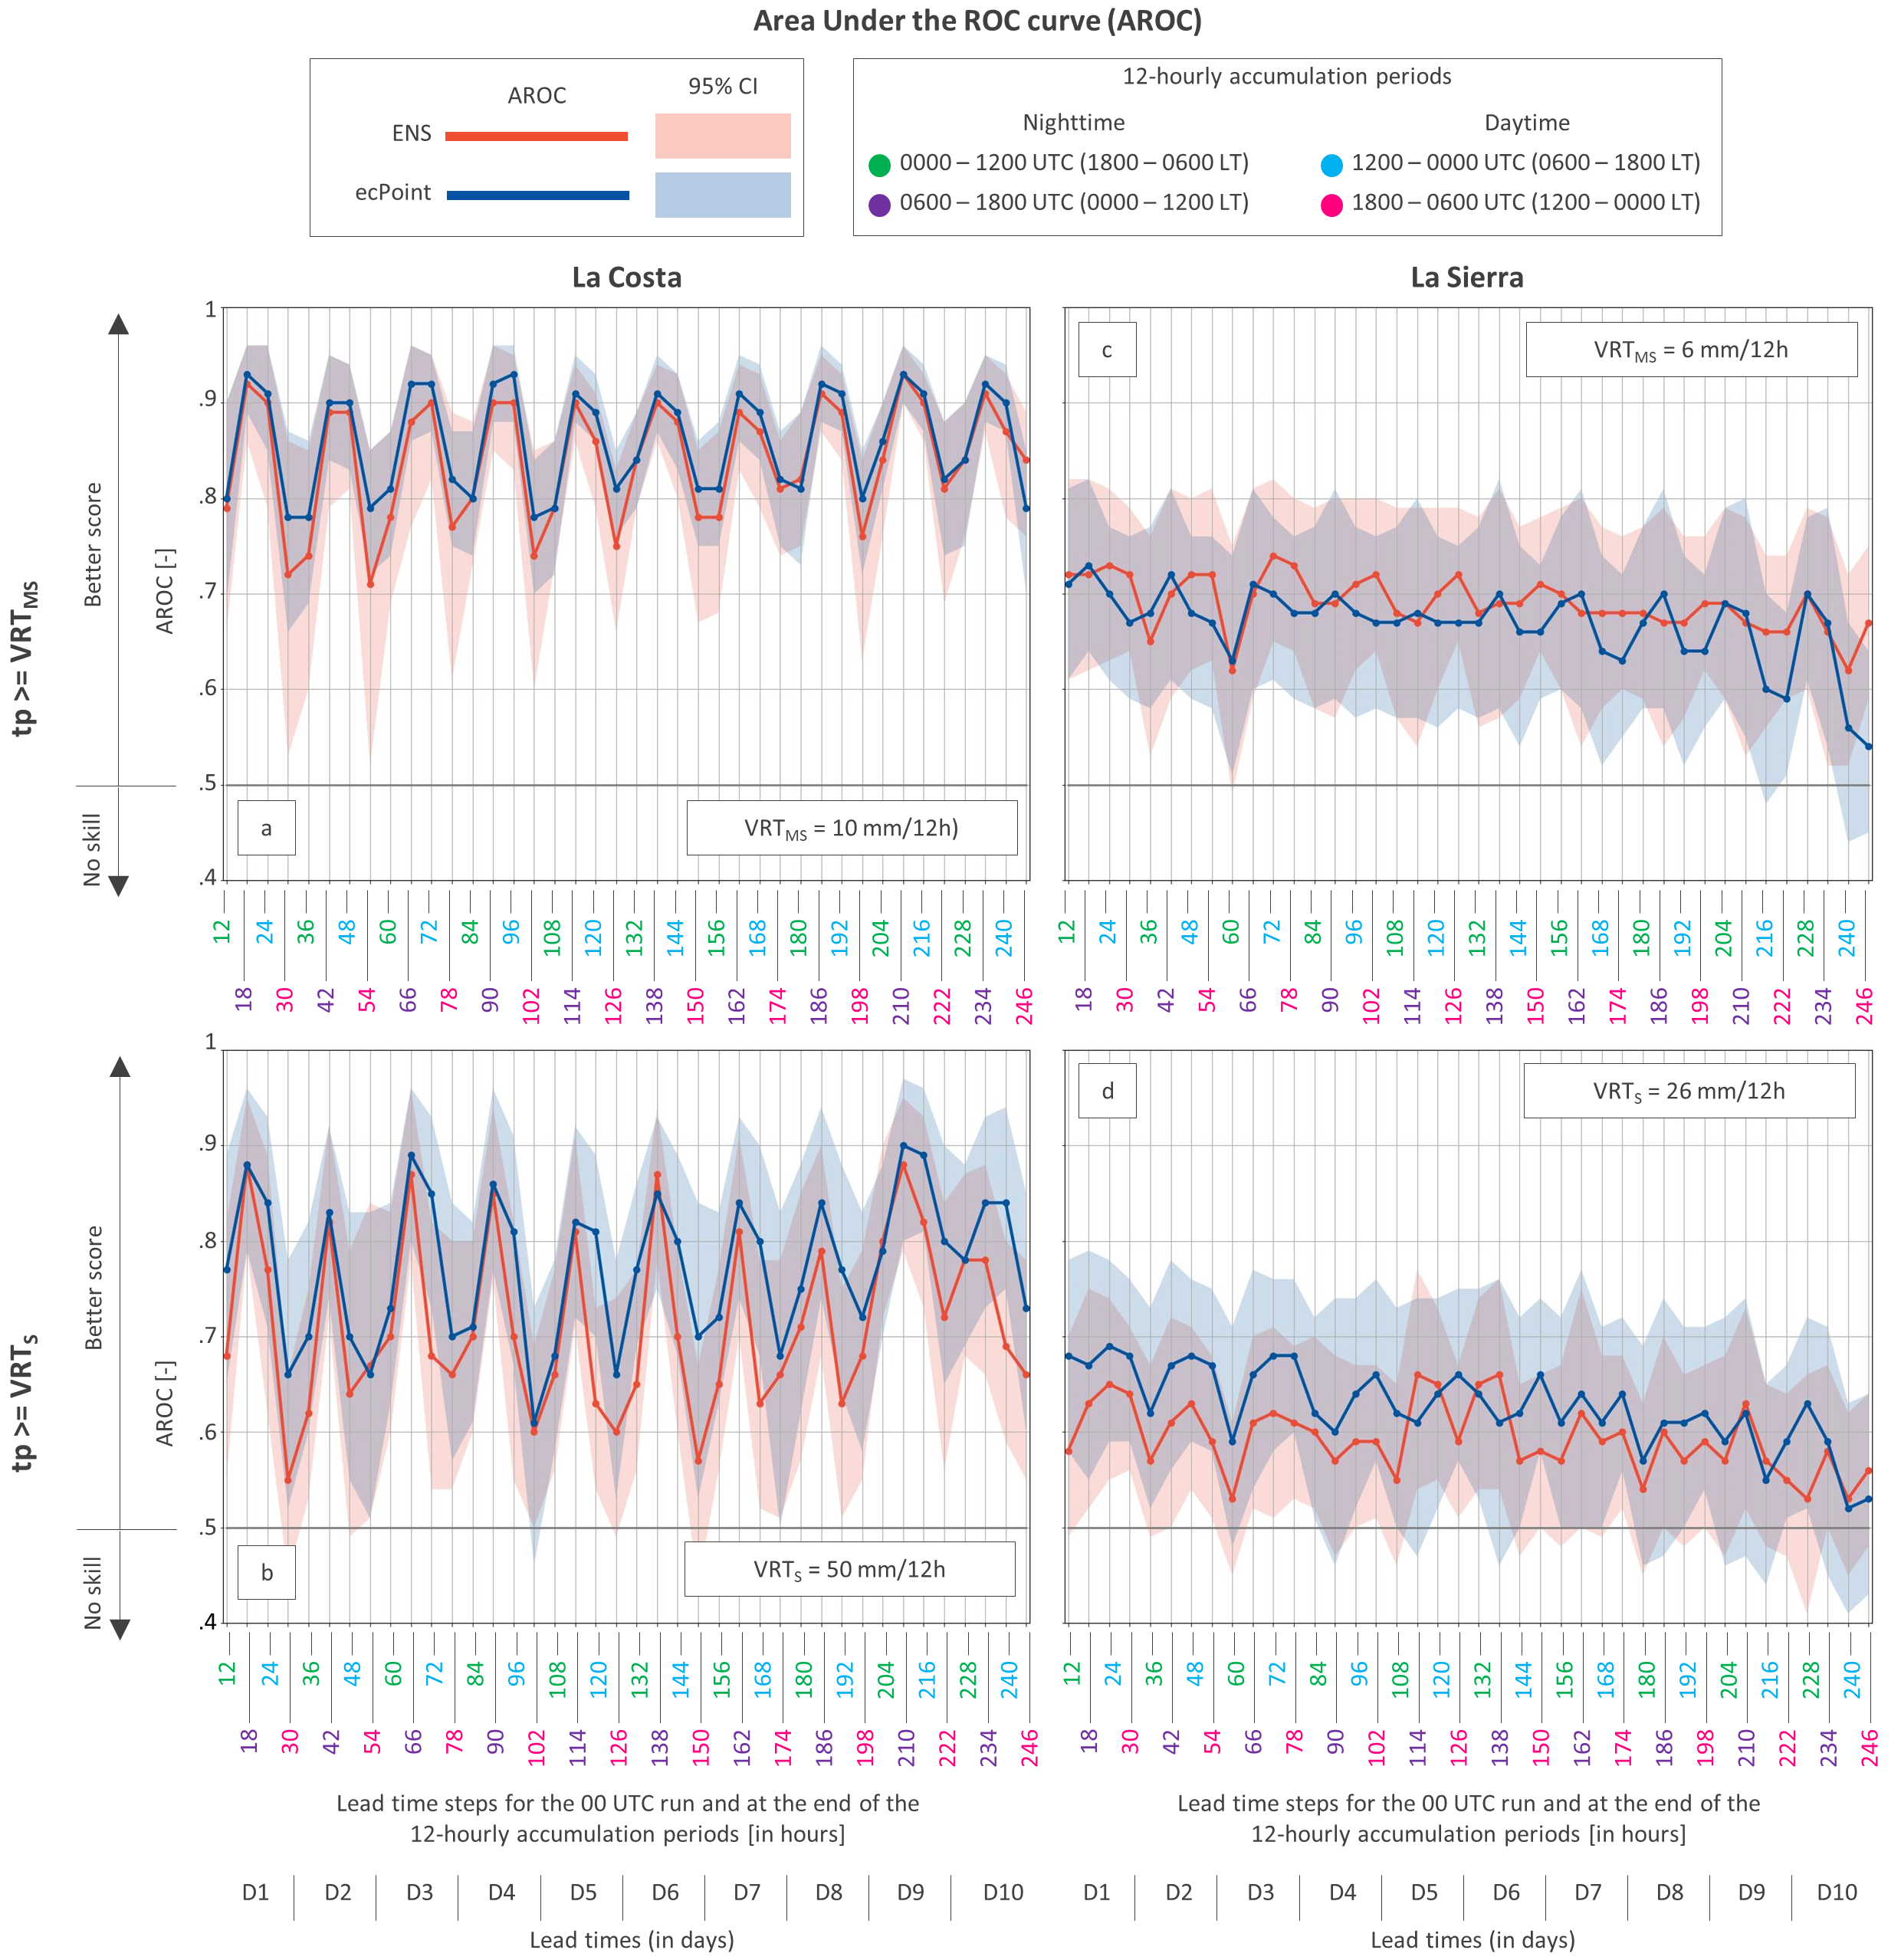
\includegraphics[width=\textwidth]{Figures/10_RESULTS_AROC.png}
\caption{Area under the ROC curve (AROC) for flood reports with EFFCI$\geq$6. Panels (a) and (b) show the AROC, respectively, for VRT\textsubscript{MS}$\geq$10 mm/12h and VRT\textsubscript{S}$\geq$50 mm/12h in “La Costa”. Panels (c) and (d) show the AROC, respectively, for VRT\textsubscript{MS}$\geq$6 mm/12h and VRT\textbf{S}$\geq$26 mm/12h in “La Sierra”. The lines and the shaded areas represent, respectively, the values of the AROC and the confidence interval (CI) at 95\% for ENS (in red) and ecPoint (in blue). The x-axis indicates the lead times steps for the 00 UTC run at the end of the 12-hourly accumulation period, expressed in hours. The colours associated with each step indicate the valid 12-hourly accumulation periods in UTC and local time (LT). The steps in green for 0000-1200 UTC (or 1800-0600 LT) and in purple for 0600-1800 UTC (or 0000-1200 LT) represent the 12-hourly accumulation periods during the night-time. The steps in cyan for 1200-0000 UTC (or 0600-1800 LT) and in fuchsia for 1800-0600 UTC (or 1200-0000 LT) represent the 12-hourly accumulation periods during the daytime. Lead times are also expressed in days (from 1 to 10).}
\label{fig:AROC}
\end{figure}

\begin{figure}
\centering
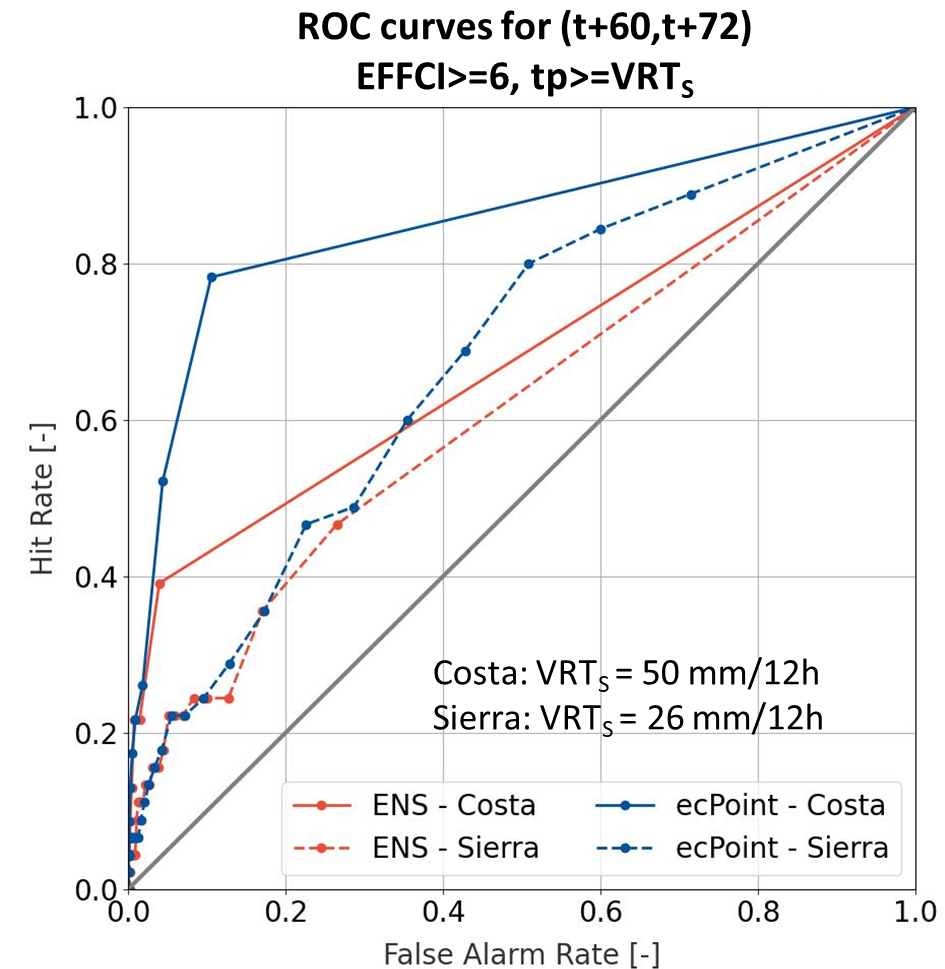
\includegraphics[width=0.5\textwidth]{Figures/11_RESULTS_ROCs.png}
\caption{ROC curves built with flood reports with EFFCI$\geq$6, for tp$\geq$VRT\textsubscript{S} and for the accumulation period between (t+60, t+72), i.e., for 0600 to 1800 local time (LT). The red and the blue lines denote, respectively, the ROC curves for ENS and ecPoint. The continuous and the dashed lines correspond to the ROC curves for “La Costa” and “La Sierra”.}
\label{fig:ROC}
\end{figure}

Figure \ref{fig:AROC}\ shows the evolution of the AROC with the lead time for VRT\textsubscript{MS} and VRT\textsubscript{S} for “La Costa” and “La Sierra.” No degradation of the AROC values with lead time was observed in “La Costa” (Figure \ref{fig:AROC}\hyperref[fig:AROC]{a} and Figure \ref{fig:AROC}\hyperref[fig:AROC]{b}), while there is some degradation observed in “La Sierra” (Figure \ref{fig:AROC}\hyperref[fig:AROC]{c} and Figure \ref{fig:AROC}\hyperref[fig:AROC]{d}). The AROC values for ENS and ecPoint diminished at the same rate for both VRT. Overall, the AROC values were larger for VRT\textsubscript{MS} (Figure \ref{fig:AROC}\hyperref[fig:AROC]{a} and Figure \ref{fig:AROC}\hyperref[fig:AROC]{c}) than for VRT\textsubscript{S} (Figure \ref{fig:AROC}\hyperref[fig:AROC]{b} and Figure \ref{fig:AROC}\hyperref[fig:AROC]{d}), and for “La Costa” (\ref{fig:AROC}\hyperref[fig:AROC]{a} and Figure \ref{fig:AROC}\hyperref[fig:AROC]{b}) compared to “La Sierra” (\ref{fig:AROC}\hyperref[fig:AROC]{c} and Figure \ref{fig:AROC}\hyperref[fig:AROC]{d}). A feature that stands out in all panels in Figure \ref{fig:AROC}, but especially in “La Costa,” is the sinusoidal pattern shown by the AROC in correspondence with the different accumulation periods throughout the day. In “La Costa” (Figure \ref{fig:AROC}\hyperref[fig:AROC]{a} and Figure \ref{fig:AROC}\hyperref[fig:AROC]{c}), the peaks in the AROC are observed between 0000-1200 LT (i.e., lead time steps labelled in purple) and 0600-1800 LT (i.e., lead time steps labelled in cyan, that correspond to rainfall occurred mainly during daytime), while troughs are mostly observed between 1200-0000 LT (i.e., lead time steps labelled in pink) and 1800-0600 LT (i.e., lead time steps labelled in green, that correspond to rainfall occurred mainly during night-time). Overall, the discrimination ability for ecPoint in “La Costa” tended to be better than the discrimination ability for ENS, especially for VRT\textsubscript{S} (Figure \ref{fig:AROC}\hyperref[fig:AROC]{c}). However, it is worth noting that ecPoint and ENS’s AROC values are closer in the peaks and further apart in the troughs, meaning that the improvements that ecPoint brings in the identification of areas at risk of flash floods are mainly over rainfall events occurring in the daytime. A similar sinusoidal pattern, although noisier, was observed for the AROC values in “La Sierra” (Figure \ref{fig:AROC}\hyperref[fig:AROC]{c} and Figure \ref{fig:AROC}\hyperref[fig:AROC]{d}). Unlike in “La Costa”, in “La Sierra” there are no specific times of the day where ecPoint adds value to the performance of ENS. For VRT\textsubscript{MS} (Figure \ref{fig:AROC}\hyperref[fig:AROC]{c}), ENS shows an overall better discrimination ability than ecPoint, while the latter shows an overall better performance than ENS in the AROC values for VRT\textsubscript{S} (Figure \ref{fig:AROC}\hyperref[fig:AROC]{d}).

The analysis of the ROC curves provides further information on the discrimination ability of forecasts. Figure \ref{fig:ROC} shows the ROC curves for ENS (in red) and ecPoint (in blue) for the 12-hourly accumulation period ending at t+72 (i.e., day 3 forecast), which corresponds to a mainly daytime rainfall whose valid accumulation period ends at 1800 LT. For both regions, the AROC is larger. However, substantial differences were observed in the shapes of ROC curves. For “La Costa” (continuous line), the ROC curves are mostly overlapping, and only the points corresponding to the two top percentiles in ecPoint (98\textsuperscript{th} and 99\textsuperscript{th}) are above the ROC curve for ENS. This means that the underlying curve for ENS and ecPoint is the same, and the greater AROC from ecPoint is due to the capability to identify extremes better thanks to the bigger number of ensemble members. In this case, it can be concluded that ENS contains the information required to predict whether an extreme flash-flood-triggering rainfall event might occur, although it might not be possible to predict the actual magnitude of the event. To achieve this goal, forecasts from ecPoint are better suited because they can double the hit rate from the ENS with only a very small increase in the false alarm rate. On the contrary, although noisy, it can be observed that the ROC curves in “La Sierra” (dashed lines) do not overlap. This implies that the underlying curves for ENS and ecPoint are different. Thus, ecPoint can identify events for which ENS may not provide any signal.  

\subsubsection{Forecast frequency bias}

\begin{figure}
\centering
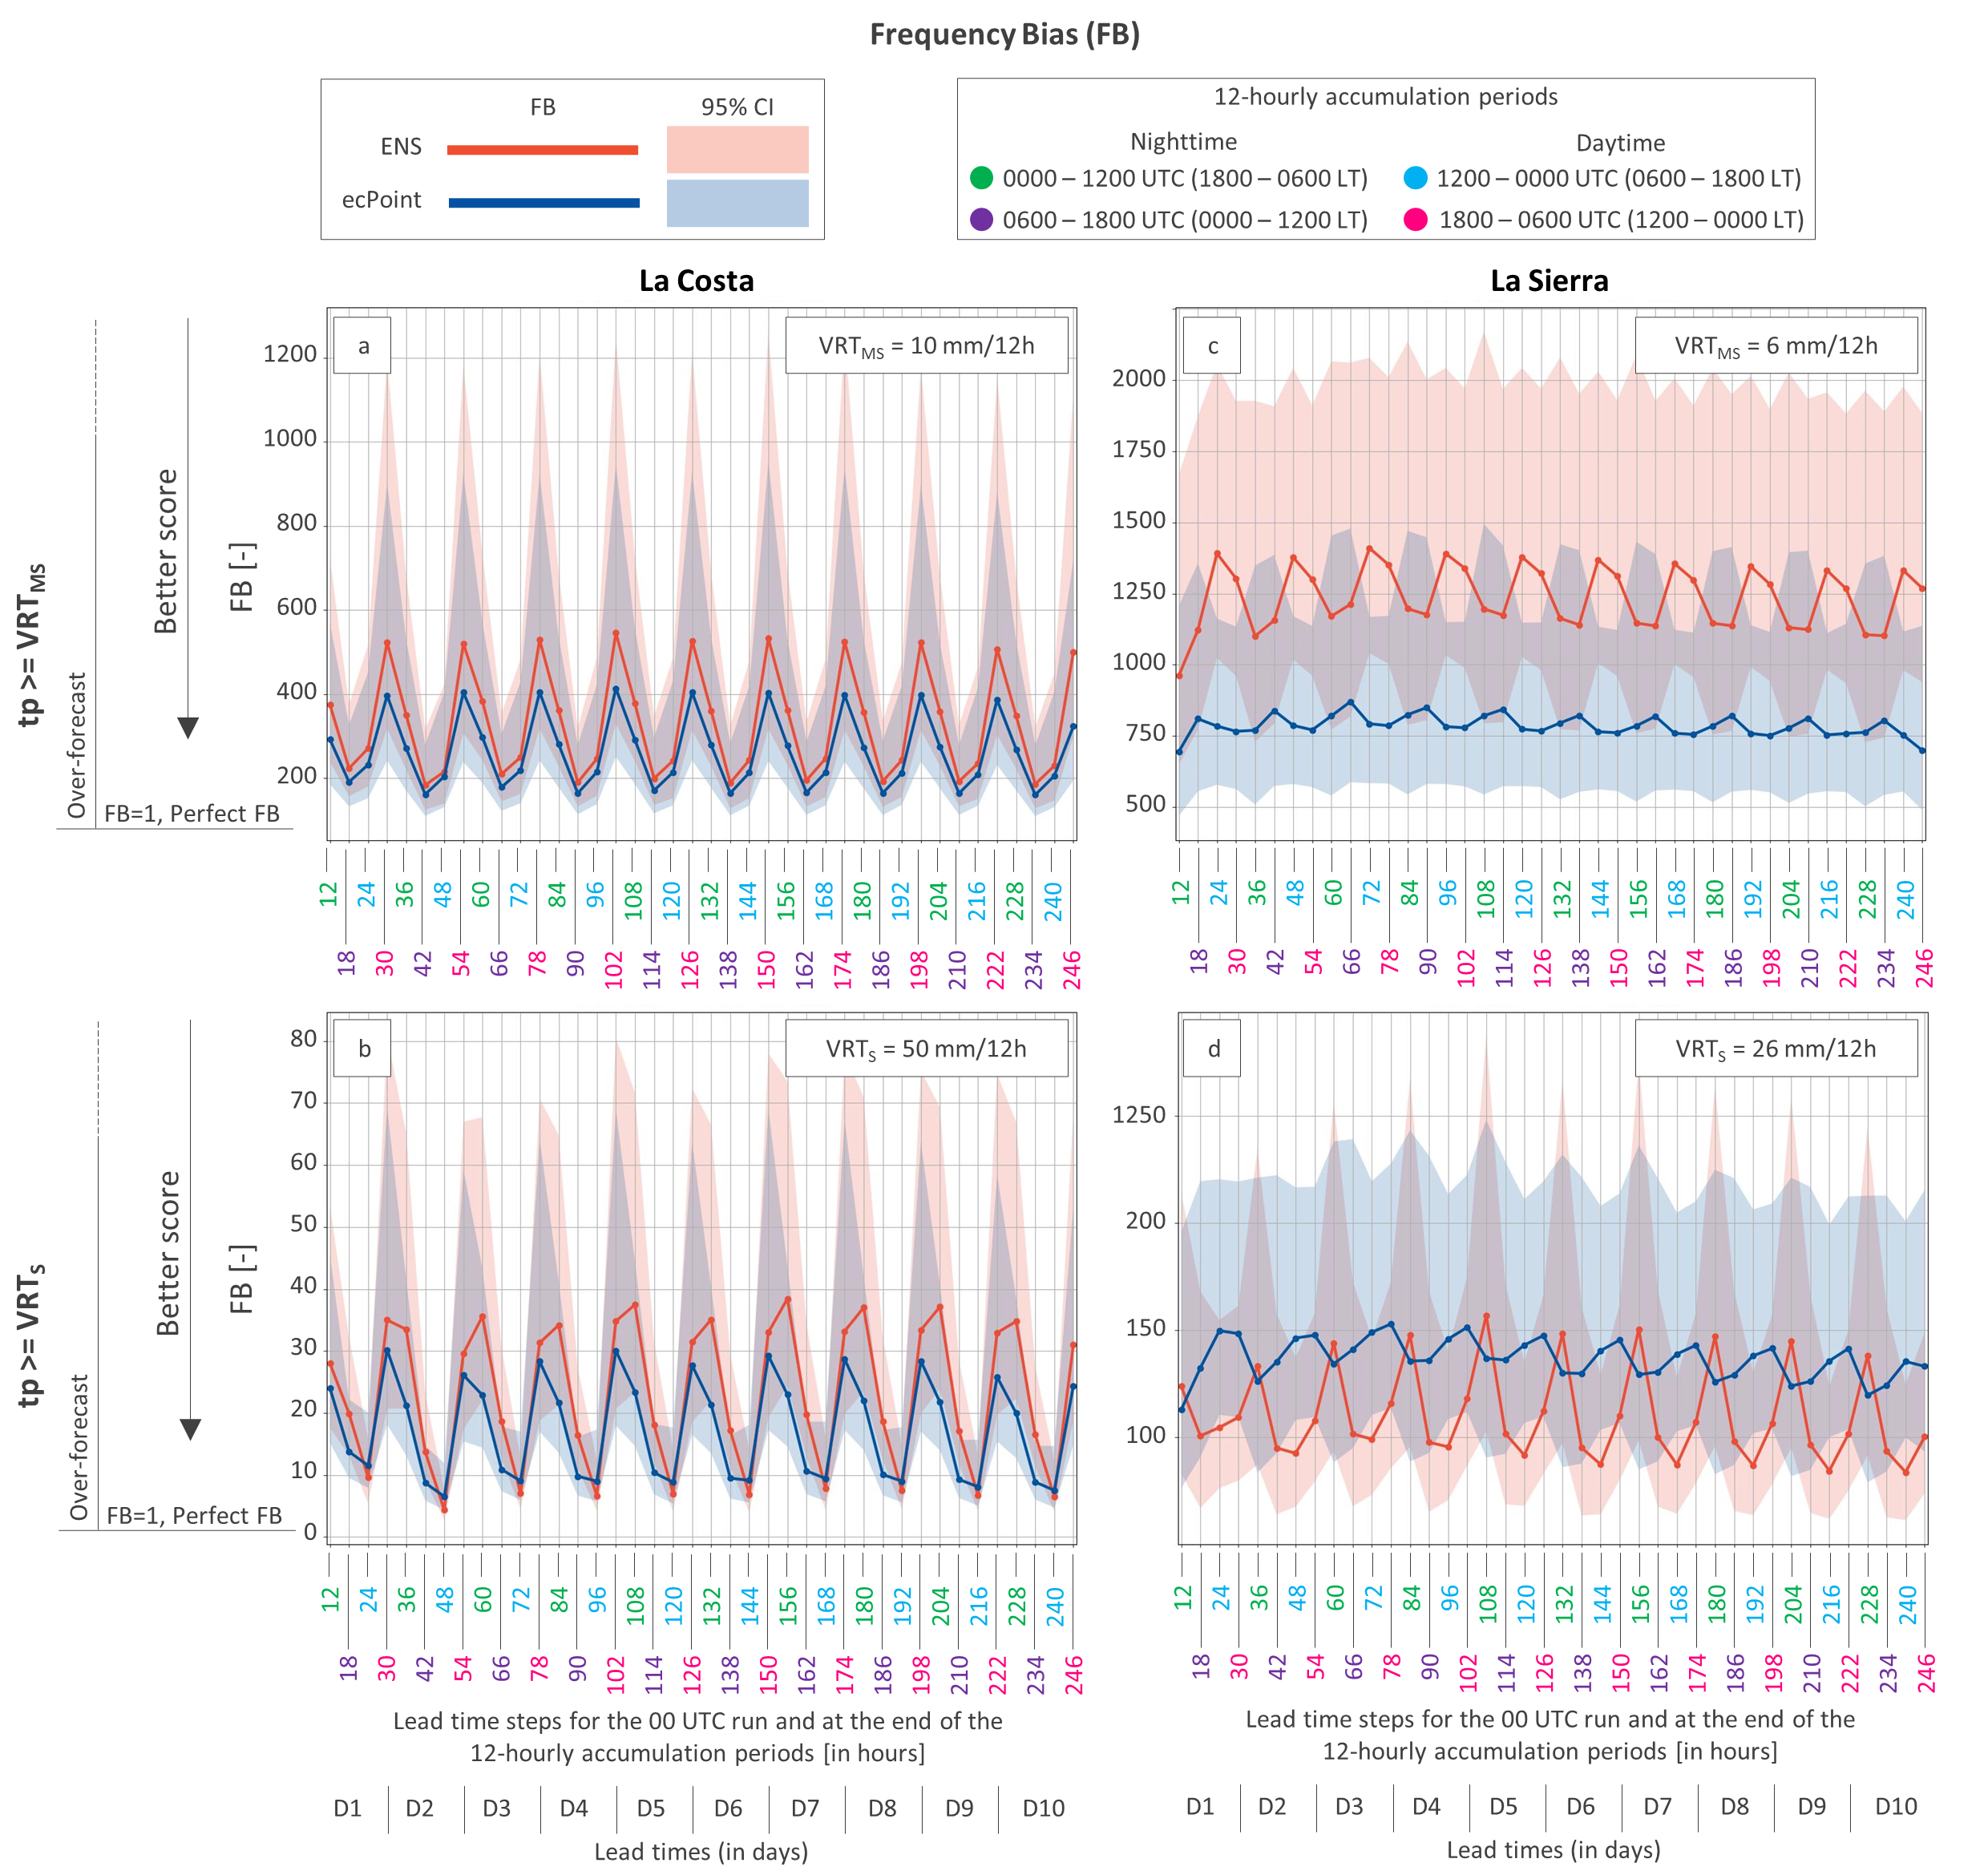
\includegraphics[width=\textwidth]{Figures/12_RESULTS_FB.png}
\caption{Frequency bias (FB) for flood reports with EFFCI$\geq$6. Panels (a) and (b) show the FB, respectively, for VRT\textsubscript{MS}$\geq$10 mm/12h and VRT\textsubscript{S}$\geq$50 mm/12h in “La Costa”. Panels (c) and (d) show the FB, respectively, for VRT\textsubscript{MS}$\geq$6 mm/12h and VRT\textsubscript{S}$\geq$26 mm/12h in “La Sierra”. The lines and the shaded areas represent, respectively, the values of the FB and the confidence interval (CI) at 95\% for ENS (in red) and ecPoint (in blue). The x-axis indicates the lead times steps for the 00 UTC run at the end of the 12-hourly accumulation period, expressed in hours. The colours associated with each step indicate the valid 12-hourly accumulation periods in UTC and local time (LT). The steps in green for 0000-1200 UTC (or 1800-0600 LT) and in purple for 0600-1800 UTC (or 0000-1200 LT) represent the 12-hourly accumulation periods during the night-time. The steps in cyan for 1200-0000 UTC (or 0600-1800 LT), and in fuchsia for 1800-0600 UTC (or 1200-0000 LT) represent the 12-hourly accumulation periods during the daytime. The lead times are also expressed in days (from 1 to 10).}
\label{fig:FB}
\end{figure}

\begin{figure}
\centering
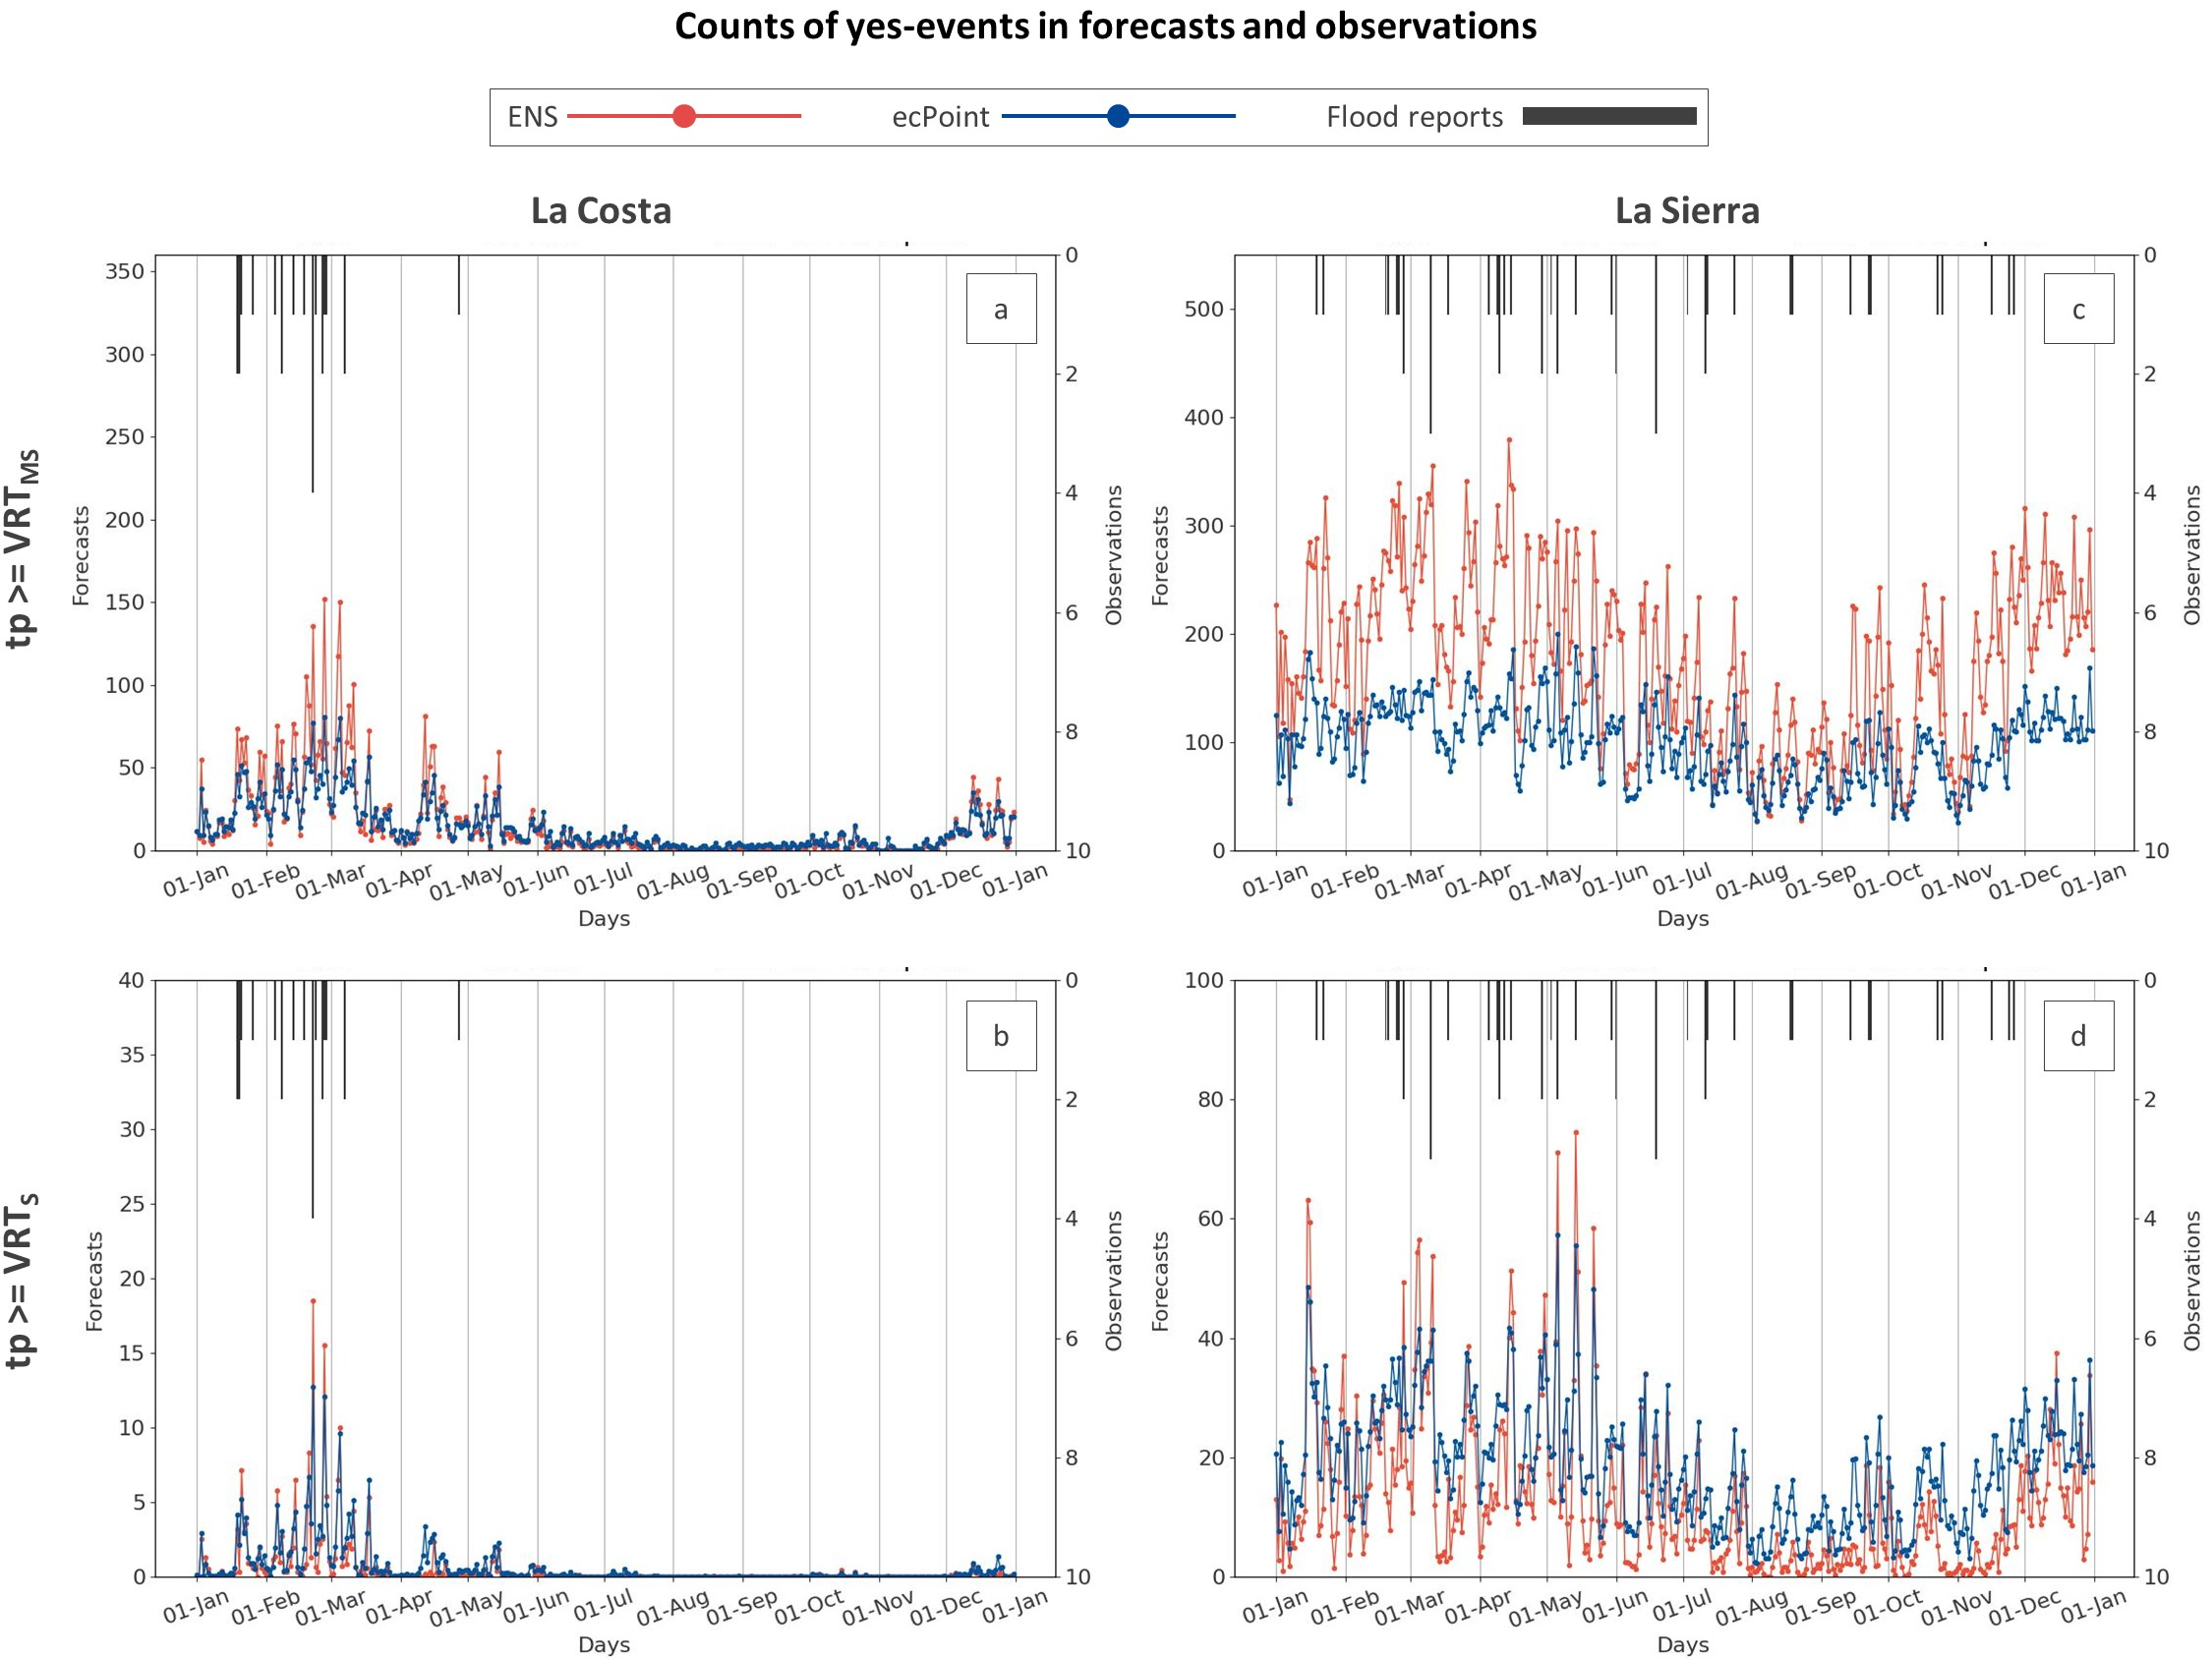
\includegraphics[width=0.8\textwidth]{Figures/13_RESULTS_Count_Yes_Events.jpg}
\caption{Counts of yes-events (flash floods) in forecasts and observations. The yes-events in the forecasts are displayed on the bottom x-axis, in red for ENS and in blue for ecPoint. The example considered is for the accumulation period ending at t+72 (day 3 forecast, daytime rainfall). The yes events in the observations are displayed in black on the top x-axis. Panels (a) and (b) show the counts for “La Costa” for tp$\geq$VRT\textsubscript{MS} and VRT\textsubscript{S}, respectively. Panels (c) and (d) show the same but for “La Sierra”.}
\label{fig:Counts_Yes_Events}
\end{figure}

Figure \ref{fig:FB} shows the evolution of the FB with lead time for VRT\textsubscript{MS} and VRT\textsubscript{S}, for “La Costa” and “La Sierra.” No significant degradation in FB was observed with the lead time in either region. Overall, FB is larger for VRT\textsubscript{MS} (Figure \ref{fig:FB}\hyperref[fig:FB]{a} and Figure \ref{fig:FB}\hyperref[fig:FB]{c}) than for VRT\textsubscript{S} (Figure \ref{fig:FB}\hyperref[fig:FB]{b} and Figure \ref{fig:FB}\hyperref[fig:FB]{d}), and for “La Sierra” (Figure \ref{fig:FB}\hyperref[fig:FB]{c} and Figure \ref{fig:FB}\hyperref[fig:FB]{d}) than for “La Costa” (Figure \ref{fig:FB}\hyperref[fig:FB]{a} and Figure \ref{fig:FB}\hyperref[fig:FB]{b}). In “La Costa,” ecPoint diminishes the FB at all lead times, but especially for the accumulation period that ends at 0000 LT (steps indicated in pink) in the case of VRT\textsubscript{MS} and for the accumulation period that corresponds to mainly night-time rainfall and ends at 0600 LT (steps indicated in green) in the case of VRT\textsubscript{S}. For the latter, only accumulation periods that correspond mainly to daytime rainfall and end at 1800 LT (steps indicated in cyan) show a slightly worse FB for ecPoint compared to ENS. ecPoint’s FB for VRT\textsubscript{MS} in “La Sierra” (Figure \ref{fig:FB}\hyperref[fig:FB]{c}) is significantly better than ENS’s FB, while for VRT\textsubscript{S} (Figure \ref{fig:FB}\hyperref[fig:FB]{d}) it is worse, with the exception of the accumulation periods that correspond mainly to night-time rainfall and end at 0600 LT (steps indicated in green). It is worth noting that opposite to what happens in “La Costa” where the performance is qualitatively the same for both forecasting systems (i.e., the peaks and troughs are observed for the same accumulation periods in both ENS and ecPoint), in “La Sierra” peaks and troughs happen in different accumulation periods for different forecasting systems. For VRT\textsubscript{MS}, peaks occurred for daytime rainfall in the ENS and for night-time rainfall in ecPoint. The opposite is true for the VRT\textsubscript{S}.

A feature that stands out in all panels in Figure \ref{fig:FB} is that the FB values are significantly larger than 1 (i.e., the perfect value for FB), indicating that ENS and ecPoint significantly overestimate the frequency of flash flood events. Figure \ref{fig:Counts_Yes_Events} shows the counts of yes-events in forecasts and observations for a day 3 forecast (i.e., accumulation period ending at t+72). In “La Costa” (Figure \ref{fig:Counts_Yes_Events}\hyperref[fig:Counts_Yes_Events]{a} and Figure \ref{fig:Counts_Yes_Events}\hyperref[fig:Counts_Yes_Events]{b}) there is a good overall correspondence between days with yes- and non-flash-flood events, especially for VRT\textsubscript{S}. The larger FB is mainly due to the slightly larger count of grid-boxes corresponding to yes events in the forecasts. In “La Sierra” (Figure \ref{fig:Counts_Yes_Events}\hyperref[fig:Counts_Yes_Events]{c} and Figure \ref{fig:Counts_Yes_Events}\hyperref[fig:Counts_Yes_Events]{d}), there is also a good representation of the periods with yes- and non-flash-flood events, especially for VRT\textsubscript{S}. However, the count of grid-boxes corresponding to yes-events in the forecasts is much larger than in the observations, contributing to FB values that are well above the perfect value of 1.   

%%%%%%%%%%%%%%%%%%%%%%%%%%%%%%%%%%%%%%%%%%%%%%%%%%%%%%%%%%%%%

\section{Case study: intense rainfall and flash floods on the 8\textsuperscript{th} of March 2021}
\label{sec:Case_Study}

This subjective verification analysis is presented to further support the outcomes of the objective verification analysis. March is one of the wettest months in 2021 in Ecuador. As a result of numerous heavy rainfall events, rivers such as Guayas, Los Ríos, Esmeraldas, and Manabí burst their banks, with landslides being observed in many different regions. The 8\textsuperscript{th} of March was one of the wettest days (Figure \ref{fig:Case_Study}). Significant impacts\footnote{https://www.eluniverso.com/guayaquil/comunidad/la-mayor-lluvia-del-2021-en-guayaquil-provoco-afectaciones-en-64-zonas-entre-inundaciones-arboles-caidos-canales-rebosados-y-otros-nota/} were mainly observed in the highly populated city of Guayaquil, where very heavy rainfall was reported to occur in the afternoon after 4 pm (Local Time, LT), with rainfall totals exceeding 100 mm/24h\footnote{https://www.wunderground.com/history/daily/SEGU/date/2021-3-8} in the city centre (zoomed red area in Figure \ref{fig:Case_Study}\hyperref[fig:Case_Study]{a}). Around the 8\textsuperscript{th} of March, the MJO was reported by various centres to be in phase 8\footnote{https://www.cpc.ncep.noaa.gov/products/precip/CWlink/MJO/ARCHIVE/PDF/mjo_evol-status-fcsts-20210315.pdf}, which tends to be conducive to, or at least correlated with, onshore lower tropospheric westerly wind anomalies near the equatorial west-facing coasts of South America \citep{Wheeler2004}. In conjunction, analysts from the NOAA have highlighted the likelihood of enhanced convective activity in the region in routine bulletins. ECMWF’s numerical model sounding (Figure \ref{fig:Case_Study}\hyperref[fig:Case_Study]{b}) valid for on the 8\textsuperscript{th} of March at 6 am (LT) appeared particularly conducive to flash-flood-triggering rainfall activity. For instance, the very high Convective Available Potential Energy (CAPE) shows that there is potential for sufficiently high dew point depression insolation-based triggering that might not be impeded by thick clouds. It also shows the potential for very high-altitude convective cloud tops, very strong wind shear that favours prolonged convective cell life cycles (as down-draughts would not interfere with up-draughts), and relatively light steering winds (favouring slow movement of convective cells). This description is supported by SYNOP and METAR observations and satellite imagery (not shown), suggesting that the cause of this rainfall event was organized convective cells, whose development was triggered by insolation. 

Figure \ref{fig:Case_Study}\hyperref[fig:Case_Study]{c} shows ENS and ecPoint rainfall forecasts from the 00 UTC run for day 1 (first row), day 3 (second row), and day 7 (third row) lead times. The forecasts are valid for the 12-hourly accumulation period between the 8\textsuperscript{th} of March 2021, at 12 am and the 9\textsuperscript{th} of March 2021, at 0 am (LT), that is, the fraction within the 24-hourly period of the observations reported in Figure \ref{fig:Case_Study}\hyperref[fig:Case_Study]{a} when most of the rainfall fell. Forecasts for the 50\textsuperscript{th} (first and second columns), 95\textsuperscript{th} (third and fourth columns), and 99\textsuperscript{th} percentiles (fifth and sixth columns) are shown. The median (i.e., 50\textsuperscript{th} percentile) represents the dividing line for the equi-probable observation categories. By comparing the rainfall observations (Figure \ref{fig:Case_Study}\hyperref[fig:Case_Study]{a}) and the forecast for the 50\textsuperscript{th} percentile (first and second columns in Figure \ref{fig:Case_Study}\hyperref[fig:Case_Study]{c}), it can be seen that, overall, the ENS overestimates the mean rainfall. On the contrary, owing primarily to its bias correction for rainfall overprediction at the grid-scale, ecPoint’s 50\textsuperscript{th} percentile is systematically smaller than in ENS, showing a better fit with the observations. At the same time, ecPoint’s 95th (third and fourth columns in Figure \ref{fig:Case_Study}\hyperref[fig:Case_Study]{c}) and 99\textsuperscript{th} percentiles (fifth and sixth columns in Figure \ref{fig:Case_Study}\hyperref[fig:Case_Study]{c}) highlight a higher potential than the ENS for having higher local rainfall totals in certain areas (e.g., Guayaquil). While far more observations would be needed to analyse robustly the performance of ENS and ecPoint forecasts for such a high percentile, it appears that both ENS and ecPoint predicted well the local rainfall extremes in “La Costa.” For example, there is a signal of extreme rainfall in the ENS for Guayaquil at the 95\textsuperscript{th} percentile). In contrast, it appears that ecPoint adds the most value to the prediction of extreme rainfall in “La Sierra.” For example, ecPoint’s 99\textsuperscript{th} percentile shows a 1\% chance of having up to 60 mm/12h at some location in “La Sierra”, and one location observed such an amount.

\begin{figure}
\centering
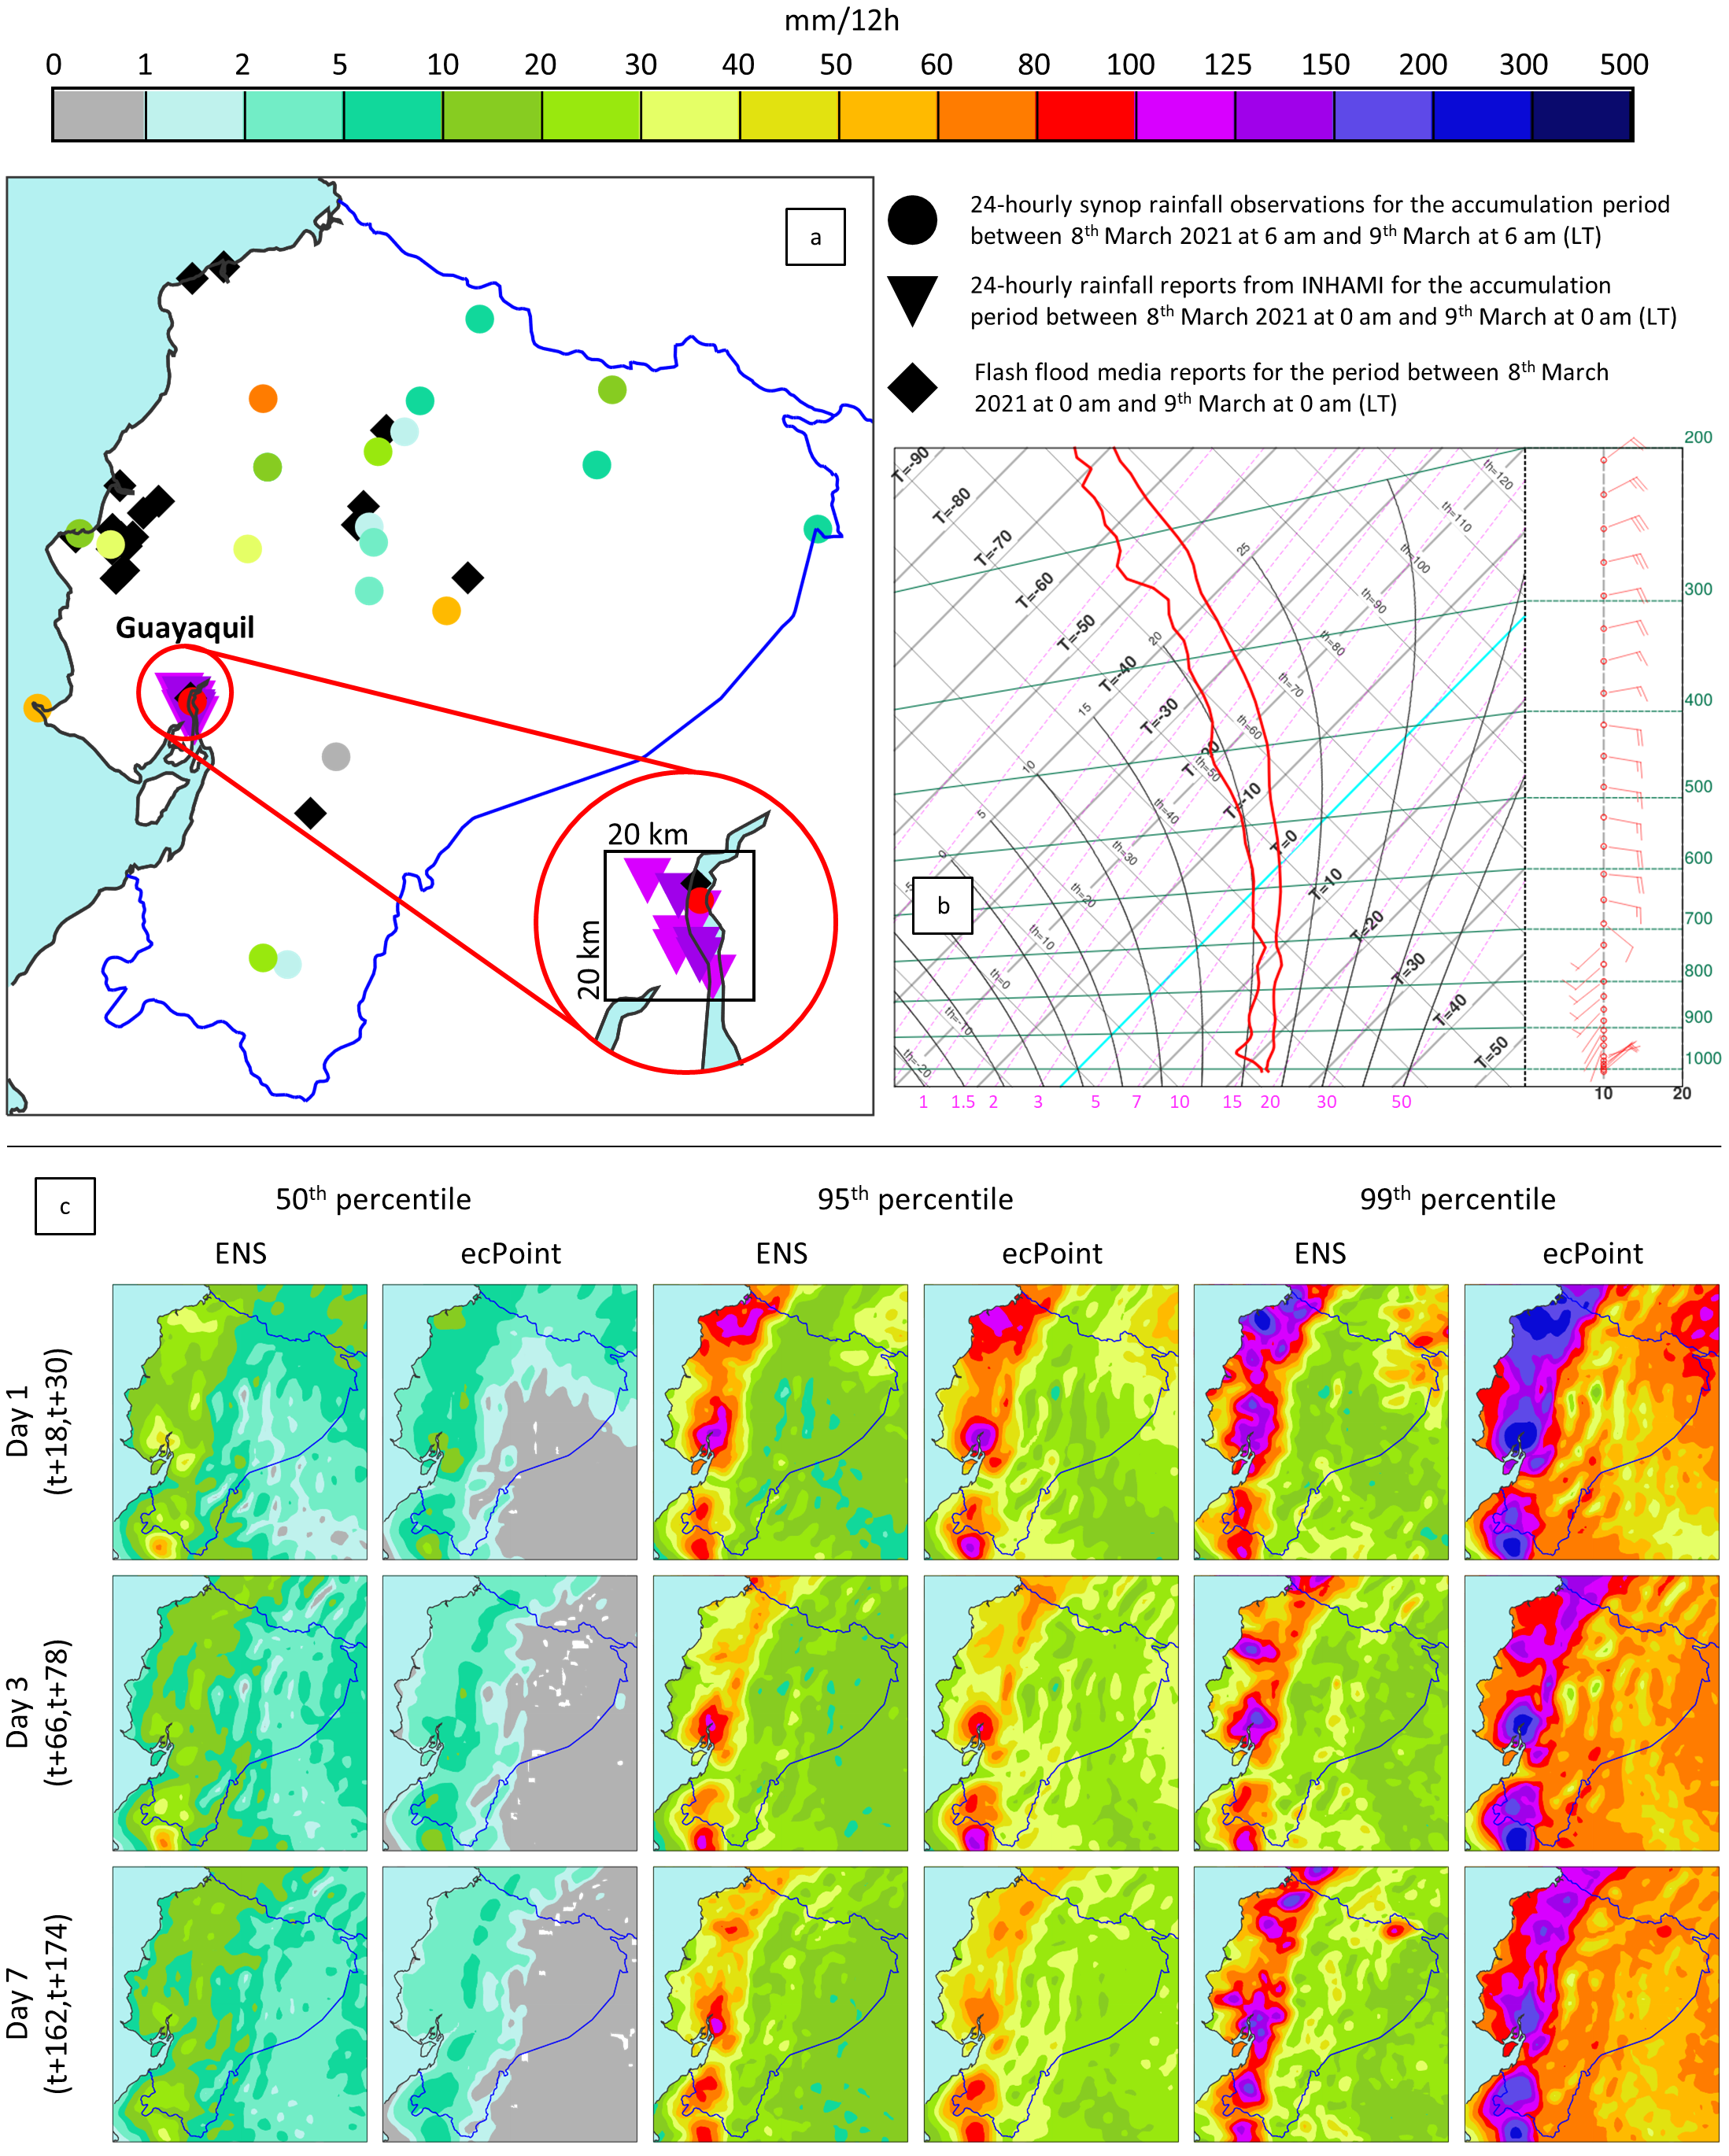
\includegraphics[width=0.9\textwidth]{Figures/14_CASESTUDY_Floods_March_2021.png}
\caption{Flash floods in Ecuador on 8\textsuperscript{th} March 2021. Panel (a) shows 24-hourly synop rainfall observations between 8\textsuperscript{th} March at 6 am and 9\textsuperscript{th} March at 6 am (coloured dots), 24-hourly rainfall reports from INAMHI for Guayaquil between 8\textsuperscript{th} March at 0 am and 9\textsuperscript{th} March at 0 am (coloured triangles), and flash flood reports in different regions between 8\textsuperscript{th} March at 0 am and 9\textsuperscript{th} March at 0 am (black diamonds). Panel (b) shows the sounding for Guayaquil (lat: -2.2; lon: -79.9) valid for 8\textsuperscript{th} March 2021 at 6 am. Panel (c) shows day 1, 3, and 7 forecasts from 00 UTC runs for ENS and ecPoint, valid for the accumulation period between 8\textsuperscript{th} March at 12 am and 9\textsuperscript{th} March at 0 am (when the rainfall event was at its peak). All reported times are meant to be in LT.}
\label{fig:Case_Study}
\end{figure}

%%%%%%%%%%%%%%%%%%%%%%%%%%%%%%%%%%%%%%%%%%%%%%%%%%%%%%%%%%%%%

\section{Discussion}
\label{sec:Discussion}

\subsection{Short-range ecPoint rainfall forecasts can be used as proxy for in-situ observations in data scares regions to calculate VRT}

The literature shows that the definition of flash-flood-triggering rainfall thresholds is a still widely used way to predict areas at risk of flash floods \citep{Ma2021, Papagiannaki2015, RamosFilho2021}. Central to these studies is the need for high-density rainfall observations to establish thresholds without excessive over- or underprediction biases. The lack of high-density, in situ 12-hourly rainfall observations in Ecuador would have limited the ability of defining the flash-flood-triggering rainfall thresholds, used in this study as VRT values. The method for calculating VRT values using ecPoint rainfall forecasts as a proxy for in-situ observations addresses this data gap by simulating a very high-density observational system in the proximity of the flash flood report. However, the probabilistic nature of the ecPoint output raises the following question: of all ecPoint’s rainfall realizations associated to a flash flood report, which amount represents better the one that triggered the corresponding flash flood event? The comparison of net distributions of potential flash-flood-triggering rainfall events with observational rainfall climatologies (even though computed using low-density point-rainfall observations) is essential to distinguish between net distributions that represent “moderately severe” rainfall events (i.e., events that might or might not generate flash floods), from net distributions that represent “severe” rainfall events, that are very likely to generate flash floods most of the times.

Several studies have found that flash flood forecasts are very sensitive to rainfall's spatial-temporal variability \citep{Borga2014, Demissie2021, Douinot2016, Norbiato2008, Song2019}. While the average rainfall does not seem to vary significantly in "La Sierra," the coastal areas in "La Costa" appear drier than on the western slopes of the Andes, suggesting that more than one VRT may be required to capture the variability in the magnitude of flash-flood-triggering rainfall events. Furthermore, the differences between daytime and night-time rainfall amounts suggest that a distinction between VRT values for daytime and night-time events could be beneficial to reduce biases in the verification analysis. Due to the limited availability of observational data, it was decided to aggregate all these conditions to provide more robust results, and only two VRT values were computed, one for the entire "La Costa" and one for the entire "La Sierra". However, this data aggregation comes at the expense of a greater granularity that might be beneficial and required to predict better areas at risk of flash floods. Finally, focusing solely on rainfall when defining VRT values may overlook other important factors. \cite{Dinis2021} highlighted how terrain and urban planning influence flash flood vulnerability in Benguela, Angola, even under moderate rainfall. Therefore, a more comprehensive approach incorporating geomorphological, socio-economic, and environmental factors alongside rainfall data is imperative for refining further the flash flood predictions and reducing false alarms.

\subsection{Comparison of ENS and ecPoint’s performance in the prediction of areas at risk of flash floods}

In Section \ref{sec:Background}, we learned that the meteorological dynamics influencing rainfall in “La Costa” and “La Sierra” are significantly different. This contextual backdrop is essential for interpreting the ENS and ecPoint performance in the identification of areas at flash flood risk in the two regions. In "La Costa", flash-flood-triggering rainfall events are generated predominantly by large-scale convective systems such as El Niño and the MJO \citep{Recalde-Coronel2020, Tobar2018}. ENS can predict with a reasonable degree of accuracy up to six weeks ahead of these systems \citep{Haiden2021}. Ergo, ENS can proficiently identify areas at risk of heavy rain (and flash floods), albeit it might still mis-forecast the absolute rainfall amounts. Herein, ecPoint’s contribution is primarily confined to rectifying the rainfall estimates. This type of correction is influential in continuous rainfall amount verification, but it becomes less relevant in binary event verification. Namely, it is not significant if a yes-event is obtained from exceeding the VRT by 1 mm or 20 mm as far as it is exceeded, and the correction of the absolute rainfall totals will matter only when it tips the balance between having or not having a yes-event. This behaviour can be observed for corrections applied by ecPoint to daytime and night-time rain in "La Costa". The needed reduction of daytime rain in “La Costa” applied by ecPoint to ENS forecasts is rewarded by both AROC and FB metrics. However, no significant changes in performance are observed when unnecessary corrections are applied to night-time rainfall (because the post-processing does not differentiate bias corrections depending on LT): ecPoint’s AROC values are the same as those for ENS, and the FB values are only slightly inferior. Conversely, flash-flood-triggering rainfall events in “La Sierra” are generated predominantly by small-scale convective systems \citep{Recalde-Coronel2014}. ENS struggles to capture extreme rainfall from such systems even on day 1, and when it does, its predictive skill decreases significantly after a few days \citep{Haiden2023}. \cite{Hewson2021} have shown that ecPoint significantly enhances the detection of small-scale convective systems and increases the lead time at which these systems can be identified in forecasts. As such, ecPoint has shown to perform better in identifying areas at risk of flash floods, especially for the most extreme flash flood events. The case-study-based analysis in Section \ref{sec:Case_Study} aligns with the discussion above. It indeed shows that ecPoint reduces the overprediction bias present in ENS while, at the same time, it improves ENS’s capability of predicting very extreme localised extreme rainfall events, especially when such an event is originated from a small-scale convective system.

These findings underscore the importance of considering the scale and nature of the weather systems that generate extreme rainfall in the region of interest when evaluating rainfall forecast performance in the identification of areas at risk of flash floods. When considering small-scale convective systems, ecPoint enhances structurally the performance of ENS, while whenever the main cause of extreme rainfall is a large-scale system, ENS can do a respectable job, and ecPoint would mainly help in predicting more accurately the entity (in mm) of the flash-flood-triggering rainfall events. This is consistent with the findings in \cite{Bucherie2022b}, who showed that larger-scale patterns linked to the occurrence of flash floods can be discerned in coarser global-scale models. This result is extremely important. So far, the research and the forecasting community have believed that km-scale rainfall forecasts were needed to identify areas at flash flood risk. However, this study establishes that raw global rainfall forecasts can be successfully used in the identification of areas at risk of flash floods under certain weather conditions. The two main benefits of being able to use global raw and post-processed NWP rainfall forecasts are (1) the availability of rainfall forecasts over a continuous domain (no more patchy coverage of km-scale limited-area models or radar-derived products) and (2) the availability of predictions up to medium-range lead times (instead of just a few hours or a couple of days). 

\subsection{Adequacy of the impact observations for verifying flash floods}

This study demonstrates that enhanced flood report databases, such as the one developed in Ecuador by \cite{Kruczkiewicz2021a}, are instrumental in setting flash-flood-triggering rainfall thresholds and assessing rainfall forecast performance in flash flood prediction. The better and more reliable spatial/temporal coverage of the flood reports in Ecuador’s database enabled an in-depth, long-term assessment that would have been unfeasible with publicly available flood reports due to their inevitably poorer spatial/temporal coverage and poorer identification of flood features (e.g., type of flood). For these reasons, flash flood verification in the past was primarily based on case studies as more detailed information was available for single events \citep{Gaume2009}. While a case-study-based verification approach is invaluable to understanding how forecasts predict flash flood events, provided enough observations are available, the results might not hold to other events due to the focused nature of the analysis. Alternatively, taking advantage of the better quality and spatial coverage of rainfall observations, researchers might use them to infer the performance of rainfall forecasts in predicting flash floods. However, as seen in this study, the results of these two verification analyses are different. ecPoint almost always performs better than ENS in predicting extreme (localized) rainfall \citep{Gascon2023, Hemri2022, Hewson2021}. However, in the binary prediction of  whether an area was affected by a flash food or not (yes- or no-event), the verification results are more nuanced. Not considering these two cases separately would do a disservice to the assessment of how well raw ENS forecasts can predict areas at risk of flash floods. Thus, this study underscores the importance of enhancing flash flood report databases to assess more in detail the performance of rainfall forecasts for flash flood prediction, contributing significantly to a more effective disaster preparedness and risk management strategies.

Although this dataset is the best attempt to build a comprehensive historical record of flash flood events in Ecuador, event underreporting still needs to be addressed to provide a more comprehensive assessment of forecast performance. In alignment with previous studies attempting to use impact-based observations to estimate forecast performance \citep{Hitchens2013, Mitheu2023, Robbins2018}, the verification of the rainfall forecasts against underreported flash flood events can lead to an underestimation of forecast skill and undermine the confidence in the forecasts, causing the dismissal of valuable predictions crucial for preparedness actions. It is, therefore, required to read beyond the actual numbers of verification results, and read them in a critical, although subjective, way. For example, although the FB is far larger than 1 (that would mean the forecasts overestimate substantially the areas at risk of flash floods), the counts of yes-events in the forecast and the observations show there is a good correspondence between wet/dry conditions (meaning the forecasts can identify fairly well which areas are at risk of flash floods) and that the high FB might be due mainly to the low spatial coverage of the reports. Techniques such as assigning 1s (i.e., yes-events) to adjacent grid-boxes to those already containing flood reports could help to reduce significantly the FB. We argue, however, that this method is more appropriate for forecasts provided on higher resolution grids because rainfall might not be predicted at the right location and/or the flash flood event might extend to adjacent grid-boxes. Since forecasts are here provided on a grid at 18 km, if a flash-flood-triggering rainfall event is predicted within a grid-box, it is reasonable to think that there is a good chance to see the flash flood within that grid-box (unless the event happens on the grid-box boundary, but this is an exception whose handling goes beyond the scope of this analysis). It  is, therefore, argue here that, when verifying global NWP forecasts, improvements in the observational spatial coverage are the way to reduce the number of “false” false alarms, which for this type of analysis (using non-standard observations) is the biggest and most difficult problem to address \citep{Marsigli2021}.

%%%%%%%%%%%%%%%%%%%%%%%%%%%%%%%%%%%%%%%%%%%%%%%%%%%%%%%%%%%%%

\section{Conclusions}
\label{sec:Conclusions}

This study defined a new method to calculate VRT values in data-scarce regions. By using short-range ecPoint rainfall forecasts as proxies for in-situ observations to calculate them, this method addresses significant data gaps that limit the verification and creation of flash flood forecasting systems in data-scarce regions. 

The performance of two global rainfall forecasts, ENS and ecPoint, is critically examined in identifying areas at risk of flash floods in Ecuador. It highlighted the nuances in the performance of the two forecasting systems in different meteorological contexts. While ecPoint outperforms ENS when flash-flood-triggering rainfall events are mainly originated from small-scale convective systems, in the case of large-scale systems ENS and ecPoint show comparable performance in the identification of areas at risk of flash floods, with ecPoint enhancing primarily only the accuracy of the magnitude prediction of the flash-flood-triggering rainfall event.

Finally, while the quality of the flash flood report database built for Ecuador is much higher than other public databases, this study has also discussed the impacts in objective flash flood forecast verification of a still large event underreporting. While the enhanced quality of the database used in this analysis allowed the authors to conduct an in-depth, long-term verification analysis, there is still work to do better assess forecast performance to support preparedness and action during decision-making processes.

The authors of this study suggest that future research should be focused in two main areas. Since the definition of flash-flood-triggering rainfall thresholds is linked to the availability of flash flood reports and those are not uniformly available around the globe, it would not be possible to develop rainfall-base flash flood forecasting systems over a continuous global domain. It would be interesting to develop an ecPoint-compatible gridded rainfall climatology, for example using the newly developed ERA5-ecPoint \citep{Hewson2023}, to create flash-flood-triggering rainfall thresholds over a continuous global domain and support the development of a rainfall-based flash flood forecasting system over the same domain. The authors also suggest that more resources are spent in the development of more flood databases like the one presented in this study as they incorporate invaluable details on the type of flood that can be used to target verification and forecast development efforts. At the same time, research efforts should be focused in addressing the uncertainties around the spatial coverage of this type of observations to provide clearer guidance on forecast performance.

%%%%%%%%%%%%%%%%%%%%%%%%%%%%%%%%%%%%%%%%%%%%%%%%%%%%%%%%%%%%%
\bibliographystyle{rss} \bibliography{ref}
\end{document}